%%%%%%%%%%%%%%%%%%%%%%%%%%% asme2ej.tex %%%%%%%%%%%%%%%%%%%%%%%%%%%%%%%
% Template for producing ASME-format journal articles using LaTeX    %
% Written by   Harry H. Cheng, Professor and Director                %
%              Integration Engineering Laboratory                    %
%              Department of Mechanical and Aeronautical Engineering %
%              University of California                              %
%              Davis, CA 95616                                       %
%              Tel: (530) 752-5020 (office)                          %
%                   (530) 752-1028 (lab)                             %
%              Fax: (530) 752-4158                                   %
%              Email: hhcheng@ucdavis.edu                            %
%              WWW:   http://iel.ucdavis.edu/people/cheng.html       %
%              May 7, 1994                                           %
% Modified: February 16, 2001 by Harry H. Cheng                      %
% Modified: January  01, 2003 by Geoffrey R. Shiflett                %
% Use at your own risk, send complaints to /dev/null                 %
%%%%%%%%%%%%%%%%%%%%%%%%%%%%%%%%%%%%%%%%%%%%%%%%%%%%%%%%%%%%%%%%%%%%%%

%%% use twocolumn and 10pt options with the asme2ej format
\documentclass[twocolumn,10pt]{asme2ej}

\usepackage{graphicx} %% for loading jpg figures
\usepackage{hyperref}   % to set up hyperlinks
\usepackage{amsmath}
\usepackage{csquotes}
\usepackage{enumitem}
\usepackage{float}
\usepackage{booktabs}
\allowdisplaybreaks
\hypersetup{
	colorlinks=true,
	linkcolor=blue,
	citecolor=blue,
	urlcolor=blue,
}

\usepackage[square,numbers]{natbib}

%% The class has several options
%  onecolumn/twocolumn - format for one or two columns per page
%  10pt/11pt/12pt - use 10, 11, or 12 point font
%  oneside/twoside - format for oneside/twosided printing
%  final/draft - format for final/draft copy
%  cleanfoot - take out copyright info in footer leave page number
%  cleanhead - take out the conference banner on the title page
%  titlepage/notitlepage - put in titlepage or leave out titlepage
%  
%% The default is oneside, onecolumn, 10pt, final


\title{Flow noise estimation models for axial flow past towed
sonar arrays}

%%% first author
\author{Rakesh Sekharipuram Sekar
    \affiliation{
	Student\\
	Department of Mechanical Engineering\\
	Indian Institute of Technology Palakkad\\
	Kanjikode, Palakkad, Kerala, 678623\\
	India\\
    Email: 132203001@smail.iitpkd.ac.in
    }	
}

%%% second author
%%% remove the following entry for single author papers
%%% add more entries for additional authors
\author{Senthil Rajan S
    \affiliation{ Scientist\\
	Naval Physical and Oceanographic Laboratory\\
	Kochi, Kerala, 682021\\
	India\\
        Email: senthilrajan.npol@gov.in
    }
}

%%% third author
%%% remove the following entry for single author papers
%%% add more entries for additional authors
\author{Dr. Anoop Akkoorath Mana\thanks{Address all correspondence related to ASME style format and figures to this author. Address all correspondence for other issues to this author.}
\affiliation{
        Assistant Professor\\
    Department of Mechanical Engineering\\
	Indian Institute of Technology Palakkad\\
	Kanjikode, Palakkad, Kerala, 678623\\
	India\\
    Email: akkoorath@iitpkd.ac.in
    }
}


\begin{document}

\maketitle    

%%%%%%%%%%%%%%%%%%%%%%%%%%%%%%%%%%%%%%%%%%%%%%%%%%%%%%%%%%%%%%%%%%%%%%
\begin{abstract}
{\it Towed sonar arrays house a series of pressure sensors inside a fluid-filled elastic tube. Towing of the sonar array in water generates a turbulent boundary layer on the exterior surface of the elastic tube. The pressure fluctuations in the turbulent boundary layer along with other ambient pressure fluctuations, excites the elastic tube and further generates pressure disturbances in the interior fluid. In this work, a new semi-empirical model of the turbulent pressure spectrum is presented. The new model predictions show a closer agreement with the available experimental results at all tow speeds. A three-dimensional vibroacoustic model of the fluid-filled elastic tube is also presented in this work. The vibroacoustic model is fully coupled and considers both breathing mode and first order variations in the elastic tube and the acoustic field variables. Further, the turbulent pressure spectrum semi-empirical model and the three-dimensional vibroacoustic model are used to compute the on-axis sound pressure level due to the external turbulent pressure excitation at different elastic tube diameters and tow speeds. At low frequencies, increasing tube diameter has little effect on flow noise, while at higher frequencies, flow noise decreases with larger diameters. Increasing tow speed raises flow noise across all frequencies.  
}
\end{abstract}

%%%%%%%%%%%%%%%%%%%%%%%%%%%%%%%%%%%%%%%%%%%%%%%%%%%%%%%%%%%%%%%%%%%%%%
\begin{nomenclature}
\entry{A}{You may include nomenclature here.}
\entry{$\alpha$}{There are two arguments for each entry of the nomemclature environment, the symbol and the definition.}
\end{nomenclature}

The primary text heading is  boldface and flushed left with the left margin.  The spacing between the  text and the heading is two line spaces.

%%%%%%%%%%%%%%%%%%%%%%%%%%%%%%%%%%%%%%%%%%%%%%%%%%%%%%%%%%%%%%%%%%%%%%
\section{Introduction}

Towed sonar arrays contain a series of pressure sensors enclosed within a fluid-filled elastic tube. As the sonar array is towed through the water, a thick layer of turbulent flow is generated over the exterior surface of the tube.~The pressure fluctuations in this turbulent boundary layer (TBL), along with other ambient sea pressure variations, excite the elastic tube and subsequently produce acoustic pressure disturbances within the interior fluid. The hydrophones placed in the interior fluid picks these acoustic signals. The signals associated with the turbulent pressure fluctuations are called flow noise. Currently, the flow noise is measured either by towing the sonar array in open water using a dinghy or by allowing the hydrophone to free fall in water \cite{Sarath2010}. In the first case, noise from the boat and vibrations of the towline connections pollute the measured acoustic signals \cite{Unni2011}; whereas in the second case, the useful measurements can be made only at the terminal velocity of the hydrophone. This work aims at developing a fully coupled vibroacoustic model for predicting the flow noise in towed sonar arrays which is useful over wide range of towing speeds and tube diameters.

%\subsection{Flow over a flat plate}
A widely used model for predicting the turbulent pressure spectrum is that developed by G M Corcos \cite{corcos1963} for the flow over a flat plate. In this model, the turbulent pressure is varying exponentially with respect to both the axes of the flat plate. Although this model is widely used in engineering applications, it has a major shortcoming that it is overestimating the pressure level at low wavenumbers. D M Chase \cite{Chase1981} presented a simpler turbulent pressure spectrum model for the flow over a flat plate. The model is based on experimental observations and uses direct dependence on the flow and dimensional parameters. Frendi et al.~\cite{frendi2020} analysed the Corcos \cite{corcos1963} model and proposed a turbulent model for the flow over a flat plate based on large eddy simulation (LES) and direct numerical simulation (DNS) computational results. Frendi's model involves the use of an auto spectrum which was derived by Michael Goody \cite{goody2004}. The Frendi model predictions are found to match well with an earlier experimental result on flow over a flat plate. Some of the observations of the Chase and Frendi models are relevant to the present work and are discussed in section \ref{sec:empmodels}. Roni Francis et al.~\cite{francis2023} used LES and Reynolds averaged Navier Stokes (RANS) computational method to study the wavenumber frequency spectrum of the turbulent pressure field over a flat plate. This work presents an exhaustive discussion on similar problems in the literature.

% A P Dowling~\cite{Dowling1998} used Lighthill's  theory of aerodynamics to understand under water flow noise. The theory provides a formal way to relate the center-line pressures of an acoustic streamer to the blocked surface pressure spectrum, allowing the effects of the mechanical properties of the streamer to be displayed explicitly. Dowling reviewed the results for a liquid filled streamer and a visco elastic filled streamer, showing that non-zero shear wave speed in the visco elastic medium raises the varicose wave speed. However, the visco elastic-filled streamer's low wave number performance is degraded if there is a small liquid core, causing a noisy low wave number regime.

% According to G. P. Haddle and E. J. Skudrzyk~\cite{Haddle1969}, even at low frequencies, the recorded level of flow noise in water depends on the size and shape of the recording hydrophone rather than the vehicle causing the turbulence.  They also discuss the paradox that, despite numerous theories suggesting that a hydrophone's flow noise sensitivity asymptotically decreases to zero as its size increases, in practice a large hydrophone still picks up flow noise. According to Haddle, the majority of issues in underwater acoustics are caused by a radiation component of flow noise, which calls for additional research.


%\subsection{Axial flow past a cylinder}
D M Chase~\cite{Chase1981} developed a model for computing the turbulent pressure spectrum for an axial flow past a cylinder by modifying his earlier flat plate model. While modifying, Chase considered the radius of the cylinder as one of the parameters instead of the length of the flat plate. Chase derived azimuthal harmonic spectral density by integrating the turbulent pressure spectrum of the flat plate in the cross-flow direction. The details of this model are presented in section \ref{Chase model}. 


A L Carpenter et al.~\cite{carpenter1983} conducted experiments for finding the flow noise inside a fluid-filled elastic tube while towed behind a ship and compared the results with that predicted by  Chase~\cite{Chase1981}. The authors also proposed a tube transfer function for computing the flow noise inside the tube. Andrew Knight~\cite{knight1996} performed similar analytical simulations as in \cite{carpenter1983} but with different types of hydrophones and compared the flow noise with that for an ideal hydrophone. The ideal hydrophone was assumed to have unit acoustic response and zero convective response. This paper also uses an approximate tube transfer function to find the noise inside the fluid-filled elastic tube.\par


Unnikrishnan et al.~\cite{Unni2011} performed experiments to measure the turbulent pressure field outside the elastic tube by towing the sonar array in a quiet lake at different speeds. The work presents a comparison of the experimental results with the available semi-empirical model predictions. It was found that the semi-empirical model estimations match with the measurements only at high tow speeds. Karthik et al.~\cite{karthik2021} studied the turbulent pressure spectrum over a cylinder with the help of an LES computational model. The model predictions match well with the experimental results of Unnikrishnan et al.~\cite{Unni2011}. Karthik et al. also presented a non-dimensional turbulent flow noise spectrum for easy estimation of the spectrum at different tow speeds and tube diameters.

Both Carpenter et al.\cite{carpenter1983} and Andrew Knight~\cite{knight1996} estimated the flow noise inside a fluid-filled elastic tube with the help of the Chase model for the turbulent pressure spectrum and an approximate tube transfer function. Jineesh et al.~\cite{jineesh2013} developed a better axisymmetric model of the fluid-filled elastic tube and used it to estimate the flow noise inside the tube. It was found that the earlier approximate transfer function model overestimates the flow noise inside the tube.

This paper develops a new semi-empirical model for the turbulent pressure spectrum of axial flow past a solid cylinder. It also presents a fully coupled three-dimensional vibroacoustic model of a fluid-filled elastic tube. Furthermore, these models are used to compute the on-axis sound pressure level resulting from external turbulent pressure excitation on the elastic tube. The organization of the paper is as follows: Section.~\ref{sec:empmodels} discusses two existing semi-empirical models for estimating turbulent pressure spectrum for axial flow past a solid cylinder. Section.~\ref{sec:hybmodel} discusses the development of a new semi-empirical model for the turbulent pressure spectrum, which provides improved predictions compared to existing models. Section.~\ref{sec:vamodel} discusses the development of a three-dimensional vibroacoustic model to estimate the on-axis flow noise inside a fluid-filled elastic tube. Further, Section.~\ref{sec:results} discusses the estimation of interior acoustic pressure spectrum and on-axis flow noise inside a fluid-filled elastic tube and are compared with the existing results.


\section{Review of semi-empirical models of turbulent pressure spectrum} \label{sec:empmodels}
One of the aim of this study is to predict the flow noise resulting from turbulent boundary layer excitation. To achieve this, a semi-empirical model that can estimate the turbulent pressure exerted by fluid flow on a cylindrical tube, is required. Two existing semi-empirical models for turbulent pressure fluctuation is discussed in this section. Furthermore, flow noise at the outer surface of the solid cylinder is estimated using these models, showing its variation in comparison to available experimental results~\cite{Unni2011}. 
%\label{pressure spectrum}

\subsection{Chase model}\label{Chase model}
Chase~\cite{Chase1981} proposed a semi-empirical model for predicting the frequency-wavenumber spectrum of turbulent pressure field over a solid cylinder and is given by
\begin{multline}\label{Turbulent pressure spectrum equation Chase}
        \hat{p}_{0}(k_{z},\omega) = C\rho^{2}\nu_{*}^{3}R^2\biggl[(k_{z}R)^{2}+\frac{1}{12}\biggr]\times \\ \biggl[\frac{(\omega R-u_{c}k_{z}R)^{2}}{h^{2}\nu_{*}^{2}}+(k_{z}R)^{2}+b_1^{-2}\biggr]^{-2.5}.
\end{multline}
The important parameters in the above equation are axial wavenumber $k_{z}$, frequency $\omega$, density of the fluid $\rho$, convective speed $u_{c}$ ($=0.68u$, where $u$ is the tow speed), $C=0.063$, $h=3.7$, $\nu_{*}=0.04U$ and tube radius $R$~\cite{Chase1981}~\cite{carpenter1983}~\cite{knight1996}~\cite{KUTTANCHANDRIKA2014}~\cite{Huang2020}.

\subsection{Frendi model}
\label{Frendi model}
Frendi's turbulent pressure spectrum for a flat plate is given by 
\begin{equation}\label{Pressure spectrum equation from Frendi}
    \hat{R}(k_{z},k_{2},\omega) = C_{1}R^{*}(\omega)e^{-\hat{\alpha}r_{k}}.
\end{equation}
In the above equation, $C_{1}$ is given by
\begin{equation}\label{C1 equation}
C_{1} = \alpha^{2}m\delta^{2}\frac{1}{2\pi},   
\end{equation}
where $\alpha$ can be computed using
\begin{equation}\label{alpha equation}
   \alpha = \frac{a_1}{\pi}\frac{1}{\sqrt{1+a_2(\frac{\omega \delta}{u_{t}}-50)^{2}}}.
\end{equation}
In the above equation, $a_1=4.7$, $a_2=3\times10^{-5}$~\cite{frendi2020}, $u_{t}$ is the friction velocity (=0.04$u$, a small fraction of tow velocity $u$) and $\delta$ is the boundary layer thickness~\cite{Jordan2014} given by
\begin{equation}\label{boundary layer thickness}
    \delta = [48Re_a^{-1}Re_x^{(0.0226\log{Re_a}+0.2478)}]^{\frac{1}{0.91}},
\end{equation}
where $Re_a$ is the radius based Reynold's number ($\frac{\rho u R}{\mu}$) and $Re_x$ is length based Reynold's number ($\frac{\rho u x}{\mu}$), $x$ is distance of the point of concentration on the cylinder from the leading edge and $\mu$ is the dynamic viscosity of the fluid medium. The constant $m$ in Eq.~(\ref{C1 equation}) is a scaling factor which is approximately taken as 1/7.7~\cite{frendi2020}. 

$R^{*}(\omega)$ in Eq.~(\ref{Pressure spectrum equation from Frendi}) is the auto-spectrum given by~\cite{goody2004}
\begin{equation}\label{Auto spectrum equation from Goody}
    R^{*}(\omega) = \frac{3\tau_{w}^{2}\omega^{2}(\frac{\delta}{u})^{3}}{[(\frac{\omega \delta}{u})^{0.75} + 0.5]^{3.7} + [1.1R_{t}^{-0.57}(\frac{\omega \delta}{u})]^{7}}.
\end{equation}
In the above equation, $\tau_{w}$ is the shear stress at the wall. $R_{t}$ is the ratio of time scale~\cite{goody2004} given by
\begin{equation}\label{Time scale equation from Goody}
    R_{t} = \left (\frac{u_{t}}{u}\right)\left(\frac{u_{t}\delta}{\nu}\right),
\end{equation}
where $\nu$ is the kinematic viscosity. 

$\hat{\alpha}$ in Eq.~(\ref{Pressure spectrum equation from Frendi}) is given by $\hat{\alpha} = \alpha\delta$ and $r_{k}$ depends on the axial and crossflow wavenumbers and is given by 
\begin{equation}\label{rk equation}
    |{r_{k}^{2}}| = (k_{z} - \frac{\omega}{u_{c}})^{2} + (mk_{2})^{2}.
\end{equation}
In the above equation, $k_{z}$ denotes the axial wavenumber and $k_{2}$ denotes the cross flow wavenumber, $\omega$ is the frequency and $u_{c}$ is the convective speed (=0.68$u$, a large fraction of tow speed $u$). Eq.~(\ref{Pressure spectrum equation from Frendi}) can be modified for estimating turbulent pressure spectrum for an axial flow past a solid cylinder as
\begin{equation}\label{One D equation Frendi}
    \hat{p}_0(k_{z},\omega) = \int_{-1/2R}^{1/2R}\hat{R}(k_{z},k_{2},\omega)dk_{2}.
\end{equation}
% Brief how you're going to use the above models in this paper. Also, give a connect to the next section.
The estimation of flow noise using the models discussed in this section and its comparison with the findings of experiments is discussed in the next section.

\subsection{Flow noise} \label{sec:flownoise}
In this section, the estimation of flow noise, as measured by a series of hydrophones placed at the outer surface of a solid cylinder, is discussed and compared with the experimental results~\cite{Unni2011}.
The flow noise associated with the turbulent pressure spectrum $p_{0}(k_{z},\omega)$ as registered by an array of hydrophones~\cite{Unni2011} is 
\begin{equation}\label{Flow noise equaton from Unni}
    Q(\omega) = \int_{-\infty}^{\infty} \hat{p}_{0}(k_{z},\omega)H(k_{z})dk_{z}.
\end{equation}
In the above equation, $H(k_{z})$ is the hydrophone response function. The hydrophone array is a set of large number of similar elements with specific length arranged at a fixed distance apart. This array acts as noise filter and its response is given by \cite{Unni2011} 
\begin{equation}\label{Hydrophone response equation from Unni}
    H(k_{z}) = \frac{sin(k_{z}dN/2)}{Nsin(k_{z}d/2)}\frac{sin(lk_{z}/2)}{lk_{z}/2},
\end{equation}
where $N$ is the number of hydrophone elements in the array, $d$ is the distance between two hydrophones and $l$ is the length of individual hydrophones.

The sound pressure level (SPL) associated with the flow noise ($Q(\omega)$) is given by
\begin{equation}\label{SPL outside noise}
SPL = 10~log_{10}\bigg(\frac{Q(\omega)}{p_{ref}^2}\bigg).
\end{equation}
\begin{figure}[h]
    \centering
    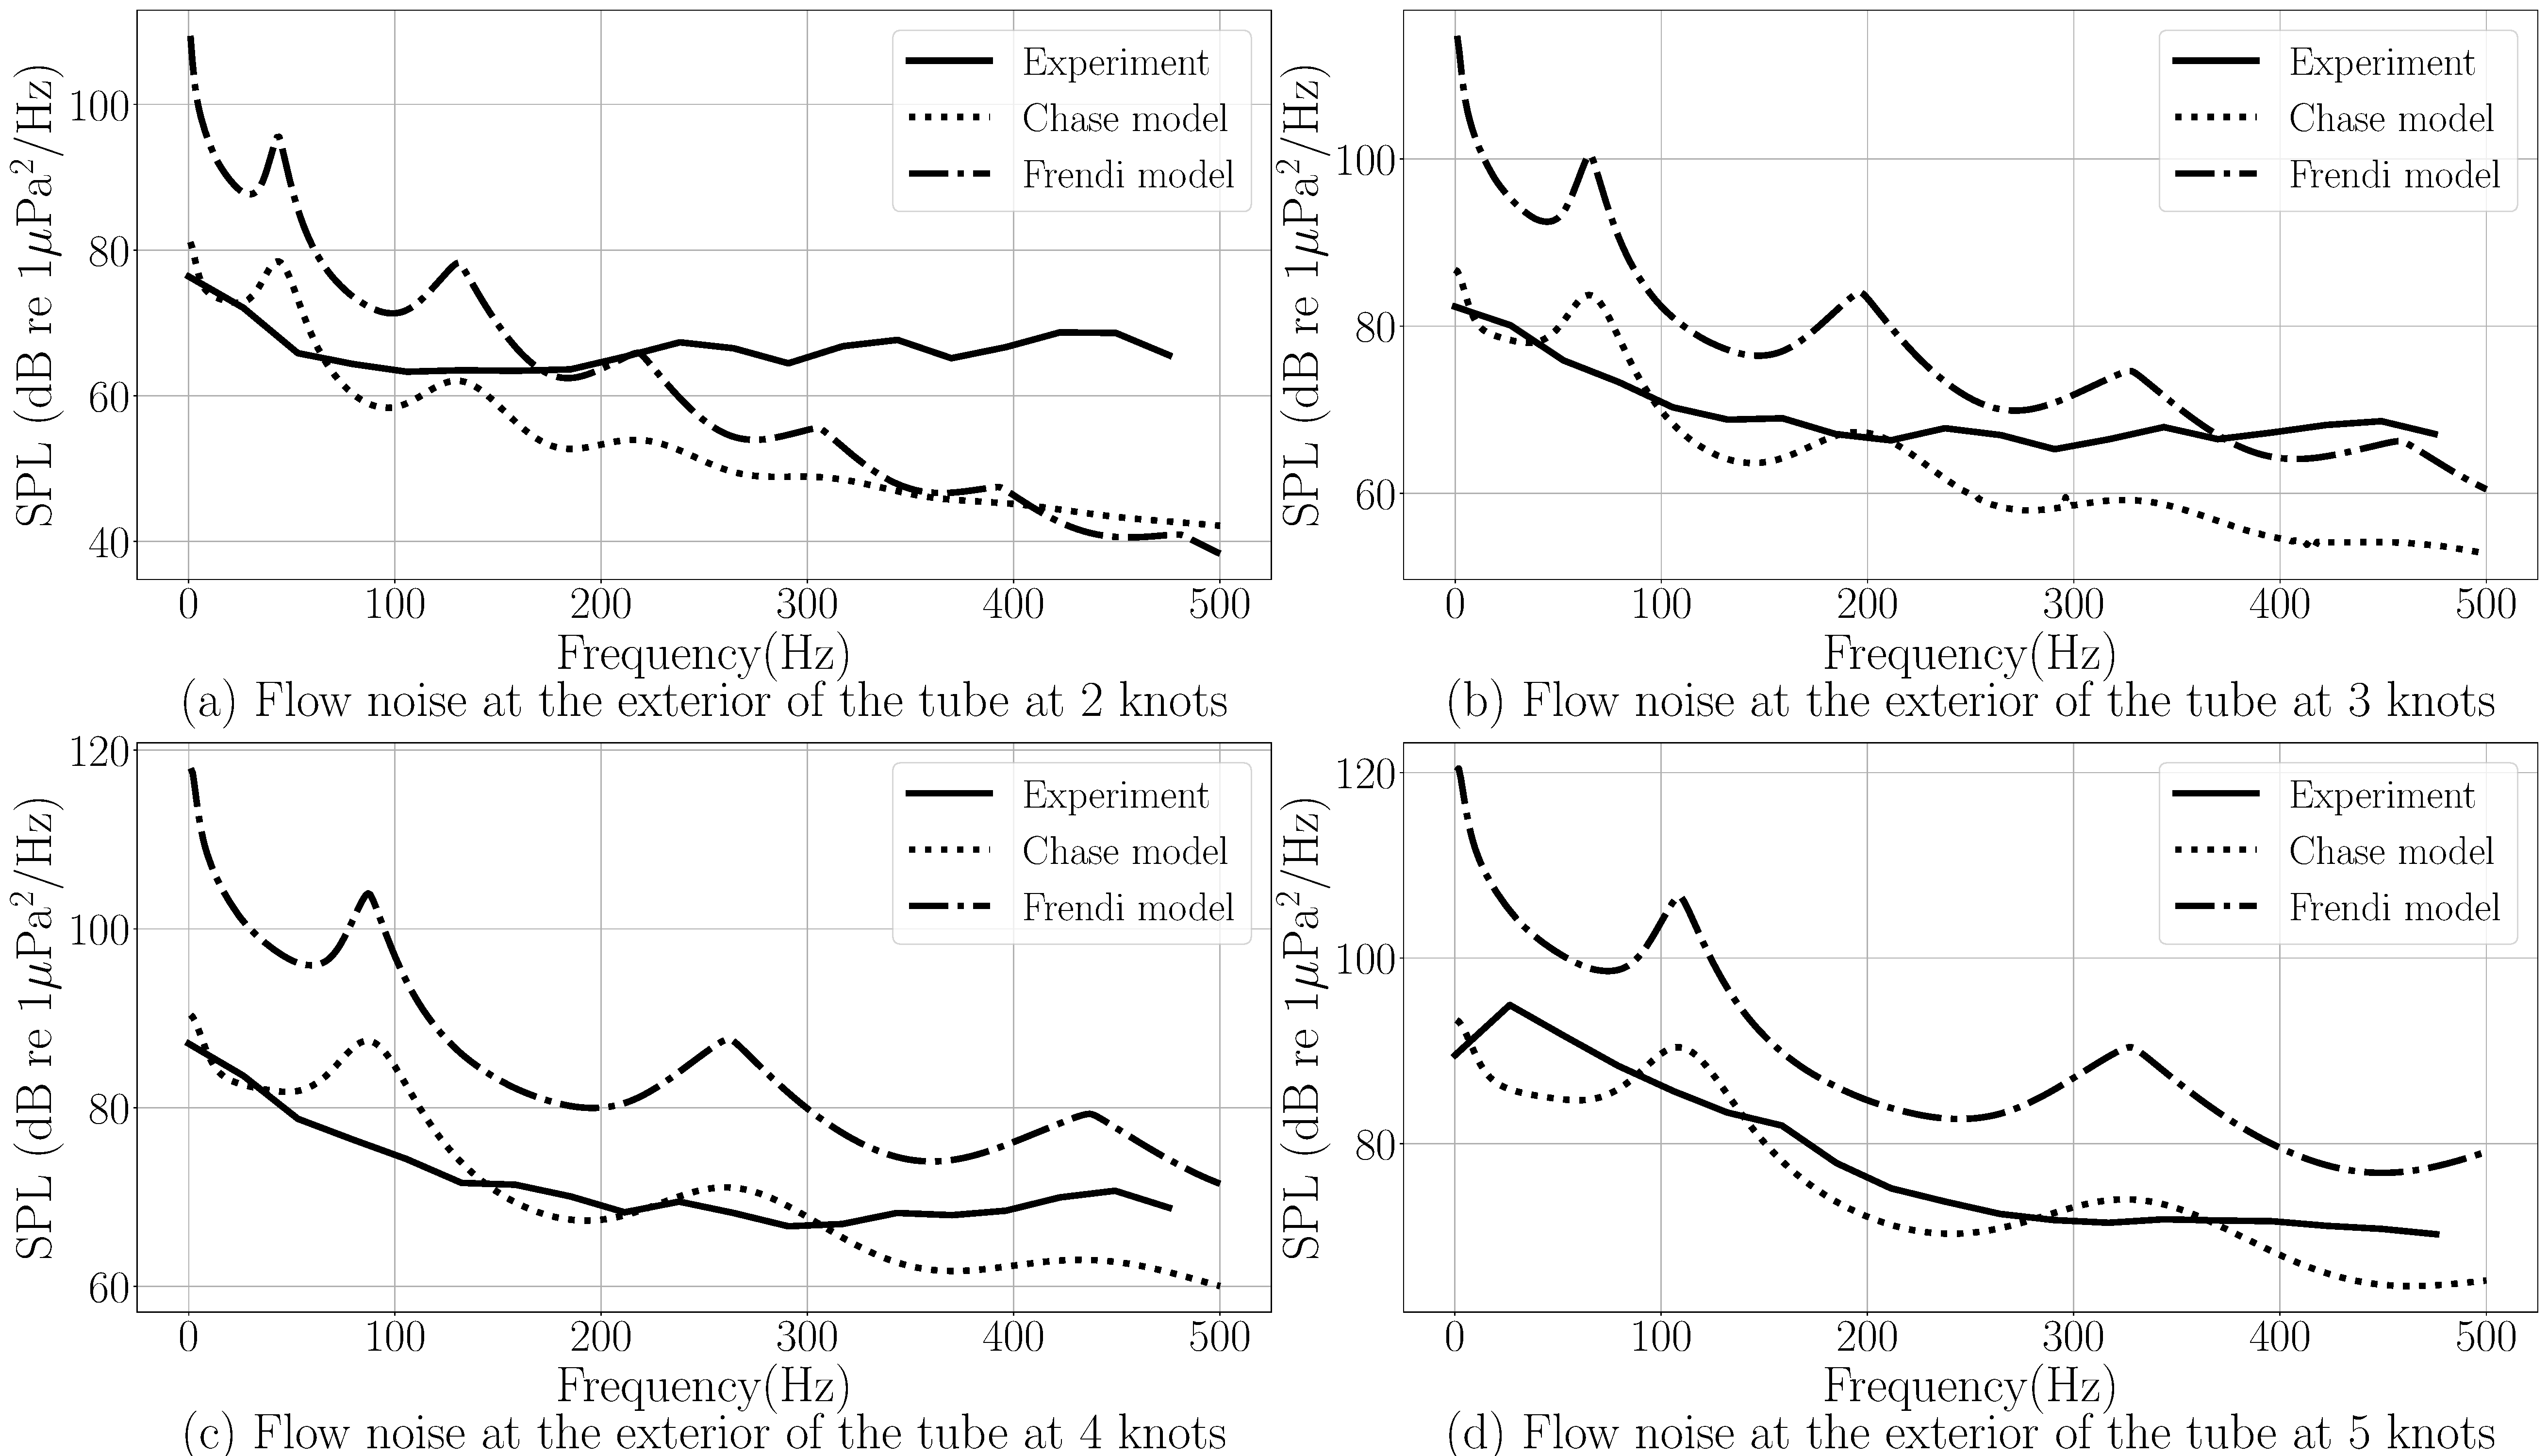
\includegraphics[width=3.1in]{figure/Chase ,frendi vs Unni comparison.pdf}
    \caption{Comparison of flow noise predicted by Chase~\cite{Chase1981} and Frendi~\cite{frendi2020} models with the experimental results~\cite{Unni2011} at different tow speeds.}
    \label{Chase,frendi,expt}
\end{figure}

Figure~\ref{Chase,frendi,expt} compares the flow noise estimated by the Chase~\cite{Chase1981} and Frendi~\cite{frendi2020} models with the experimental results~\cite{Unni2011} at various tow speeds for a solid cylinder having a diameter of 0.01~m. The sonar array consists of 66 hydrophones, each of length 8~mm, placed at the outer surface of the cylinder with an interval of 16~mm. It is evident from Fig.~\ref{Chase,frendi,expt} that the Frendi model consistently overestimates the flow noise at almost all frequencies and tow speeds, whereas the Chase model aligns well with experiments at high tow speeds. However, at low speeds, there is a significant difference between the Chase model and the experiment, especially at high frequencies. Regardless of tow speed, both the models predicts a significant reduction in the flow noise with frequency compared to the experimental results. To address these differences, a new model of turbulent pressure spectrum is proposed in this work to better match the experimental data, particularly at low tow speeds. The development of this new model is discussed in the following section.

\section{A new semi-empirical model of the turbulent pressure spectrum}\label{sec:hybmodel}
It is shown in the previous sections that the Chase and Frendi models show significant deviation from the experimental results~\cite{Unni2011} at low tow speeds and at high frequencies. In this section, a new semi-empirical model of the turbulent pressure spectrum is developed that closely aligns with the experimental results~\cite{Unni2011}. This new model is derived using the insights from both the Chase and the Frendi models, and is referred to as the \enquote{hybrid model}.

\subsection{The hybrid model}
In the \enquote{hybrid model}, the pressure spectrum from the Chase~\cite{Chase1981} model~(section.~\ref{Chase model}) is used in conjunction with the exponential decay function present in the Frendi~\cite{frendi2020} model~(section.~\ref{Frendi model}). Accordingly, the turbulent pressure spectrum is given by
\begin{equation}\label{hybrid model equation}
    \hat{p}(k_{z},k_{2},\omega) = C_{3}\Bar{P}(\omega)e^{-\hat{\alpha}r_{k}}.
\end{equation}
In the above equation, the autospectrum $\Bar{P}(\omega)$ is given by
\begin{equation}\label{autospectrum equation}
    \Bar{P}(\omega) = \int^{\infty}_{-\infty}\hat{p}_{0}(\omega,k_{z})dk_{z},
\end{equation}
where $\hat{p}_{0}(\omega,k_{z})$ is the same as that used in the Chase model~(Eq.~(\ref{Turbulent pressure spectrum equation Chase})). In this new model, the wavenumber dependency is included in the form of an exponential function $e^{-\hat{\alpha}r_{k}}$, where $\hat{\alpha} = \alpha\delta$ with
\begin{equation}\label{alpha hybrid model}
   \alpha = \frac{a_1}{\pi}\frac{1}{\sqrt{1+a_2(\frac{\omega \delta}{u_{t}}-50)^{2}}},
\end{equation}
\begin{equation}
    \delta = [48Re_a^{-1}Re_x^{(0.0226\log{Re_a}+0.2478)}]^{\frac{1}{0.91}}
\end{equation}
and
\begin{equation}
    |{r_{k}^{2}}| = (k_{z} - \frac{\omega}{u_{c}})^{2} + (mk_{2})^{2}.
\end{equation}
In Eq.~(\ref{alpha hybrid model}), $a_1$ and $a_2$ determine the behaviour of spectrum at low and high frequencies, respectively. It has been observed in Fig.~\ref{Chase,frendi,expt} that, the predictions of the Frendi model deviate more at higher frequency ranges. Therefore, the value of $a_2$ is decreased from $3\times10^{-5}$ to $3\times10^{-6}$. Different values of $a_1$ and $C_3$ were tested to match the experimental results given in Fig.~\ref{Chase,frendi,expt}. A better match is found with the experimental data when $a_1 = 1$ and $C_3=1\times10^{-4}$. Further, the turbulent pressure spectrum given in Eq.~(\ref{hybrid model equation}) is integrated over the cross-flow wavenumber $k_2$ from $-1/2R$ to $1/2R$~\cite{Chase1981} to obtain the pressure spectrum $\hat{p}_0(k_z,\omega)$ for axial flow past a solid cylinder. 
Thus,
\begin{equation}\label{hybrid model turbulent pressure}
    \hat{p}_0(k_{z},\omega) = \int_{-1/2R}^{1/2R}\hat{p}(k_{z},k_{2},\omega)dk_{2}.
\end{equation}

In the next section, the flow noise outside the cylinder is computed using the new hybrid model and the results are compared with existing models and Unnikrishnan's experimental results~\cite{Unni2011}.

\subsection{Flow noise}
The flow noise using the new hybrid model can be computed by Eq.~(\ref{Flow noise equaton from Unni}). Here, the hybrid model (Eqs.~(\ref{hybrid model equation})-(\ref{hybrid model turbulent pressure})) is used to compute the turbulent pressure spectrum $\hat{p}_0(k_z,\omega)$ and Eq.~(\ref{Hydrophone response equation from Unni}) is used for the hydrophone response function $H(k_z)$.


A comparison of flow noise measured in SPL (see Eq.~(\ref{SPL outside noise})) computed using the new hybrid model, Chase model~\cite{Chase1981} and Unnikrishnan's experiment~\cite{Unni2011} are shown in Fig.~\ref{fig:Flow_noise_of_Hybrid_model_with_chase_frendi_and_Unnikrishnan}. It can be seen that the new hybrid model's predictions match with the measured values~\cite{Unni2011} at all frequencies and towing speeds. Although, the hybrid model underpredicts noise at high frequencies for the 2 knots case, the predictions are better than that by the existing Chase and Frendi models.


A comparison of the turbulent pressure spectrum $\hat{p}_0(k_z,\omega)$ given by the hybrid model~(Eqs.~(\ref{hybrid model equation})-(\ref{hybrid model turbulent pressure})), the Chase model~(Eq.~(\ref{Turbulent pressure spectrum equation Chase})) and the Frendi model~(Eq.~(\ref{One D equation Frendi})) for a tow speed of 2 knots for different frequencies are shown in Fig.~\ref{pressure comparison of hybrid model with chase and Frendi}. The other parameters used to obtain the plot are the diameter of the cylinder which is chosen as 10~mm~\cite{Unni2011}, density of the fluid is 1000~kg/m$^3$ and the computation is done at 11~m from the leading edge of the solid cylinder. 
\begin{figure}[h]
    \centering
    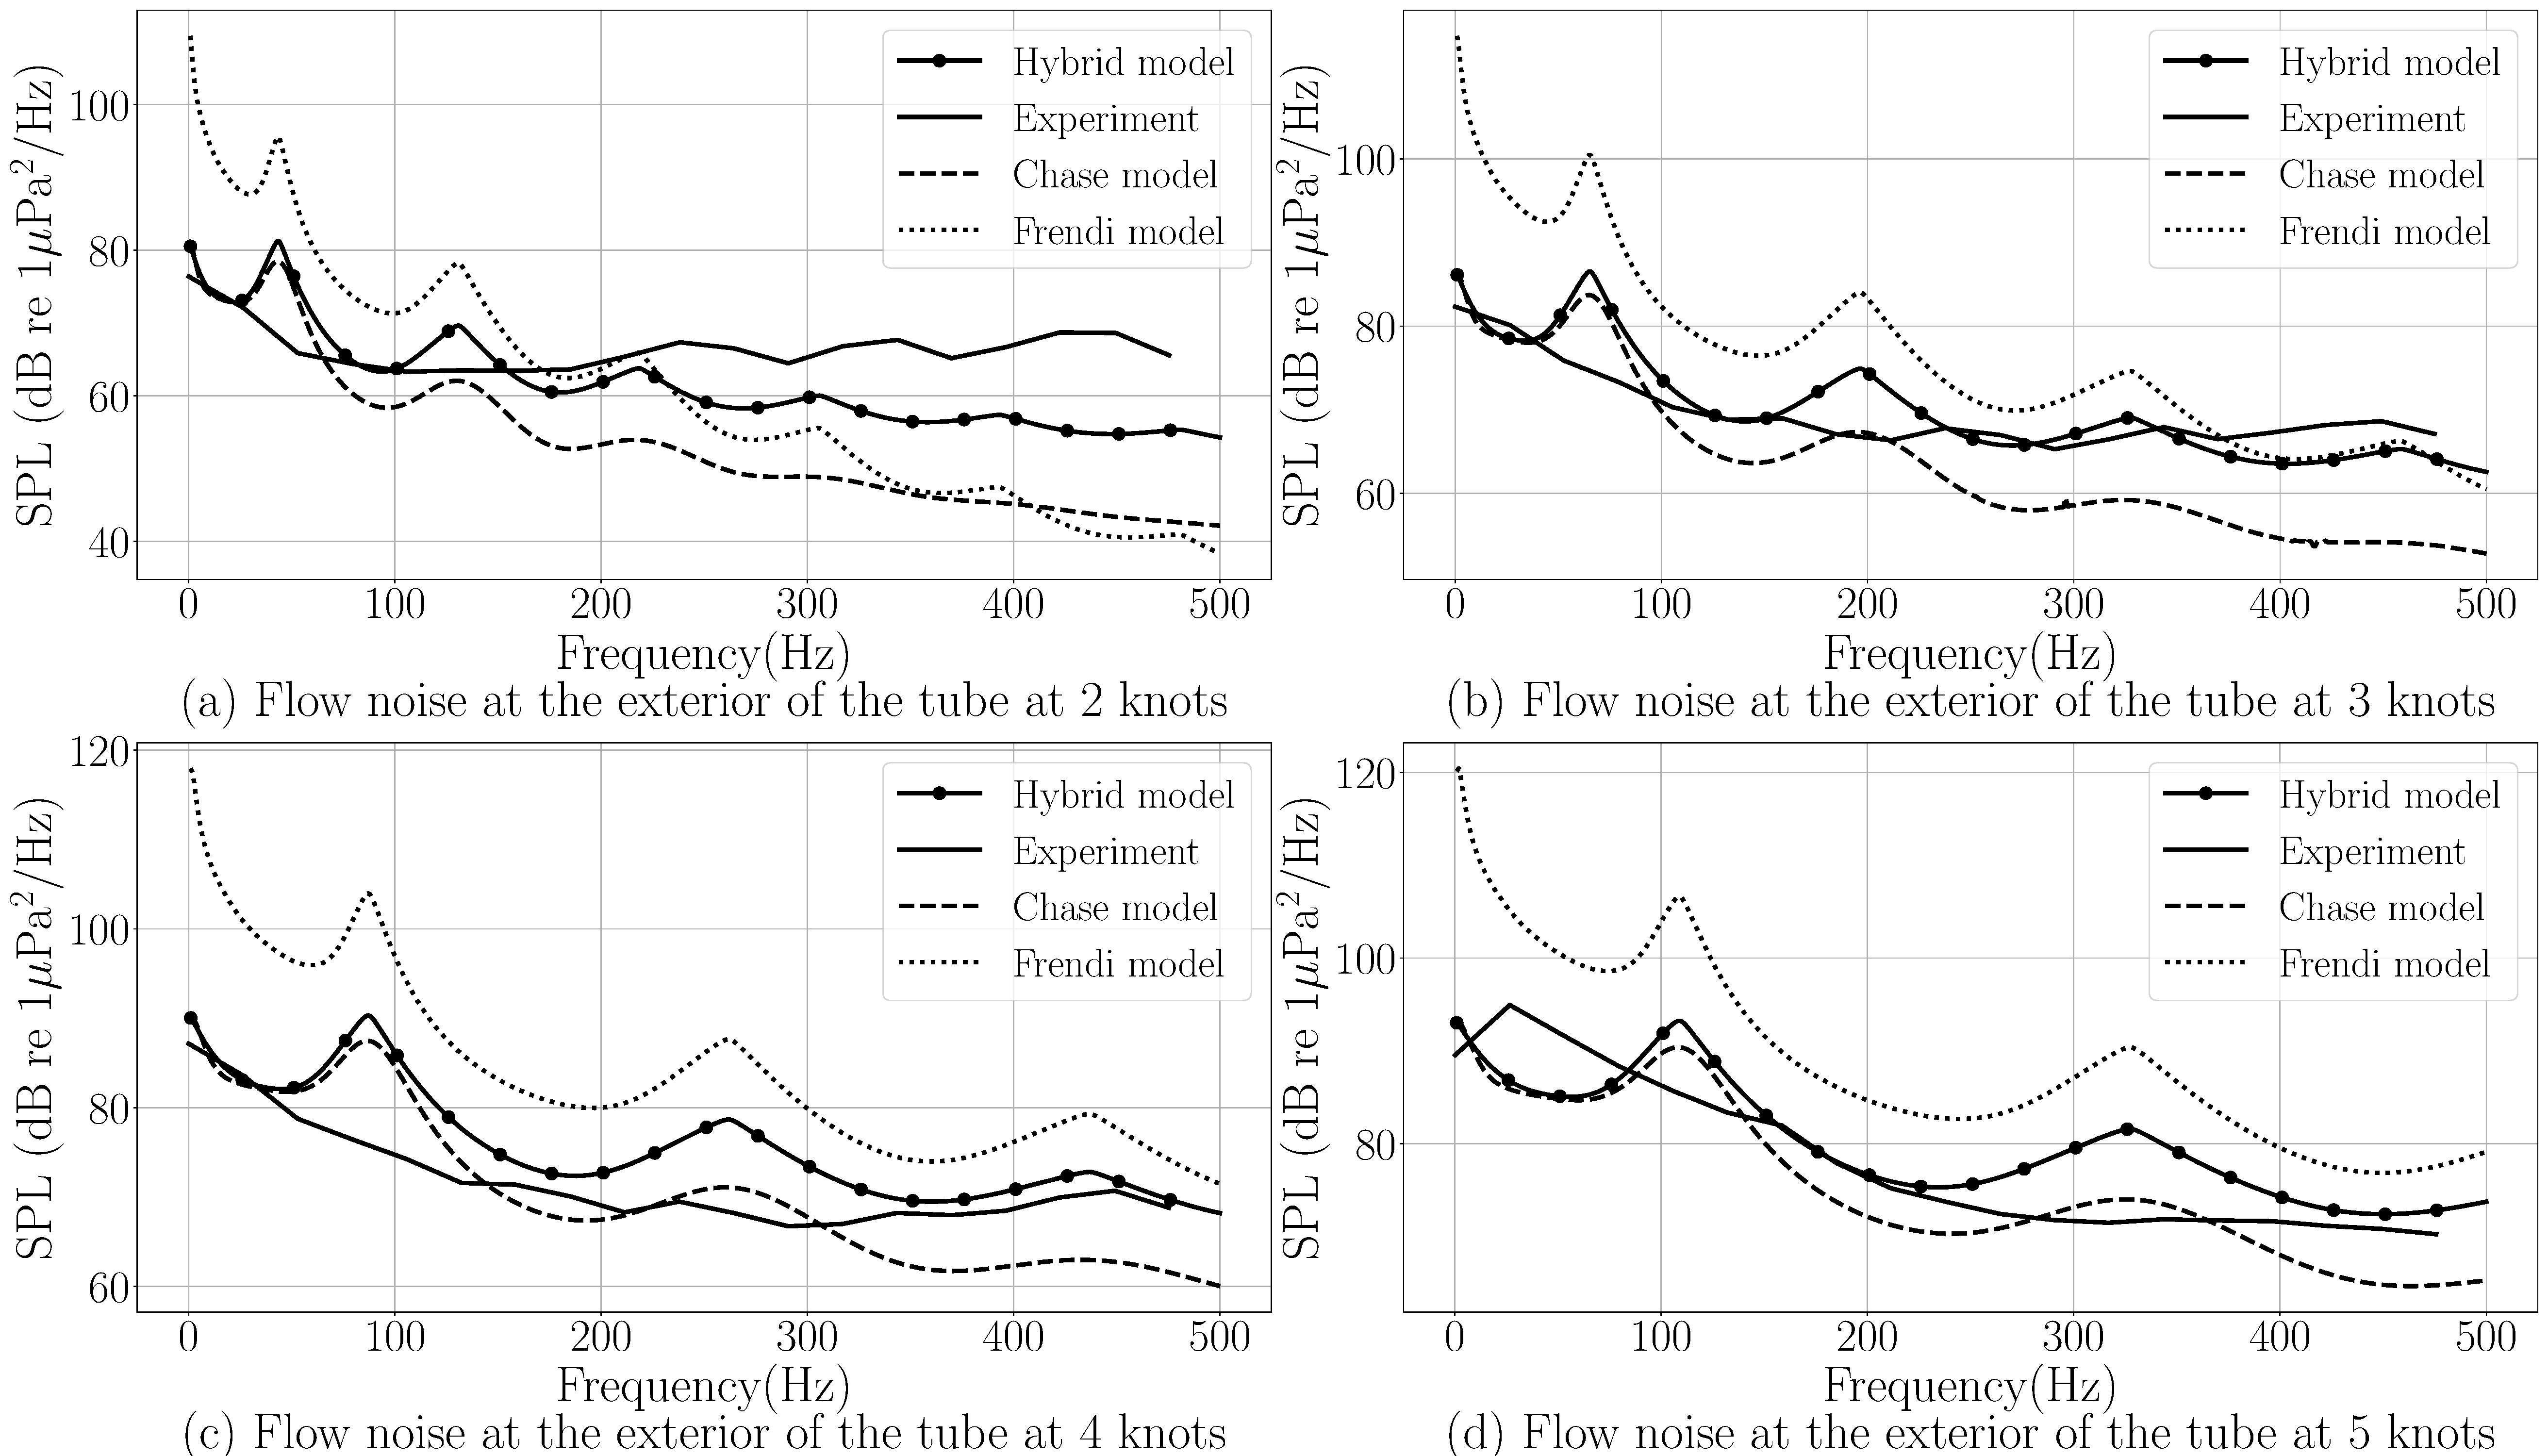
\includegraphics[width=3.1in]{figure/Hybrid_model_Chase_frendi_vs_Unni_comparison.pdf}
    \caption{A comparison of flow noise predicted by the hybrid model, the Chase model~\cite{Chase1981} and Frendi model~\cite{frendi2020} with that measured from experiments~\cite{Unni2011} at different tow speeds.}
    \label{fig:Flow_noise_of_Hybrid_model_with_chase_frendi_and_Unnikrishnan}
\end{figure}
\begin{figure}[h]
    \centering
    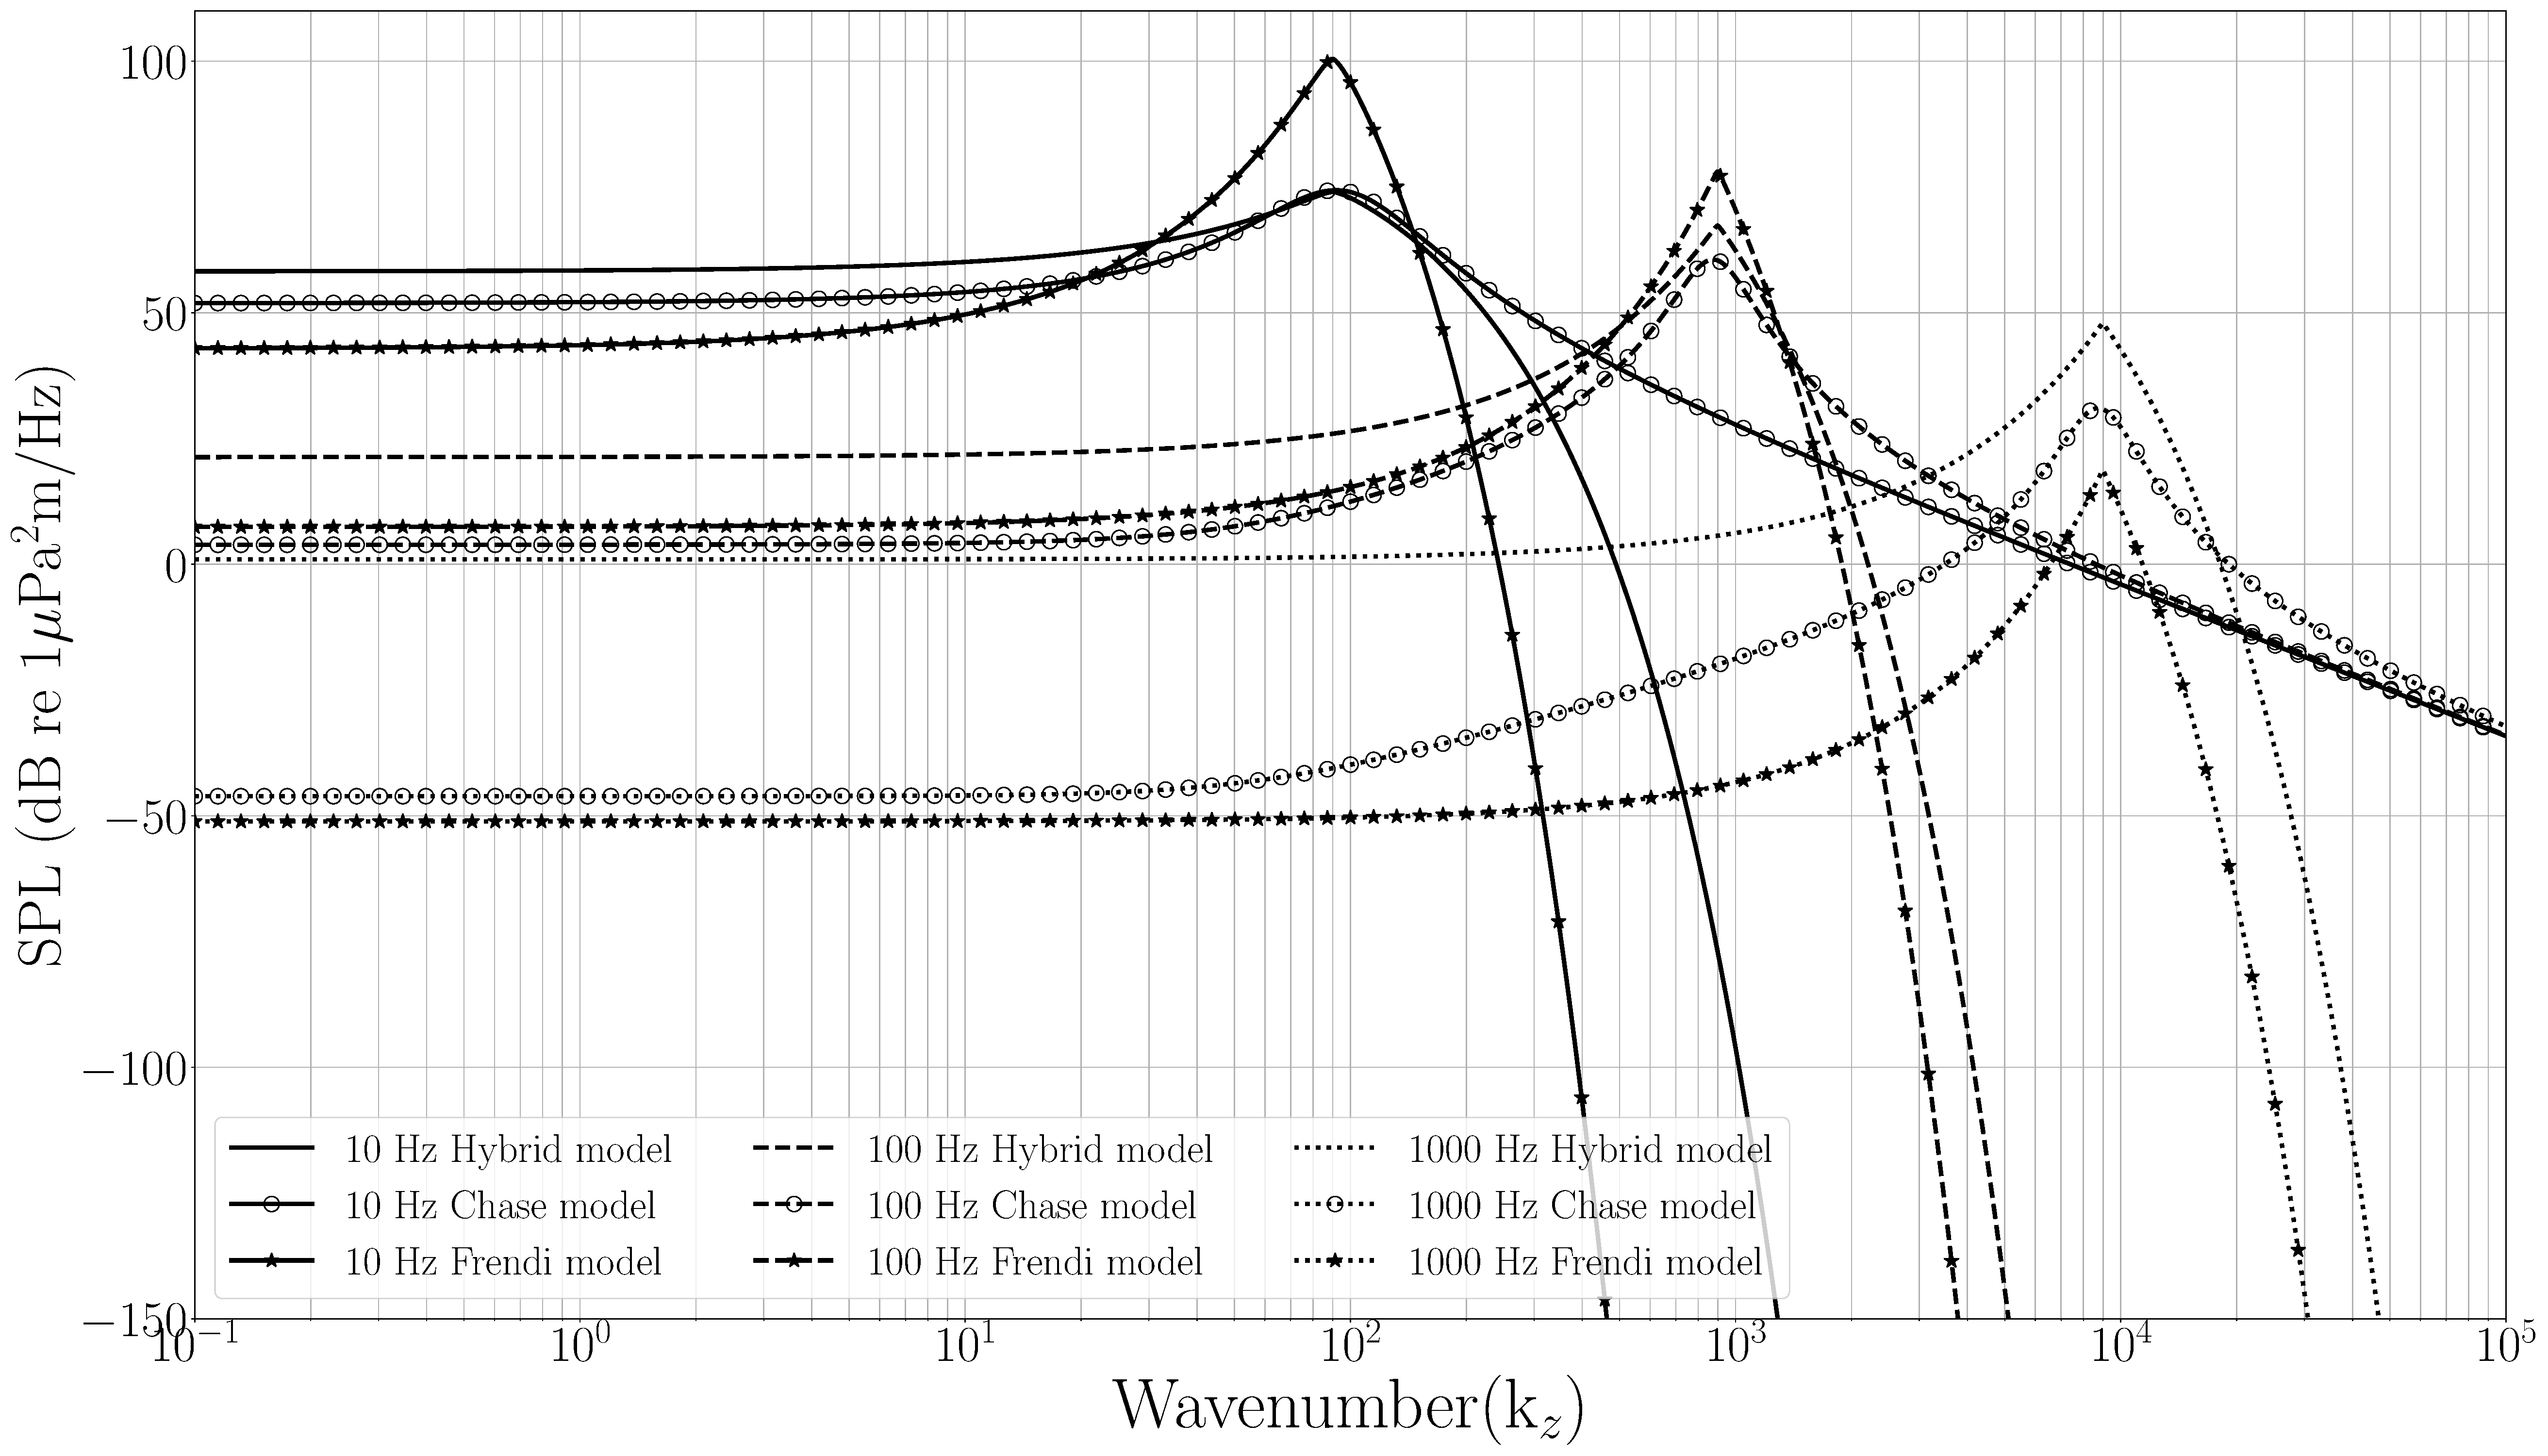
\includegraphics[width=3.1in]{figure/Chase_hybrid_Frendi_outside_pressure_Spectrum.pdf}
    \caption{A comparison of the turbulent pressure spectrum $\hat{p}_0(k_z,\omega)$ given by the hybrid model~(Eq.~(\ref{hybrid model turbulent pressure})), Chase~(Eq.~(\ref{Turbulent pressure spectrum equation Chase})) and Frendi~(Eq.~(\ref{One D equation Frendi})) model at 2~knots.}
    \label{pressure comparison of hybrid model with chase and Frendi}
\end{figure}
For a given frequency, at low wavenumbers, the turbulent pressure spectrum increases at a slow rate. It peaks at convective wavenumber $k_c$~($=\omega/u_c$) forming a convective ridge. It can be seen that while all the models predicts a `flat' spectrum at lower wavenumbers and a ridge at convective wavenumber, their predictions differ significantly at large wavenumbers. The presence of an exponential function results in an exponential decrease in the spectrum at large wavenumbers for the hybrid and Frendi models. Chase model predicts a higher spectrum with smaller slope at large wavenumbers. It can be seen from Fig.~\ref{pressure comparison of hybrid model with chase and Frendi} that the predictions by the three models are closer at lower frequencies. However, at high frequencies, the hybrid model predicts a higher spectrum than the rest. This difference in the spectrum predicted by the hybrid model helps to achieve a closer agreement with the measured flow noise as shown in Fig.~\ref{fig:Flow_noise_of_Hybrid_model_with_chase_frendi_and_Unnikrishnan}.

\subsection{Non-dimensional power spectral density}
The non-dimensional power spectral density, $Q_{ND}$, of flow noise is defined as
\begin{equation}
    Q_{ND} = \frac{Q(\omega)}{\rho^2 D U^3},
\end{equation}
where $Q(\omega)$ is the flow noise given by Eq.~(\ref{Flow noise equaton from Unni}) and $D$ is the cylinder diameter. The non-dimensional power spectral density calculated using the hybrid model Eqs.~(\ref{hybrid model equation})-(\ref{hybrid model turbulent pressure}) at different tow speeds are shown in Fig.~\ref{non dimensional plot of hybrid model}.
\begin{figure}[h]
    \centering
    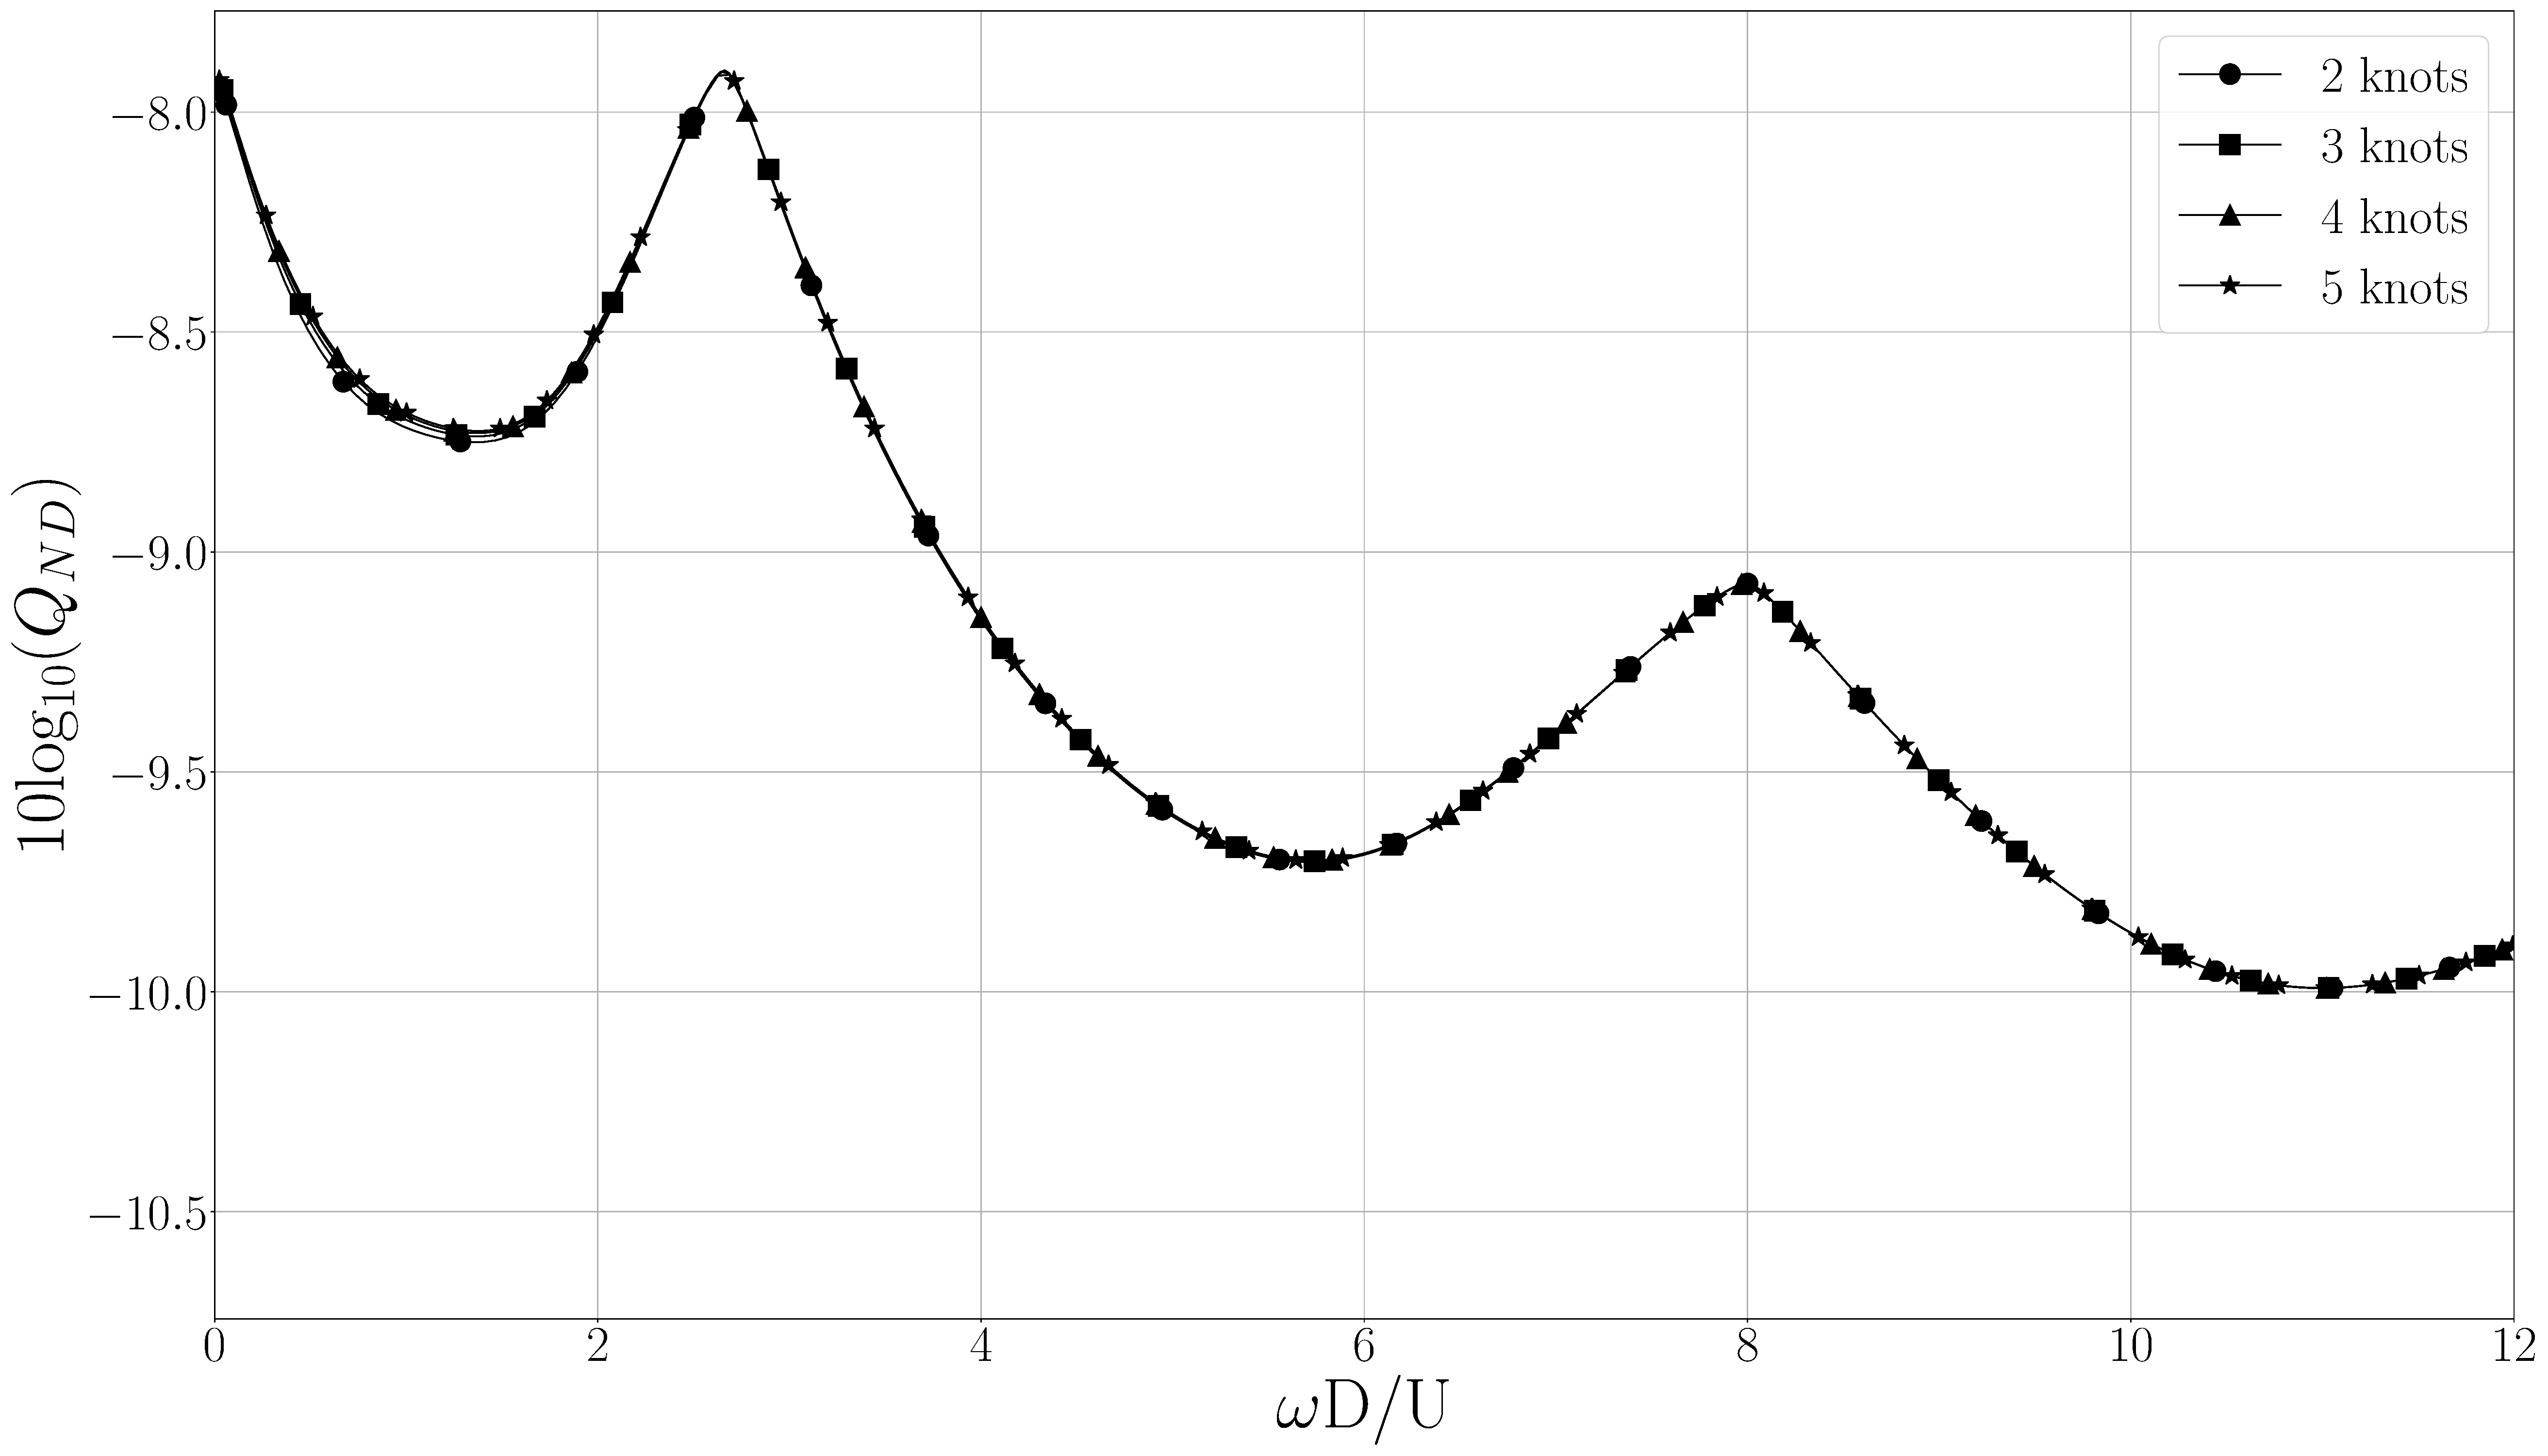
\includegraphics[width=3.1in]{figure/Non dimensional plot of hybrid model.pdf}
    \caption{Non-dimensional power spectral density for different tow speeds using the new hybrid model.}
    \label{non dimensional plot of hybrid model}
\end{figure}
It can be seen that, the non-dimensional power spectral density for different tow speeds collapse to a single curve against the non-dimensional frequency $\omega D/u$. One can obtain the power spectral density at different tow speeds and cylinder diameters using this \enquote{single} non-dimensional curve.


This section presented a new model of turbulent pressure field for axial flow past a solid cylinder and found that the model predictions are closer to an experimental results~\cite{Unni2011}. It was assumed that the cylinder is rigid and therefore the pressure field is not altered by the cylinder displacement field. However, the cylindrical tube in towed sonar arrays are not rigid and can be assumed to be elastic. The turbulent pressure fluctuation outside the elastic tube, creates vibration inside the tube and in turn generates acoustic waves in the fluid inside the tube. The next section presents a three-dimensional vibroacoustic model of a fluid-filled elastic tube, which is used in conjunction with the hybrid model for the external turbulent pressure excitation to estimate on-axis flow noise.


\section{Three-dimensional vibroacoustic model of a fluid-filled elastic tube} \label{sec:vamodel}
This section develops a fully coupled three-dimensional vibroacoustic model of the fluid-filled elastic tube. A schematic of fluid-filled tube is shown in Fig.~\ref{fig:fluid filled elastic tube}. First, the displacement field of the elastic tube is derived from the Navier-Lame equilibrium equation (see section.~\ref{governing equation for 3d cylinder}) and the acoustic pressure field inside the tube is derived from the acoustic wave equation (see section.~\ref{inside fluid modelling}). The structure (elastic tube) and the fluid (interior fluid) are then coupled with the help of stress and displacement boundary conditions at the interface (see section.~\ref{BCS}). The external pressure excitation is also accounted in the form of stress boundary condition at the outer surface of the tube. The boundary conditions, when expressed in terms of the unknown displacement and pressure fields, form a system of linear algebraic equations. The unknown displacement and pressure fields can be computed by solving this system of equations (see section.~\ref{solution methods}).

\begin{figure}
    \centering
    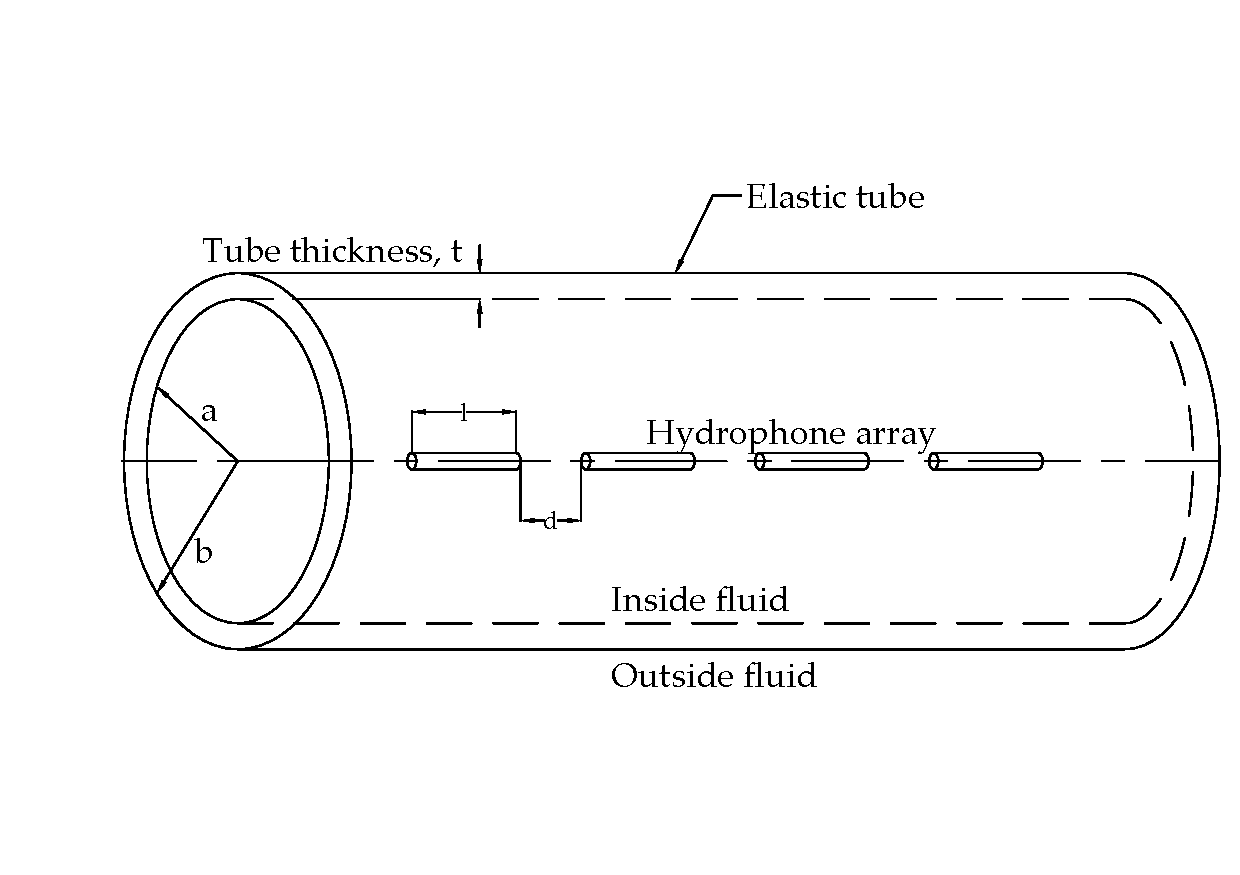
\includegraphics[width=3.1in]{figure/Sonar_array_element.pdf}
    \caption{Fluid filled elastic tube.}
    \label{fig:fluid filled elastic tube}
\end{figure}


\subsection{The elastic tube displacement and stress fields}\label{governing equation for 3d cylinder}
This section involves modelling of elastic tube using Navier-Lame's equilibrium equation~\cite{Martin2014} in three-dimensional cylindrical coordinates. The Navier-Lame equilibrium equation is given by
\begin{multline}\label{Navier equation of motion 3d}
    \mu\nabla^{2}\mathbf{U}(r,\theta,z,t)+(\lambda+\mu)\pmb{\nabla}\pmb{\nabla}.\mathbf{U}(r,\theta,z,t)\\ = \rho_s\mathbf{\ddot{U}}(r,\theta,z,t),
\end{multline}
where $\mathbf{U}$ is the displacement vector ($= \{W_e, \Theta_e, U_e\}^T$, $W_e$ represents the radial, $\Theta_e$ represents the azimuthal and $U_e$, the axial displacement field). $\lambda$ and $\mu$ are the Lame's coefficients, $\rho_s$ is the density of the tube and $\pmb{\nabla}$ is the gradient operator in three dimension given by
\begin{equation}\label{del operator}
    \pmb{\nabla} = \frac{\partial}{\partial r}{\mathbf{e_r}} + \frac{1}{r}\frac{\partial}{\partial \theta}\mathbf{e}_{\pmb{\theta}} + \frac{\partial}{\partial z}\mathbf{e_z}.
\end{equation}
The displacement vector $\mathbf{U}$ may be represented using the Helmholtz decomposition method as
 \begin{equation}\label{Helmholtz equation 3d}
    \mathbf{U} = \pmb{\nabla}\phi+\pmb{\nabla}\times\pmb{\psi},
\end{equation}
where $\phi$ is a scalar potential and $\pmb{\psi}$ is a vector potential. Substituting for $\mathbf{U}$ in Eq.~(\ref{Navier equation of motion 3d}) yields,
\begin{multline}
    \mu\nabla^{2}(\pmb{\nabla}\phi+\pmb{\nabla}\times\pmb{\psi})+(\lambda+\mu)\pmb{\nabla}\pmb{\nabla}.(\pmb{\nabla}\phi+\pmb{\nabla}\times\pmb{\psi})\\ = \rho_s\frac{\partial^{2}}{\partial t^{2}}(\pmb{\nabla}\phi+\pmb{\nabla}\times\pmb{\psi}).
\end{multline}
Rearranging the above equation, the obtained expression is,
\begin{multline}\label{NaLa simplified eqn}
    \pmb{\nabla}(\mu\nabla^{2}\phi+(\lambda+\mu)\nabla^{2}\phi-\rho_s\ddot{{\phi}})+\\ \pmb{\nabla}\times(\mu\nabla^{2}\pmb{\psi}-\rho_s\ddot{\pmb{\psi}}) = 0.
\end{multline}
Eq.~(\ref{NaLa simplified eqn}) may be separated to two equations each corresponding to the scalar and vector potential fields as,
\begin{equation*}
    (\lambda+2\mu)\nabla^{2}\phi-\rho_s\ddot{\phi} = 0 \hspace{1em} \text{and} \hspace{1em} \mu\nabla^{2}\pmb{\psi}-\rho_s\ddot{\pmb{\psi}} = 0.
\end{equation*}
The above equations are rearranged as,
\begin{equation}\label{Scalar potential Wave equation}
    \nabla^{2}\phi = \frac{1}{C_{L}^{2}}\ddot{\phi},
\end{equation}
where, $C_{L}^{2} = \frac{\lambda+2\mu}{\rho_s}$ and
\begin{equation}\label{Vector potential Wave equation}
    \nabla^{2}\pmb{\psi} = \frac{1}{C_{T}^{2}}\ddot{\pmb{\psi}},
\end{equation}
where, $C_{T}^{2} = \frac{\mu}{\rho_s}$.
Substituting for $\pmb{\psi} = \psi_r\mathbf{e}_r + \psi_\theta\mathbf{e}_\theta + \psi_z\mathbf{e}_z$ in Eq.~(\ref{Vector potential Wave equation}) results in~\cite{achenbach2012}
 \begin{equation}\label{Vector equation of r}
     \nabla^{2}\psi_{r}-\frac{\psi_{r}}{r^{2}}-\frac{2}{r^{2}}\frac{\partial\psi_{\theta}}{\partial\theta} = \frac{1}{C_T^{2}}\frac{\partial^{2}\psi_{r}}{\partial t^{2}},
 \end{equation}
  \begin{equation}\label{vector equation of theta}
     \nabla^{2}\psi_{\theta}-\frac{\psi_{\theta}}{r^{2}}-\frac{2}{r^{2}}\frac{\partial\psi_{r}}{\partial\theta} = \frac{1}{C_T^{2}}\frac{\partial^{2}\psi_{\theta}}{\partial t^{2}},
 \end{equation}
 and
 \begin{equation}\label{vector equation of z}
     \nabla^{2}\psi_{z}= \frac{1}{C_T^{2}}\frac{\partial^{2}\psi_{z}}{\partial t^{2}}.
 \end{equation}
The following subsections discuss the solution of the governing differential equations for the scalar potential function (Eq.~(\ref{Scalar potential Wave equation})) and the vector potential functions (Eqs.~(\ref{Vector equation of r}) - (\ref{vector equation of z})).

 \subsubsection{The scalar potential function $\phi$}
 A plane wave propagating in the positive $z$ direction can be written in the form
 \begin{equation}\label{Scalar potential Variable separable equation}
    \phi(r,\theta,z,t) = \Phi(r)\Theta(\theta)\mathbf{e}^{i(k_{z}z-\omega t)}.   
 \end{equation}
Subtituting Eq.~(\ref{Scalar potential Variable separable equation}) in  Eq.~(\ref{Scalar potential Wave equation}) and simplifying gives,
\begin{multline}
    \frac{r^{2}}{\Phi(r)}\frac{\partial^{2} \Phi(r)}{\partial r^{2}} + \frac{r}{\Phi(r)}\frac{\partial \Phi(r)}{\partial r} + r^2\bigg(\frac{\omega^{2}}{C_{L}^{2}}-k_{z}^{2}\bigg)\\ = -\frac{1}{\Theta(\theta)}\frac{\partial^{2} \Theta(\theta)}{\partial \theta^{2}}.
\end{multline}
The above equation is satisfied only if both the left and the right hand sides are equal to a constant, say $n^{2}$. Thus, the differential equations governing $\Phi(r)$ and $\Theta(\theta)$ can be separated as 
\begin{equation}\label{first part phi}
    \frac{\partial^{2} \Phi(r)}{\partial r^{2}} + \frac{1}{r}\frac{\partial \Phi(r)}{\partial r} + \left(\frac{\omega^{2}}{C_{L}^{2}}-k_{z}^{2} - \frac{n^{2}}{r^{2}}\right)\Phi(r) = 0
\end{equation}
and
\begin{equation}\label{second part phi}
    \frac{\partial^{2} \Theta(\theta)}{\partial \theta^{2}} + n^{2}\Theta(\theta) = 0.
\end{equation}
Eq.~(\ref{first part phi}) can be further simplified to 
\begin{equation}\label{bessel form scalar potential}
    \frac{d^{2}\Phi}{dr^{2}} + \frac{1}{r}\frac{d\Phi}{dr} + \left(\beta_1^{2} - \frac{n^{2}}{r^{2}}\right)\Phi = 0,
\end{equation}
where $\beta_1^{2} = \frac{\omega^{2}}{C_{L}^{2}} - k_z^{2}$. The solution of Eq.~(\ref{bessel form scalar potential}) is given by
\begin{equation}\label{Phi(R) for phi}
    \Phi(r) = A_{1}J_{n}(\beta_1 r) + A_{2}Y_{n}(\beta_1 r), 
\end{equation}
where $J_{n}$ and $Y_{n}$ are the Bessel function of the first and the second kinds of order $n$ respectively. The solution to Eq.~(\ref{second part phi}) can be derived as,
\begin{equation}\label{Theta(theta) for phi}
    \Theta(\theta) = A_{3}\cos(n\theta) + A_{4}\sin(n\theta).
\end{equation}
In Eqs.~(\ref{Phi(R) for phi}) and (\ref{Theta(theta) for phi}), $A_1$, $A_2$,$A_3$ and $A_4$ are the unknown constants. Substituting Eq.~(\ref{Phi(R) for phi}) and Eq.~(\ref{Theta(theta) for phi}) in to Eq.~(\ref{Scalar potential Variable separable equation}), the scalar potential function is given by
\begin{multline}\label{scalar potential function 1}
    \phi(r,\theta,z,t) = \left[A_{1}J_{n}(\beta_1 r) + A_{2}Y_{n}(\beta_1 r)\right]\times\\ \left[A_{3}\cos(n\theta) + A_{4}\sin(n\theta)\right]\mathbf{e}^{i(k_{z}z-\omega t)}.
\end{multline}
\subsubsection{The  vector potential function $\pmb{\psi}$}
It can be observed from Eqs.~(\ref{Vector equation of r})-(\ref{vector equation of theta}) that, both $\psi_r$ and $\psi_\theta$ are coupled and need to be solved simultaneously. However, Eq~(\ref{vector equation of z}) can be solved independently for $\psi_z$. Let $\psi_r$ and $\psi_\theta$ be of the form
\begin{equation}\label{Variable separable equation of r}
    \psi_{r}(r,\theta,z,t) = \Psi_{r}(r)\sin(n\theta)\mathbf{e}^{i(k_{z}z-\omega t)}
\end{equation}
and
\begin{equation}\label{Variable separable equation of theta}
    \psi_{\theta}(r,\theta,z,t) = \Psi_{\theta}(r)\cos(n\theta)\mathbf{e}^{i(k_{z}z-\omega t)}.
\end{equation}
Substituting Eq.~(\ref{Variable separable equation of r}) and Eq.~(\ref{Variable separable equation of theta}) in Eq.~(\ref{Vector equation of r}) and Eq.~(\ref{vector equation of theta}), respectively,
\begin{multline}\label{Differential equation of r}
    \frac{d^{2}\Psi_{r}}{dr^{2}} + \frac{1}{r}\frac{d\Psi_{r}}{dr} + \frac{1}{r^{2}}\left(-n^{2}\Psi_{r}+2n\Psi_{\theta}-\Psi_{r}\right)\\ - k_{z}^{2}\Psi_{r} + \frac{\omega^{2}}{C_{T}^{2}}\Psi_{r} = 0
\end{multline}
and 
\begin{multline}\label{Differential equation of theta}
    \frac{d^{2}\Psi_{\theta}}{dr^{2}} + \frac{1}{r}\frac{d\Psi_{\theta}}{dr} + \frac{1}{r^{2}}\left(-n^{2}\Psi_{\theta}+2n\Psi_{r}-\Psi_{\theta}\right)\\ - k_{z}^{2}\Psi_{\theta} + \frac{\omega^{2}}{C_{T}^{2}}\Psi_{\theta} = 0.
\end{multline}
Subtracting Eq.~(\ref{Differential equation of theta}) from Eq.~(\ref{Differential equation of r}),

\begin{multline}
    \frac{d^{2}(\Psi_{r}-\Psi_\theta)}{dr^{2}} + \frac{1}{r}\frac{d(\Psi_{r}-\Psi_\theta)}{dr}\\ + \frac{1}{r^{2}}\bigg(-n^{2}(\Psi_{r}-\Psi_\theta )+ 2n(\Psi_{\theta}-\Psi_r)-(\Psi_{r}-\Psi_\theta)\bigg)\\ - k_{z}^{2}(\Psi_{r}-\Psi_\theta) + \frac{\omega^{2}}{C_{T}^{2}}(\Psi_{r}-\Psi_\theta) = 0.
\end{multline}
Solving,
\begin{equation}\label{difference of r and theta}
    \Psi_{r} -\Psi_{\theta} = C_{1}J_{n+1}(\beta_2 r) + C_{2}Y_{n+1}(\beta_2 r),
\end{equation}
where $\beta_2^{2} = \frac{\omega^{2}}{C_{T}^{2}} - k_z^{2}$, $C_1$ and $C_2$ are unknown constants.
Adding Eqs.~(\ref{Differential equation of r}) and (\ref{Differential equation of theta}),
\begin{multline}
    \frac{d^{2}(\Psi_{r}+\Psi_\theta)}{dr^{2}} + \frac{1}{r}\frac{d(\Psi_{r}+\Psi_\theta)}{dr}\\ + \frac{1}{r^{2}}\bigg(-n^{2}(\Psi_{r}+\Psi_\theta )+ 2n(\Psi_{\theta}+\Psi_r)-(\Psi_{r}+\Psi_\theta)\bigg)\\ - k_{z}^{2}(\Psi_{r}+\Psi_\theta) + \frac{\omega^{2}}{C_{T}^{2}}(\Psi_{r}+\Psi_\theta) = 0.
\end{multline}
Solving,
\begin{equation}\label{sum of r and theta}
    \Psi_{r} + \Psi_{\theta} = D_{1}J_{n-1}(\beta_2 r) + D_{2}Y_{n-1}(\beta_2 r),
\end{equation}
where $D_1$ and $D_2$ are unknown constants. Using Eq.~(\ref{difference of r and theta}) and Eq.~(\ref{sum of r and theta}), $\Psi_{r}$ and $\Psi_{\theta}$ can be obtained as
\begin{multline}\label{simplified eqn vector r}
    \Psi_{r} = C_{1}J_{n+1}(\beta_2 r) + C_{2}Y_{n+1}(\beta_2 r)\\ + D_{1}J_{n-1}(\beta_2 r) + D_{2}Y_{n-1}(\beta_2 r) 
\end{multline}
and
\begin{multline}\label{simplified eqn vector theta}
    \Psi_{\theta} = D_{1}J_{n-1}(\beta_2 r) + D_{2}Y_{n-1}(\beta_2 r)\\- C_{1}J_{n+1}(\beta_2 r) - C_{2}Y_{n+1}(\beta_2 r).
\end{multline}
However, for vector potential function, $\pmb{\nabla}.\pmb{\psi} = 0$~\cite{achenbach2012}. This necessitates  $\Psi_{r} = -\Psi_{\theta}$. Therefore, using Eq.~(\ref{sum of r and theta}), $D1 = D2 = 0$. Thus,
\begin{equation}\label{Partial equation of r}
   \Psi_{r}(r) = C_{1}J_{n+1}(\beta_2 r) + C_{2}Y_{n+1}(\beta_2 r) 
\end{equation}
and 
\begin{equation}\label{Partial equation of theta}
    \Psi_{\theta}(\theta) = - C_{1}J_{n+1}(\beta_2 r) - C_{2}Y_{n+1}(\beta_2 r),
\end{equation}
Using the above equations, the radial~(Eq.~(\ref{Variable separable equation of r})) and azimuthal (Eq.~(\ref{Variable separable equation of theta})) components of the vector potential function are given by
\begin{multline}
    \psi_{r}(r,\theta,z,t) = \left[C_{1}J_{n+1}(\beta_2 r) + C_{2}Y_{n+1}(\beta_2 r)\right]\cdot \\ \sin(n\theta)\mathbf{e}^{i(k_{z}z-\omega t)}
\end{multline}
and
\begin{multline}
    \psi_{\theta}(r,\theta,z,t) = -\left[C_{1}J_{n+1}(\beta_2 r) + C_{2}Y_{n+1}(\beta_2 r)\right]\cdot \\ \cos(n\theta)\mathbf{e}^{i(k_{z}z-\omega t)}.
\end{multline}
The solution of the vector potential $\psi_{z}$ is similar to the solution of the scalar potential (Eq.~(\ref{scalar potential function 1})) which can be derived as,
\begin{multline}
   \psi_{z}(r,\theta,z,t) = \left[B_{1}J_{n}(\beta_2 r) + B_{2}Y_{n}(\beta_2r)\right]\cdot \\ \left[B_{3}\cos(n\theta) + B_{4}\sin(n\theta)\right]\mathbf{e}^{i(k_{z}z-\omega t)},
\end{multline}
The scalar and vector potential functions satisfy the Navier-Lame equation for $n=0$ and all positive integer values of $n$. Therefore, the complete solution to Navier-Lame equation can be obtained as
\begin{multline}\label{Scalar potential equation}
    \phi(r,\theta,z,t) = \sum_{n=0}^{\infty}\left[A_{1}J_{n}(\beta_1 r) + A_{2}Y_{n}(\beta_1 r)\right]\cdot\\ \left[A_{3}\cos(n\theta) + A_{4}\sin(n\theta)\right]\mathbf{e}^{i(k_{z}z-\omega t)},
\end{multline}
\begin{multline}\label{Vector potential equation r}
    \psi_{r}(r,\theta,z,t) = \sum_{n=0}^{\infty}\left[C_{1}J_{n+1}(\beta_2r) + C_{2}Y_{n+1}(\beta_2 r)\right]\cdot\\ \sin(n\theta)\mathbf{e}^{i(k_{z}z-\omega t)},
\end{multline}
\begin{multline}\label{Vector potential equation theta}
    \psi_{\theta}(r,\theta,z,t) = \sum_{n=0}^{\infty}-\left[C_{1}J_{n+1}(\beta_2 r) + C_{2}Y_{n+1}(\beta_2 r)\right]\cdot\\ \cos(n\theta)\mathbf{e}^{i(k_{z}z-\omega t)}
\end{multline}
and
\begin{multline}\label{Vector potential equation z}
    \psi_{z}(r,\theta,z,t) = \sum_{n=0}^{\infty}\left[B_{1}J_{n}(\beta_2 r) + B_{2}Y_{n}(\beta_2 r)\right]\cdot\\ \left[B_{3}\cos(n\theta) + B_{4}\sin(n\theta)\right]\mathbf{e}^{i(k_{z}z-\omega t)}
\end{multline}
In this work, the above expressions are truncated to only $n=0$ and $n=1$ terms and further used to compute the elastic tube displacement and stress fields.

\subsubsection{Elastic tube displacement components}
In this subsection, the displacement components of the elastic tube in radial ($W_e$), azimuthal ($\Theta_e$) and axial ($U_e$) directions, are derived using the potential functions derived in the previous subsection. Using Eq.~(\ref{Helmholtz equation 3d}), the displacement components are
\begin{equation}
    W_{e}(r,\theta,z,t) = \frac{\partial\phi}{\partial r} + \frac{1}{r}\frac{\partial\psi_{z}}{\partial\theta} - \frac{\partial\psi_{\theta}}{\partial z},
\end{equation}
\begin{equation}
    \Theta_e(r,\theta,z,t) = \frac{1}{r}\frac{\partial\phi}{\partial\theta} + \frac{\partial\psi_r}{\partial z} - \frac{\partial\psi_z}{\partial r}
\end{equation}
and
\begin{equation}
    U_{e}(r,\theta,z,t) = \frac{\partial\phi}{\partial r} + \frac{1}{r}\frac{\partial\psi_{z}}{\partial\theta} - \frac{\partial\psi_{\theta}}{\partial z}
\end{equation}
Substituting for the scalar (Eq.~(\ref{Scalar potential equation})) and the vector potential (Eqs.~(\ref{Vector potential equation r}) - (\ref{Vector potential equation z})) functions,
\begin{multline}
    W_e(r,\theta,z,t) = \mathbf{e}^{i(k_{z}z-\omega t)}\bigg\{\frac{1}{r}[r\beta_1 J_0(r\beta_1)\cos(\theta)\\ - J_1(r\beta_1)(\cos(\theta) + r\beta_1)]E_1\\ + \frac{1}{r}\sin(\theta)[r\beta_1 J_0(r\beta_1) - J_1(r\beta_1)]E_2\\ + \frac{1}{r}[r\beta_1 Y_0(r\beta_1)\cos(\theta) - Y_1(r\beta_1)(\cos(\theta) + r\beta_1)]F_1\\ + \frac{1}{r}\sin(\theta)[r\beta_1 Y_0(r\beta_1) - Y_1(r\beta_1)]F_2\\ + ik_z[J_1(r\beta_2) + J_2(r\beta_2)\cos(\theta)]G_1\\ + ik_z[J_1(r\beta_2) + J_2(r\beta_2)\cos(\theta)]G_2\\ + [\frac{1}{r}J_1(r\beta_2)\cos(\theta)]H_1 + [\frac{1}{r}Y_1(r\beta_2)\cos(\theta)]H_2\\ - [\frac{1}{r}J_1(r\beta_2)\sin(\theta)]I_1 - [\frac{1}{r}Y_1(r\beta_2)\sin(\theta)]I_2 \bigg\},
\end{multline}
where, $E_1$, $E_2$, $F_1$, $F_2$, $G_1$, $G_2$, $H_1$, $H_2$, $I_1$ and $I_2$ are unknown constants with $E_1 = A_1A_3$, $E_2 = A_1A_4$, $F_1 = A_2A_3$, $F_2 = A_2A_4$, $G_1 = C_1$, $G_2 = C_2$, $H_1 = B_1B_4$, $H_2 = B_2B_4$, $I_1 = B_1B_3$ and $I_2 = B_2B_3$,
\begin{multline}
    \Theta_e(r,\theta,z,t) = \mathbf{e}^{i(k_{z}z-\omega t)}\bigg\{\frac{-1}{r}[J_1(r\beta_1)\sin(\theta)]E_1\\ + \frac{1}{r}[J_1(r\beta_1)\cos(\theta)]E_2 + \frac{-1}{r}[Y_1(r\beta_1)\sin(\theta)]F_1\\ + \frac{1}{r}[Y_1(r\beta_1)\cos(\theta)]F_2 + [ik_zJ_2(r\beta_2)\sin(\theta)]G_1\\ + [ik_zY_2(r\beta_2)\sin(\theta)]G_2\\ - \frac{\beta_2\sin(\theta)}{2}[J_0(r\beta_2)-J_2(r\beta_2)]H_1\\ - \frac{\beta_2\sin(\theta)}{2}[Y_0(r\beta_2)-Y_2(r\beta_2)]H_2\\ + \frac{1}{r}\{-r\beta_2J_0(r\beta_2)\cos(\theta) + J_1(r\beta_2)[r\beta_2+\cos(\theta)]\}I_1\\ + \frac{1}{r}\{-r\beta_2Y_0(r\beta_2)\cos(\theta) + Y_1(r\beta_2)[r\beta_2+\cos(\theta)]\}I_1\bigg\}
\end{multline}
and
\begin{multline}
    U_e(r,\theta,z,t)\\ = \mathbf{e}^{i(k_{z}z-\omega t)}\bigg\{ik_z[J_{0}(r\beta_1) + J_{1}(r\beta_1)\cos(\theta)]E_1\\ + [ik_zJ_{1}(r\beta_1)\sin(\theta)]E_2 +  ik_z[Y_{0}(r\beta_1) + Y_{1}(r\beta_1)\cos(\theta)]F_1\\ +[ik_zY_{1}(r\beta_1)\sin(\theta)]F_2 
    - \beta_2[J_{0}(r\beta_2) + J_{1}(r\beta_2)\cos(\theta)]G_1\\ - \beta_2[Y_{0}(r\beta_2) + Y_{1}(r\beta_2)\cos(\theta)]G_2\bigg\}.
\end{multline}
The spatio-temporal ($r, \theta, z, t$) displacement is then transformed to the wavenumber-frequency ($r, \theta, k_z, \omega$) domain using the Fourier transform pairs,
\begin{multline}\label{Forward fourier transform}
    \hat{G}(r,\theta,k_{z},\omega)\\ = \frac{1}{4\pi^{2}}\int^{\infty}_{-\infty}\int^{\infty}_{-\infty}g(r,\theta,z,t)e^{-i(k_{z}z-\omega t)}dzdt,
\end{multline}
and
\begin{multline}\label{Backward fourier transform}
    g(r,\theta,z,t)\\ = \int^{\infty}_{-\infty}\int^{\infty}_{-\infty}\hat{G}(r,\theta,k_{z},\omega)\mathbf{e}^{i(k_{z}z-\omega t)}dk_{z}d\omega.
\end{multline} 
The transformed displacement components are given below,
\begin{enumerate}[label=\roman*]
    \item Radial displacement,
    \begin{multline}\label{Radial displacement 3d}
    \hat{W}_{e}(r,\theta,k_z,\omega) =\\ \Bigg\{\frac{-\chi_1}{2}\{2J_1(r\beta_1) + [J_2(r\beta_1)\\ - J_0(r\beta_1)]\cos(\theta)\}\Bigg\}\hat{P}_1(k_z,\omega)\\ + \Bigg\{\frac{\chi_1}{2}[J_0(r\beta_1) - J_2(r\beta1)]\sin(\theta)\Bigg\}\hat{P}_2(k_z,\omega)\\ + \Bigg\{\frac{-\chi_1}{2}\{2Y_1(r\beta_1) + [Y_2(r\beta_1)\\-Y_0(r\beta_1)]\cos(\theta)\}\Bigg\}\hat{Q}_1(k_z,\omega)\\ + \Bigg\{\frac{\chi_1}{2}[Y_0(r\beta_1)-Y_2(r\beta1)]\sin(\theta)\Bigg\}\hat{Q}_2(k_z,\omega)\\ - \Bigg\{\chi_2[J_1(r\beta_2)+J_2(r\beta_2)\cos(\theta)]\Bigg\}\hat{R}_1(k_z,\omega)\\ - \Bigg\{\chi_2[Y_1(r\beta_2) + Y_2(r\beta_2)\cos(\theta)]\Bigg\}\hat{R}_2(k_z,\omega)\\ + \Bigg\{\frac{1}{r}[J_1(r\beta_2)\cos(\theta)]\Bigg\}\hat{S}_1(k_z,\omega)\\ + \Bigg\{\frac{1}{r}[Y_1(r\beta_2)\cos(\theta)]\Bigg\}\hat{S}_2(k_z,\omega)\\ + \Bigg\{\frac{1}{r}[J_1(r\beta_2)\sin(\theta)]\Bigg\}\hat{T}_1(k_z,\omega)\\ + \Bigg\{\frac{1}{r}[Y_1(r\beta_2)\sin(\theta)]\Bigg\}\hat{T}_2(k_z,\omega),
    \end{multline}
	
    where $\hat{P}_1(k_z,\omega)$, $\hat{P}_2(k_z,\omega)$, $\hat{Q}_1(k_z,\omega)$, $\hat{Q}_2(k_z,\omega)$, $\hat{R}_1(k_z,\omega)$, $\hat{R}_2(k_z,\omega)$, $\hat{S}_1(k_z,\omega)$, $\hat{S}_2(k_z,\omega)$, $\hat{T}_1(k_z,\omega)$ and $\hat{T}_2(k_z,\omega)$ are the unknown variables and $\chi_{1} = \frac{\beta_1}{jk_z}$ and $\chi_{2} =\frac{jk_z}{\beta_2}$.
	
    \item Azimuthal displacement,
    \begin{multline}\label{Azimuthal displacement 3d}
    \hat{\Theta}_e(r,\theta,k_z,\omega) =\\ \Bigg\{\frac{-\chi_1}{r\beta_1}[J_1(r\beta_1)\sin(\theta)]\Bigg\}\hat{P}_1(k_z,\omega)\\ + \Bigg\{\frac{\chi_1}{r\beta_1}[J_1(r\beta_1)\cos(\theta)]\Bigg\}\hat{P}_2(k_z,\omega)\\ + \Bigg\{\frac{-\chi_1}{r\beta_1}[Y_1(r\beta_1)\sin(\theta)]\Bigg\}\hat{Q}_1(k_z,\omega)\\ + \Bigg\{\frac{\chi_1}{r\beta_1}[Y_1(r\beta_1)\cos(\theta)]\Bigg\}\hat{Q}_2(k_z,\omega)\\ - \Bigg\{\chi_2J_2(r\beta_2)\sin(\theta)\Bigg\}\hat{R}_1(k_z,\omega)\\ - \Bigg\{\chi_2Y_2(r\beta_2)\sin(\theta)\Bigg\}\hat{R}_2(k_z,\omega)\\ + \Bigg\{\frac{\sin(\theta)}{r}[J_1(r\beta_2)-r\beta_2J_0(r\beta_2)]\Bigg\}\hat{S}_1(k_z,\omega)\\ + \Bigg\{\frac{\sin(\theta)}{r}[Y_1(r\beta_2)-r\beta_2Y_0(r\beta_2)]\Bigg\}\hat{S}_2(k_z,\omega)\\ + \Bigg\{\beta_2J_0(r\beta_2)\cos(\theta)\\-\frac{1}{r}\{J_1(r\beta_2)*[r\beta_2+\cos(\theta)]\}\Bigg\}\hat{T}_1(k_z,\omega)\\ + \Bigg\{\beta_2Y_0(r\beta_2)\cos(\theta)\\-\frac{1}{r}\{Y_1(r\beta_2)*[r\beta_2+\cos(\theta)]\}\Bigg\}\hat{T}_2(k_z,\omega)
    \end{multline}
and
    \item Axial displacement,
    \begin{multline}\label{Axial displacement 3d}    
    \hat{U}_{e}(r,\theta,k_z,\omega) =\\ \bigg\{J_{0}(r\beta_1) + J_{1}(r\beta_1)\cos(\theta)\bigg\}\hat{P}_1(k_z,\omega)\\ + \bigg\{J_{1}(r\beta_1)\sin(\theta)\bigg\}\hat{P}_2(k_z,\omega)\\
    + \bigg\{Y_{0}(r\beta_1) + Y_{1}(r\beta_1)\cos(\theta)\bigg\}\hat{Q}_1(k_z,\omega)\\ + \bigg\{Y_{1}(r\beta_1)\sin(\theta)\bigg\}\hat{Q}_2(k_z,\omega)\\
    + \bigg\{J_{0}(r\beta_2) + J_{1}(r\beta_2)\cos(\theta)\bigg\}\hat{R}_1(k_z,\omega)\\ + \bigg\{Y_{0}(r\beta_2) + Y_{1}(r\beta_2)\cos(\theta)\bigg\}\hat{R}_2(k_z,\omega).
    \end{multline}    
\end{enumerate}
The unknown variables in the displacement components, are related to the unknown constants $A_1$, $A_2$, $A_3$, $A_4$, $B_1$, $B_2$, $B_3$, $B_4$, $C_1$ and $C_2$ in the potential functions as,
\begin{align}\label{P unknown with A}
    \hat{P}_1(k_z,\omega) = 2\pi i A_1 A_3 k_z\delta(k+k_z)\delta(\omega-\omega_0),\\\hat{P}_2(k_z,\omega) = 2\pi i A_2 A_3 k_z\delta(k+k_z)\delta(\omega-\omega_0),
\end{align}
\begin{align}\label{Q unknown with A}
    \hat{Q}_1(k_z,\omega) = 2\pi i A_1 A_4 k_z\delta(k+k_z)\delta(\omega-\omega_0),\\\hat{Q}_2(k_z,\omega) = 2\pi i A_2 A_4 k_z\delta(k+k_z)\delta(\omega-\omega_0),
\end{align}
\begin{align}\label{R unknown with C}
    \hat{R}_1(k_z,\omega) = -2\pi C_1\beta_1\delta(k+k_z)\delta(\omega-\omega_0),\\\hat{R}_2(k_z,\omega) = -2\pi C_2\beta_1\delta(k+k_z)\delta(\omega-\omega_0),
\end{align}
\begin{align}\label{S unknown with B}
    \hat{S}_1(k_z,\omega) = 2\pi B_1 B_4\delta(k+k_z)\delta(\omega-\omega_0),\\ \hat{S}_2(k_z,\omega) = 2\pi B_2 B_4\delta(k+k_z)\delta(\omega-\omega_0),
\end{align}
\begin{align}\label{T unknown with B}
    \hat{T}_1(k_z,\omega) = -2\pi B_1 B_3\delta(k+k_z)\delta(\omega-\omega_0),\\ \hat{T}_2(k_z,\omega) = -2\pi B_2 B_3\delta(k+k_z)\delta(\omega-\omega_0)\label{T unknown with B2},
\end{align}
where $\delta$ is the dirac delta function.~From the above equations (Eqs.~(\ref{P unknown with A})-(\ref{T unknown with B2})), two unknown variables can be expressed in terms of other variables as,
\begin{multline}\label{relation between constants}
    \hat{Q}_2(k_z,\omega) = \frac{\hat{P}_2(k_z,\omega) \hat{Q}_1(k_z,\omega)}{\hat{P}_1(k_z,\omega)},\\ \hat{T}_2(k_z,\omega) = \frac{\hat{S}_2(k_z,\omega) \hat{T}_1(k_z,\omega)}{\hat{S}_1(k_z,\omega)}.
\end{multline}
From the displacement components derived in this section, there are ten unknown variables, out of which only eight are independent (Eq.~(\ref{relation between constants})). Further, using the displacement components, normal and shear stresses are derived which is discussed in next section. 

\subsubsection{Elastic stress components}\label{stress components 3d}
The elastic tube and the acoustic fluid inside the tube tube are coupled through displacement and stress boundary conditions. Of all the stress components, only $\tau_{rr}$, $\tau_{r\theta}$, $\tau_{rz}$, and $\tau_{z\theta}$ are of interest to us. These components may be computed using the constitutive relations~\cite{Martin2014}. They are,
\begin{multline}\label{sigma rr 3d}
    \tau_{rr}(r,\theta,z,t) = \left(\lambda+2\mu\right)\frac{\partial W_{e}}{\partial r}\\ + \frac{\lambda}{r}\left(W_{e} + \frac{\partial \Theta_e}{\partial \theta} \right) + \lambda\frac{\partial U_{e}}{\partial z},
\end{multline}
\begin{equation}\label{tau rz 3d}
    \tau_{rz}(r,\theta,z,t) = \mu\left(\frac{\partial W_{e}}{\partial z} + \frac{\partial U_{e}}{\partial r}\right),
\end{equation}
\begin{equation}\label{tau rtheta 3d}
    \tau_{r\theta}(r,\theta,z,t) = \mu\left(\frac{1}{r}\frac{\partial W_{e}}{\partial \theta} + \frac{\partial \Theta_{e}}{\partial r}-\frac{\Theta_e}{r}\right),
\end{equation}
and
\begin{equation}\label{tau ztheta 3d}
    \tau_{z\theta}(r,\theta,z,t) = \mu\left(\frac{\partial \Theta_{e}}{\partial z} + \frac{1}{r}\frac{\partial U_{e}}{\partial \theta}\right).
\end{equation}
The above constitutive relations are transformed into the frequency - wavenumber ($\omega-k_z$) domain using the Fourier transform pair~(Eqs.~(\ref{Forward fourier transform}) and (\ref{Backward fourier transform})). Further, displacement components derived in the previous subsection are substituted to obtain a closed form expressions for these stress components (see Eqs.~(\ref{normal stress r,r 3d appendix}), (\ref{shear stress r,z appendix}), (\ref{shear stress r,theta appendix}) and (\ref{shear stress z,theta appendix})). A detailed derivation of the stress components using the constitutive relations are given in~\ref{stress components appendix}

\subsection{The interior fluid acoustic pressure and displacement fields}\label{inside fluid modelling}
The interior fluid is assumed to be confined inside an infinitely long elastic tube. The acoustic wave propogation in the fluid is governed by
\begin{equation}\label{Acoustic wave equation 3d}
    \nabla^{2}p_f(r,\theta,z,t) = \frac{1}{c_a^{2}}\frac{\partial^{2} p_f(r,\theta,z,t)}{\partial t^{2}},
\end{equation}
where $p_{f}$ is the acoustic pressure, $c_a$ is the speed of sound in the fluid inside the tube and $\nabla^2$ is the Laplacian. In cylindrical coordinates,
\begin{equation}
    \nabla^2 = \frac{\partial^2}{\partial r^2} + \frac{1}{r}\frac{\partial}{\partial r} + \frac{1}{r^2}\frac{\partial^2}{\partial \theta^2} + \frac{\partial^2}{\partial z^2}.
\end{equation}
Assuming a plane wave propogation in the $z$ direction and using variable separable form for $p_f$,
\begin{equation}\label{P in variable separable form 3d}
    p_{f}(r,\theta,z,t) = R(r)\Theta(\theta) \mathbf{e}^{j(k_{z}z-\omega t)}.
\end{equation}
Substituting Eq.~(\ref{P in variable separable form 3d}) in Eq.~(\ref{Acoustic wave equation 3d}), and rearranging gives 
\begin{equation}
    \frac{r^2}{R}\frac{\partial^{2}R(r)}{\partial r^{2}} + \frac{r}{R}\frac{\partial R(r)}{\partial r} + \alpha^2 r^2 = -\frac{1}{\Theta}\frac{\partial^2 \Theta}{\partial \theta^2},
\end{equation}
where $\alpha^2 = \frac{\omega^{2}}{c_{a}^{2}} - k_{z}^{2}$. Only those solutions are valid for which the left hand side and the right hand sides of the above equation are equal to a positive constant ($n^2$). Therefore,
\begin{equation}\label{LHS RHS}
    \frac{r^2}{R}\frac{\partial^{2}R(r)}{\partial r^{2}} + \frac{r}{R}\frac{\partial R(r)}{\partial r} + \alpha^2 r^2 = -\frac{1}{\Theta}\frac{\partial^2 \Theta}{\partial \theta^2} = n^2.
\end{equation}
From the above equation, $\Theta(\theta)$ can be obtained by solving
\begin{equation}\label{theta governing eqn inside fluid}
    \frac{\partial^2 \Theta}{\partial \theta^2} + n^2\Theta = 0.
\end{equation}
A general solution to Eq.~(\ref{theta governing eqn inside fluid}) is,
\begin{equation}\label{theta equation 3d}
    \Theta(\theta) = P_{f01} \cos(n \theta) + P_{f02} \sin(n \theta),
\end{equation}
where $P_{f01}$ and $P_{f02}$ are unknowns. Similarly from Eq.~(\ref{LHS RHS}), $R(r)$ is governed by,
\begin{equation}\label{r governing eqn inside fluid}
    \frac{\partial^{2}R}{\partial r^{2}} + \frac{1}{r}\frac{\partial R}{\partial r} + \bigg(\alpha^2 - \frac{n^2}{r^2}\bigg)R = 0.
\end{equation}
The solution to Eq.~(\ref{r governing eqn inside fluid}) is
\begin{equation}\label{r equation 3d}
    R(r) = P_{f03} J_n(\alpha r) + P_{f04} Y_n(\alpha r),
\end{equation}
where $P_{f03}$ and $P_{f04}$ are unknowns. As $r \rightarrow 0$, $Y_n(\alpha r) \rightarrow -\infty$, the second term on the right hand side must vanish for all valid pressure fields. Therefore, $P_{f04} = 0$. Thus, using Eqs.~(\ref{P in variable separable form 3d}), (\ref{theta equation 3d}) and (\ref{r equation 3d}),
\begin{multline}\label{P inside 3d untransformed in z,t}
    p_f(r,\theta,z,t) =  P_{f03} J_n(\alpha r)[P_{f01} \cos(n \theta)\\ + P_{f02} \sin(n \theta)]\mathbf{e}^{j(k_{z}z-\omega t)}
\end{multline}
The above equation is valid for $n=0$,$1$,$2$...etc. The complete solution to the acoustic pressure field may be written as,
\begin{multline}\label{p inside n summation}
    p_f(r,\theta,z,t) =  \sum_{n=0}^{\infty}P_{f03} J_n(\alpha r)[P_{f01} \cos(n \theta)\\ + P_{f02} \sin(n \theta)]\mathbf{e}^{j(k_{z}z-\omega t)}
\end{multline}
Only $n=0$ and $n=1$ terms in Eq.~(\ref{p inside n summation}) are considered in this work. Further, Eq.~(\ref{p inside n summation}) is transformed to the frequency-wavenumber ($\omega-k_z$) domain using Eq.~(\ref{Forward fourier transform}) and is given by
\begin{multline}\label{P inside 3d}
    \hat{p}_f(r,\theta,k_z,\omega) = \hat{P}_{f1}(k_z,\omega)[J_0(\alpha r) + J_1(\alpha r)\cos(\theta)]\\ + \hat{P}_{f2}(k_z,\omega)J_1(\alpha r)\sin(\theta),
\end{multline}
where $\hat{P}_{f1}(k_z,\omega)$ and $\hat{P}_{f2}(k_z,\omega)$ are two unknowns, which are function of the constants $P_{f01}$, $P_{f02}$ and $P_{f03}$. They are related as,
\begin{equation}
    \hat{P}_{f1}(k_z,\omega) = 2\pi P_{f03}P_{f01}\delta(k+k_z)\delta(\omega-\omega_0)
\end{equation}
and
\begin{equation}
    \hat{P}_{f2}(k_z,\omega) = 2\pi P_{f03}P_{f02}\delta(k+k_z)\delta(\omega-\omega_0).
\end{equation}
The acoustic particle velocity in the radial, azimuthal and axial directions can be obtained with the help of Euler equation,
\begin{equation}\label{Euler's equation}
    \pmb{\nabla} p_{f}(r,\theta,z,t) = -\rho \frac{\partial \mathbf{u}_f(r,\theta,z,t)}{\partial t},
\end{equation}
where $\nabla$ is the gradient operator and $\mathbf{u}_f$ is the acoustic particle velocity. The acoustic fluid particle velocity $\mathbf{u}_f$ may be represented as,
\begin{multline}\label{vel vector 3d}
    \mathbf{u}_f(r,\theta,z,t) = u_{fr}(r,\theta,z,t)\mathbf{e_r} + u_{f\theta}(r,\theta,z,t)\mathbf{e}_{\pmb{\theta}}\\ + u_{fz}(r,\theta,z,t)\mathbf{e_z},
\end{multline}
where $u_{fr}$, $u_{f\theta}$ and $u_{fz}$ are the radial, azimuthal and axial components of the fluid particle velocity respectively. In the above equation, as for the acoustic pressure, a harmonic variation in the form of $\mathbf{e}^{j(k_{z}z-\omega t)}$ is assumed for the particle velocity. Substituting for $\mathbf{u}_f$ (Eq.~(\ref{vel vector 3d})) and transforming to the frequency-wavenumber domain, Eq.~(\ref{Euler's equation}) results
\begin{multline}\label{equating continuity equation}
    \frac{\partial \hat{p}_f(r,\theta,k_z,\omega)}{\partial r}\mathbf{e_r} + \frac{1}{r}\frac{\partial \hat{p}_f(r,\theta,k_z,\omega)}{\partial \theta}\mathbf{e}_{\pmb{\theta}}\\ + \frac{\partial \hat{p}_f(r,\theta,k_z,\omega)}{\partial z}\mathbf{e_z} = j\rho\omega \hat{u}_{fr}(r,\theta,k_z,\omega)\mathbf{e_r}\\ + j\rho\omega \hat{u}_{f\theta}(r,\theta,k_z,\omega) \mathbf{e}_{\pmb{\theta}} + j\rho\omega \hat{u}_{fz}(r,\theta,k_z,\omega)\mathbf{e_z}.
\end{multline}

\subsubsection{Radial component of the fluid particle displacement}
Comparing and equating the radial components on the left and right hand side of Eq.~(\ref{equating continuity equation}) results in
\begin{equation}\label{pin i direction}
    \frac{\partial \hat{p}_f(r,\theta,k_z,\omega)}{\partial r} = j\rho\omega \hat{u}_{fr}(r,\theta,k_z,\omega)
\end{equation}
Substituting for the acoustic pressure $\hat{p}_f(r,\theta,k_z,\omega)$ from Eq.~(\ref{P inside 3d}) and simplifying yields
\begin{multline}\label{pin substitution for radial displacement}
     \hat{u}_{fr}(r,\theta,k_z,\omega) = \frac{1}{j\rho\omega}\Bigg\{\alpha J_0(r\alpha)\cos(\theta)\\ - \frac{J_1(r\alpha)}{r}[r\alpha + \cos(\theta)]\Bigg\}\hat{P}_{f1}\\ + \frac{1}{j\rho\omega}\Bigg\{\frac{\alpha\sin(\theta)}{2}[J_0(r\alpha) - J_2(r\alpha)]\Bigg\}\hat{P}_{f2}.
\end{multline}
Let $U_{fr}$ be the radial displacement of the fluid particle, defined by 
\begin{equation}\label{rad disp 3d derivation}
    U_{fr}(r,\theta,z,t) = \Tilde{U}_{fr}(r,\theta) \mathbf{e}^{j(k_z z - \omega t)}.
\end{equation}
In the frequency-wavenumber domain, the fluid particle displacement and velocity in the radial directions are related as
\begin{equation}\label{equating radial disp and vel}
    \hat{U}_{fr}(r,\theta,k_z,\omega) = \frac{j}{\omega}\hat{u}_{fr}(r,\theta,k_z,\omega).
\end{equation}
Substituting for $\hat{u}_{fr}(r,\theta,k_z,\omega)$ (Eq.~(\ref{pin substitution for radial displacement})) in the above equation, the radial component of the fluid particle displacement is given by
\begin{multline}\label{radial displacement inside 3d}
    \hat{U}_{fr}(r,\theta,k_z,\omega) = \Bigg\{\frac{1}{r\rho\omega^2}\{r\alpha J_0(r\alpha)\cos(\theta)\\ - J_1(r\alpha)[r\alpha + \cos(\theta)]\}\Bigg\}\hat{P}_{f1}\\ + \Bigg\{\frac{\sin(\theta)}{r\rho\omega^2}[r\alpha J_0(r\alpha) - J_1(r\alpha)]\Bigg\}\hat{P}_{f2}.
\end{multline}
\subsubsection{Azimuthal component of the fluid particle displacement}
Comparing and equating the azimuthal components on the left and right hand side of Eq.~(\ref{equating continuity equation}) results in
\begin{equation}\label{pin j direction}
    \frac{1}{r}\frac{\partial \hat{p}_f(r,\theta,k_z,\omega)}{\partial \theta} = j\rho\omega \hat{u}_{f\theta}(r,\theta,k_z,\omega)
\end{equation}
Substituting for the acoustic pressure $\hat{p}_f(r,\theta,k_z,\omega)$ from Eq.~(\ref{P inside 3d}) and simplifying yields
\begin{multline}\label{pin substitution for azimuthal displacement}
    \hat{u}_{f\theta}(r,\theta,k_z,\omega) = \Bigg\{\frac{1}{r\rho\omega}[j \sin(\theta)J_1(r\alpha)]\Bigg\}\hat{P}_{f1}\\ + \Bigg\{\frac{-1}{r\rho\omega}[j\cos(\theta)J_1(r\alpha)]\Bigg\}\hat{P}_{f2}.
\end{multline}
Let $U_{f\theta}$ be the azimuthal displacement of the fluid particle defined by
\begin{equation}\label{azim disp 3d derivation}
    U_{f\theta}(r,\theta,z,t) = \Tilde{U}_{f\theta}(r,\theta) \mathbf{e}^{j(k_z z - \omega t)}.
\end{equation}
In the frequency-wavenumber domain, the fluid particle displacement and velocity in the azimuthal directions are related as
\begin{equation}\label{equating azimuthal disp and vel}
    \hat{U}_{f\theta}(r,\theta,k_z,\omega) = \frac{j}{\omega}\hat{u}_{f\theta}(r,\theta,k_z,\omega).
\end{equation}
Substituting for $\hat{u}_{f\theta}(r,\theta,k_z,\omega)$ (Eq.~(\ref{pin substitution for azimuthal displacement})) in the above equation, the azimuthal component of the fluid particle displacement is given by
\begin{multline}\label{azimuthal displacement inside 3d}
    \hat{U}_{f\theta}(r,\theta,k_z,\omega) = \Bigg\{\frac{-1}{r\rho\omega^2}[J_1(r\alpha)\sin(\theta)]\Bigg\}\hat{P}_{f1}\\ + \Bigg\{\frac{1}{r\rho\omega^2}[J_1(r\alpha)\cos(\theta)]\Bigg\}\hat{P}_{f2}
\end{multline}
\subsection{Boundary conditions}\label{BCS}
The field variables derived in the previous subsections involve unknown variables. It is shown in section.~\ref{governing equation for 3d cylinder} that the elastic tube displacement (Eqs.~(\ref{Radial displacement 3d}), (\ref{Azimuthal displacement 3d}) and (\ref{Axial displacement 3d})) and stress (Eqs.~(\ref{sigma rr 3d}), (\ref{tau rz 3d}), (\ref{tau rtheta 3d}) and (\ref{tau ztheta 3d})) fields have eight unknowns: $\hat{P}_1$, $\hat{P}_2$, $\hat{Q}_1$, $\hat{R}_1$, $\hat{R}_2$, $\hat{S}_1$, $\hat{S}_2$ and $\hat{T}_1$. Section.~\ref{inside fluid modelling} shows that the interior fluid pressure (Eq.~(\ref{P inside 3d})) and the fluid particle displacement fields (Eqs.~(\ref{radial displacement inside 3d}) and (\ref{azimuthal displacement inside 3d})) have two unknowns: $P_{f1}$ and $P_{f2}$. These ten unknown ariables may be computed with the help of boundary conditions at the inner ($r=a$) and the outer ($r=b$) surfaces of the elastic tube. This subsection discusses the ten boundary conditions that are used to compute the ten unknown variables. Note that, in the previous subsection, all the field variables are expressed in $r-\theta-k_z-\omega$ domain. These closed form expressions are transformed numerically to the $r-k_\theta-k_z-\omega$ domain using the discrete Fourier transform pair given below before using in the boundary conditions.
\begin{equation}\label{Forward Fourier tranform theta}
    \hat{G}(r,k_\theta,k_z,\omega) = \sum_{\theta=0}^{N-1} g(r,\theta,k_z,\omega)\mathbf{e}^{-j2\pi k_\theta\theta/N}
\end{equation}
\begin{equation}\label{Backward Fourier transform theta}
    g(r,\theta,k_z,\omega) = \frac{1}{N}\sum_{k_\theta = 0}^{N-1}\hat{G}(r,k_\theta,k_z,\omega)\mathbf{e}^{j2\pi k_\theta \theta/N}
\end{equation}
The boundary conditions are given below.
\begin{enumerate}
    \item At the interior surface of the elastic  tube ($r=a$), the radial component of the normal stress $\tau_{rr}$ is equal to the negative of the acoustic pressure $p_f$. In the $k_\theta-k_z-\omega$ domain, this may be written as
    \begin{equation}\label{BC1 3d}
       \hat{\tau}_{rr}(a,k_\theta,k_{z},\omega) = -\hat{p}_{f}(a,k_\theta,k_{z},\omega) 
    \end{equation}

    \item At the exterior surface of the elastic  tube ($r=b$), the radial component of the normal stress $\tau_{rr}$ is equal to the negative of the external turbulent pressure $p_0$. In the $k_\theta-k_z-\omega$ domain, this may be written as
    \begin{equation}\label{BC2 3d}
        \hat{\tau}_{rr}(b,k_\theta,k_{z},\omega)= -\hat{p}_{0}(k_{z},\omega)
    \end{equation}
     where $\hat{p}_{0}(k_z,\omega)$ is assumed to be a function of $k_z$ and $\omega$ alone and is given by Eq.~(\ref{hybrid model turbulent pressure}) for the hybrid model.

     \item The exterior and interior surfaces of the elastic tube is assumed to be shear-free. Therefore $\tau_{rz}|_{r=a,b} = 0$, $\tau_{r\theta}|_{r=a,b} = 0$ and $\tau_{z\theta}|_{r=a,b} = 0$. In the $k_\theta-k_z-\omega$ domain, this may be written as
     
     \begin{equation}\label{BC3 3d}
         \hat{\tau}_{rz}(r=a,k_\theta,k_z,\omega) = 0,
     \end{equation}
     \begin{equation}\label{BC4 3d}
         \hat{\tau}_{rz}(r=b,k_\theta,k_z,\omega) = 0,
     \end{equation}
     \begin{equation}\label{BC5 3d}
         \hat{\tau}_{r\theta}(r=a,k_\theta,k_z,\omega) = 0,
     \end{equation}
     \begin{equation}\label{BC6 3d}
         \hat{\tau}_{r\theta}(r=b,k_\theta,k_z,\omega) = 0,
     \end{equation}
     \begin{equation}\label{BC7 3d}
         \hat{\tau}_{z\theta}(r=a,k_\theta,k_z,\omega) = 0,
     \end{equation}
     and
     \begin{equation}\label{BC8 3d}
         \hat{\tau}_{z\theta}(r=b,k_\theta,k_z,\omega) = 0.
     \end{equation}

     \item The radial ($W_e$) and azimuthal ($\Theta_e$) components of the elastic tube displacements at the interior surface ($r=a$) must be equal to respective fluid particle displacement ($U_{fr}$ and $U_{f\theta}$) at $r=a$. In the $k_\theta-k_z-\omega$ domain, this may be written as

     \begin{equation}\label{BC9 3d}
        \hat{U}_{fr}(a,k_\theta,k_{z},\omega) = \hat{W}_{e}(a,k_\theta,k_{z},\omega) 
    \end{equation}
    and
    \begin{equation}\label{BC10 3d}
        \hat{U}_{f\theta}(a,k_\theta,k_{z},\omega) = \hat{\Theta}_{e}(a,k_\theta,k_{z},\omega).
    \end{equation}
    \end{enumerate}
The expressions for the acoustic pressure, the fluid and the elastic tube displacement components and the elastic tube stress components derived in the previous subsections are substituted in the above boundary conditions. The resulting equations are given in detail in \ref{boundary condition 3d appendix}.

\subsection{Solution methodology}\label{solution methods}
Previous section discussed the boundary conditions associated with the elastic tube displacements and the acoustic pressure variations inside and outside the elastic tube. These boundary conditions result in ten equations involving twelve unknown variables~(see \ref{boundary condition 3d appendix}). Of the twelve unknown variables, only ten are independent. A further simplification of the boundary condition to include only the ten independent unknowns are presented in \ref{matrix form 3d appendix}. The resulting system of algebraic equations may be represented in a matrix form,
\begin{equation}\label{matrix form of equation}
    \mathbf{A}(r,k_\theta,k_z,\omega)~\mathbf{x} = \mathbf{b}(r,k_\theta,k_z,\omega),   
\end{equation}
where $\mathbf{A}$ is the coefficient matrix of order $10\times10$, $\mathbf{x}$ is the unknown variable vector of order $10\times1$ and $\mathbf{b}$ is the constant vector of order $10\times1$. A detailed representation of $\mathbf{A}$, $\mathbf{x}$ and $\mathbf{b}$ are given in \ref{matrix form 3d appendix}. Eq.~(\ref{matrix form of equation}) is solved numerically for the unknown variable vector $\mathbf{x}$ and the solution is used to compute the interior acoustic pressure field $\hat{p}_f(r,k_\theta,k_z,\omega)$. The acoustic pressure field $\hat{p}_f(r,k_\theta,k_z,\omega)$ is further used to compute (a) azimuthal variation in the acoustic pressure field inside the elastic tube, (b)on-axis flow noise spectrum and (c) on-axis flow noise.

\subsubsection{Azimuthal variation in the interior acoustic pressure field}
This section describes the method to compute the variation in the acoustic pressure field at the interior surface of the fluid-filled elastic tube. The interior acoustic pressure field $\hat{p}_f(r,k_\theta,k_z,\omega)$ is first multiplied with the square of the hydrophone response function $H(k_z)$~(Eq.~(\ref{Hydrophone response equation from Unni})) and then integrated over the whole wavenumbers to get
\begin{multline}\label{acoustic pressure field inside}
    Q(r=a,k_\theta,f) =\\  4\pi\int_{-\infty}^{\infty}  \hat{p}_f(r=a,\theta,k_z,\omega)|H(k_z)|^2dk_z.
\end{multline}
The factor $4\pi$ is used to account for the negative frequency and radian frequency measure~\cite{carpenter1983}~\cite{knight1996}~\cite{KUTTANCHANDRIKA2014}. The azimuthal variation in $Q(r=a,k_\theta,f)$ may be computed using the inverse Fourier transform,
\begin{equation}\label{ifft theta inside pressure}
    Q(r=a,\theta,f) = \frac{1}{N}\sum_{k_\theta = 0}^{N-1} Q(r=a,k_\theta,f)\mathbf{e}^{j2\pi k_\theta \theta/N}.
\end{equation}
The azimuthal variation in acoustic pressure is computed using
\begin{equation}\label{SPL for theta variation}
    SPL(r=a,\theta,f) = 10~\log_{10}\bigg(\frac{|Q(a,\theta,f)|}{p_{ref}^2}\bigg),
\end{equation}
at the tube inner surface, where $p_{ref} = 1\mu Pa$ is the reference acoustic pressure in water.

\subsubsection{On-axis flow noise spectrum}
This section discusses the estimation of on-axis flow noise spectrum of a fluid-filled elastic tube. Here, the acoustic pressure field $\hat{p}_f(r,k_\theta,k_z,\omega)$ is integrated over the azimuthal wavenumbers to get the on-axis flow noise spectrum as a function of frequency~($\omega$) and axial wavenumber~($k_z$).
\begin{equation}\label{on-axis flow noise spectrum}
    \hat{p}_f(r=0,k_z,\omega) = \int_{-\infty}^{\infty} \hat{p}_f(r=0,k_\theta,k_z,\omega) dk_\theta.
\end{equation}
The on-axis flow noise spectrum level can be calculated by
\begin{equation}\label{SPL flow noise spectrum}
    SPL(r=0,k_z,\omega) = 10~\log_{10}\bigg(\frac{|\hat{p}_f(r=0,k_z,\omega)|}{p_{ref}^2}\bigg).
\end{equation}


\subsubsection{On-axis flow noise}
This section describes the estimation of on-axis flow noise inside a fluid-filled elastic tube. First the on-axis flow noise spectrum is computed using Eq.~(\ref{on-axis flow noise spectrum}). It is further multiplied with the square of the hydrophone response function $H(k_z)$~(Eq.~(\ref{Hydrophone response equation from Unni})) and integrated over the axial wavenumbers to obtain on-axis flow noise $Q(r=0,f)$,
\begin{equation}\label{on axis flow noise equation}
    Q(r=0,f) =  4\pi\int_{-\infty}^{\infty} \hat{p}_f(r=0,k_z,\omega)|H(k_z)|^2dk_z.
\end{equation}

The on-axis flow noise level can be computed using
\begin{equation}\label{spl on-axis flow noise}
    SPL(r=0,f) = 10~\log_{10}\bigg(\frac{|Q(r=0,f)|}{p_{ref}^2}\bigg).
\end{equation}

\section{Results and discussions}\label{sec:results}
This work focuses on developing a three-dimensional vibroacoustic model (3D-VA model) to find the flow noise inside a fluid-filled elastic tube. Previous sections discussed the development of the fully coupled vibroacoustic model, the method for solving the governing differential equation, and the approach for determining the flow noise. 

In this section, 3D-VA model is used to estimate the interior acoustic pressure field and the flow noise. Section.~\ref{azimuthal excitation} presents the interior acoustic pressure field for azimuthally varying external pressure excitation over the fluid-filled elastic tube. Section.~\ref{Interior pressure} discusses the on-axis flow noise spectrum due to an external turbulent pressure excitation. The external turbulent pressure excitation is computed using the hybrid model~(see Section.~\ref{sec:hybmodel}) developed in this work. The results are then compared with those obtained using the tube transfer function~\cite{knight1996} and the axisymmetric vibroacoustic~\cite{jineesh2013}~\cite{Rakesh2024} models available in the literature. Section.~\ref{on-axis flow noise} presents the on-axis flow noise computed using the 3D-VA model and further compares the results with those predicted using tube transfer function~\cite{knight1996} and the axisymmetric~\cite{jineesh2013} models. Further, Section.~\ref{parametric study} discusses the flow noise variation for various elastic tube diameters at different tow speeds.


\subsection{Interior acoustic pressure field for azimuthally varying external excitation}
\label{azimuthal excitation}
The developed 3D-VA model of the fluid-filled elastic tube is initially tested with an exterior harmonic pressure excitation that has a known azimuthal variation. Results for two different external pressure excitation ($\Hat{p}_0(\theta,k_z)$) are presented here : (a) $\Hat{p}_0(\theta,k_z) = \sin(\theta)$ (see Fig.~\ref{polar plot sin theta}) and (b) $\Hat{p}_0(\theta,k_z) = \cos(\theta)$ (see Fig.~\ref{polar plot cos theta}).


\begin{figure}[h]
    \centering
    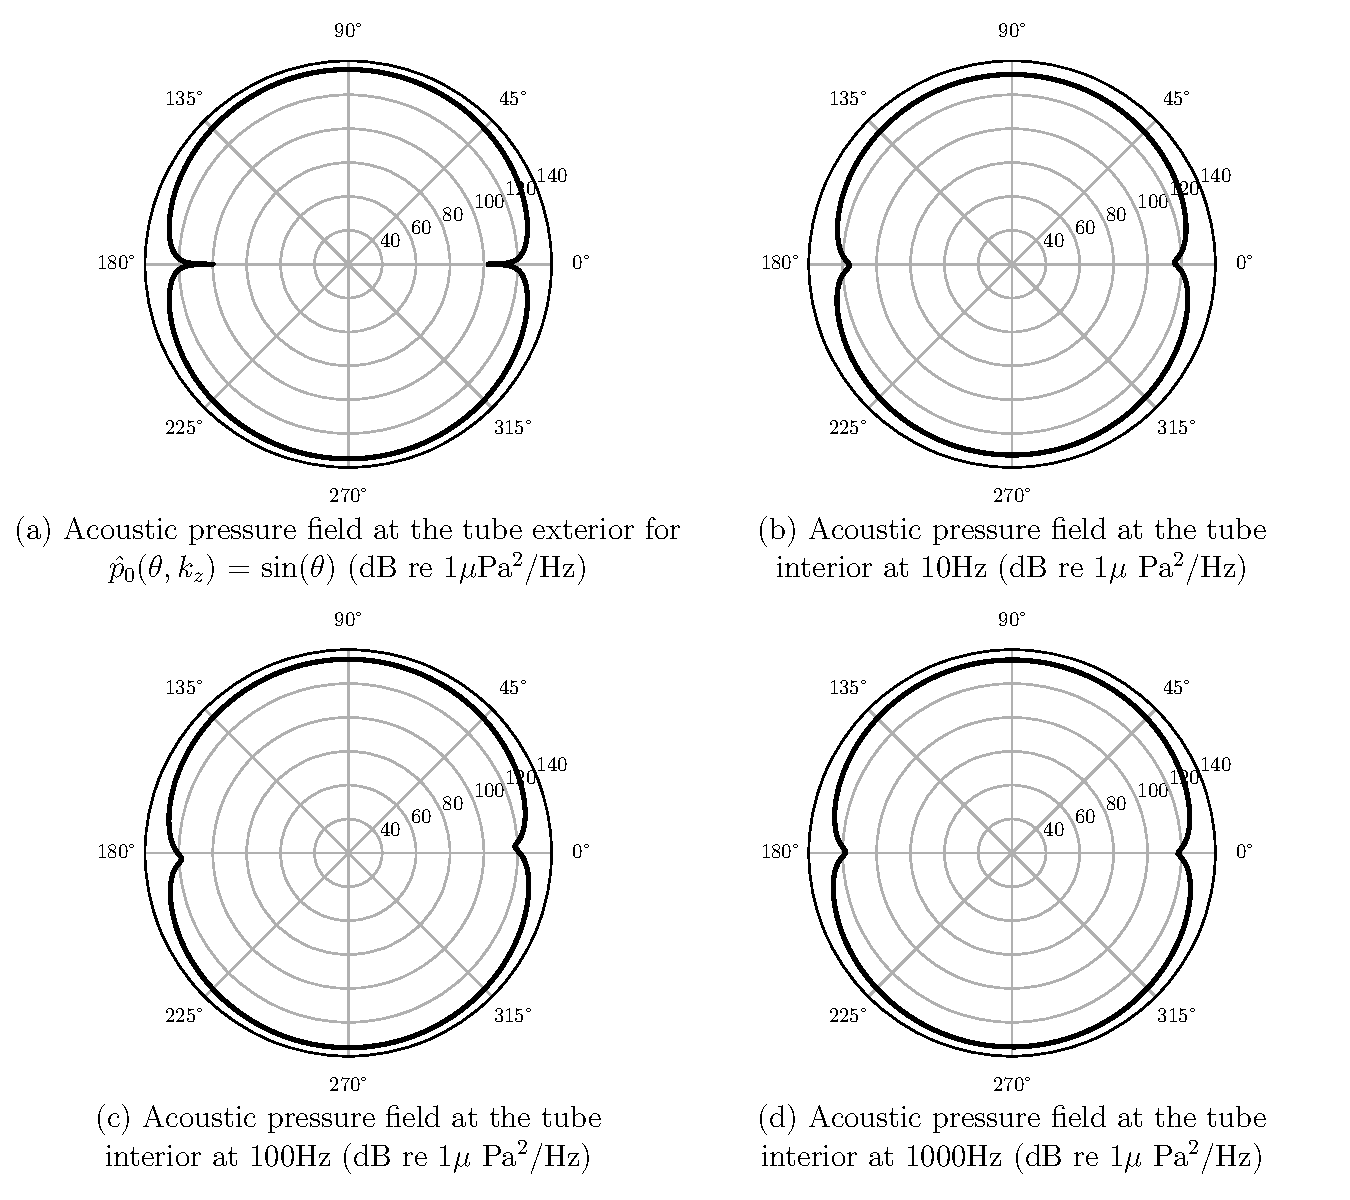
\includegraphics[width=3.1in]{figure/polarplot_sin(theta).pdf}
    \caption{(a)~External acoustic pressure field $\Hat{p}_0(\theta,k_z) =\sin(\theta)$, (b)-(d)~Acoustic pressure field at the inner surface of the tube ($r=a$) for different frequencies.}
    \label{polar plot sin theta}
\end{figure}

Figs.~\ref{polar plot sin theta}(a) and \ref{polar plot cos theta}(a) shows the resulting acoustic pressure variation (see Eqs.~(\ref{acoustic pressure field inside}), (\ref{ifft theta inside pressure}) and (\ref{SPL for theta variation}) with $\Hat{p}_f$ being replaced with $\Hat{p}_0$) along the outer surface. Figs.~\ref{polar plot sin theta}(b)~-~\ref{polar plot sin theta}(d) and Figs.~\ref{polar plot cos theta}(b)~-~\ref{polar plot cos theta}(d) depicts the azimuthal variation in the acoustic pressure (see Eqs.~(\ref{acoustic pressure field inside}), (\ref{ifft theta inside pressure}) and (\ref{SPL for theta variation})) along the tube inner surface at 10~Hz, 100~Hz and 1000~Hz for the two azimuthally different excitations. The Figs.~\ref{polar plot sin theta} and \ref{polar plot cos theta} confirms that the 3D-VA model accurately captures the azimuthal variation (restricted to $n=0$ and $n=1$) in the external pressure excitation.


\begin{figure}[h]
    \centering
    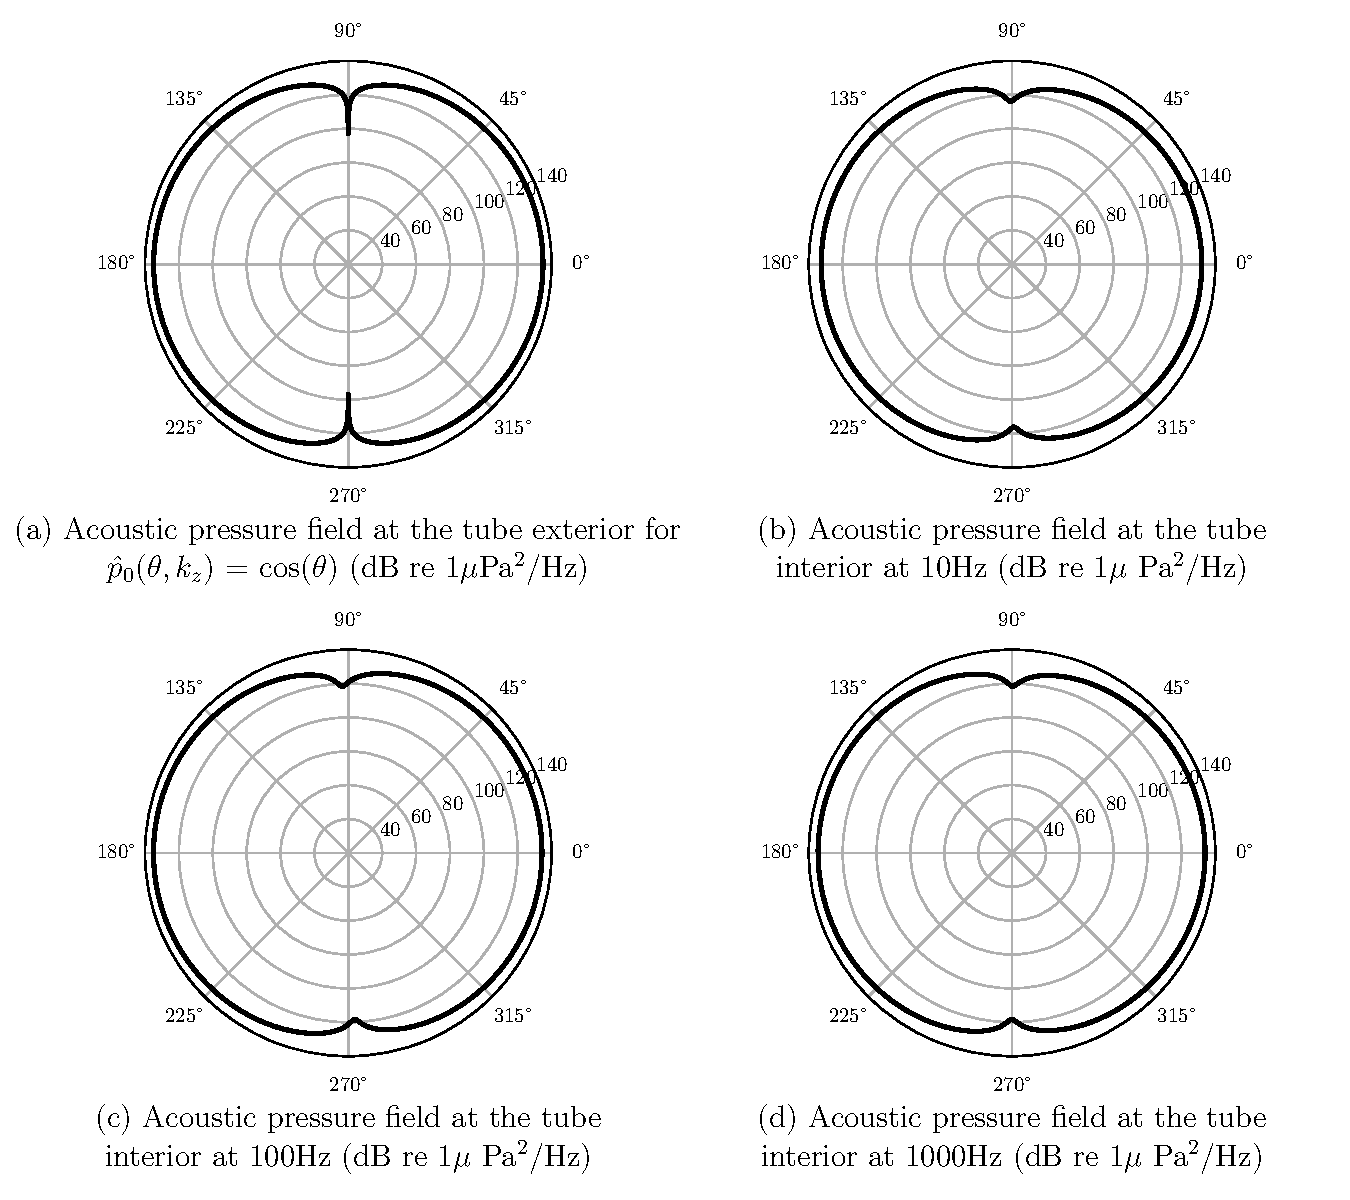
\includegraphics[width=3.1in]{figure/polarplot_cos(theta).pdf}
    \caption{(a)~External acoustic pressure field $\Hat{p}_0(\theta,k_z) =\cos(\theta)$, (b)-(d)~Acoustic pressure field at the inner surface of the tube ($r=a$) for different frequencies.}
    \label{polar plot cos theta}
\end{figure}

\begin{figure}[h]
    \centering
    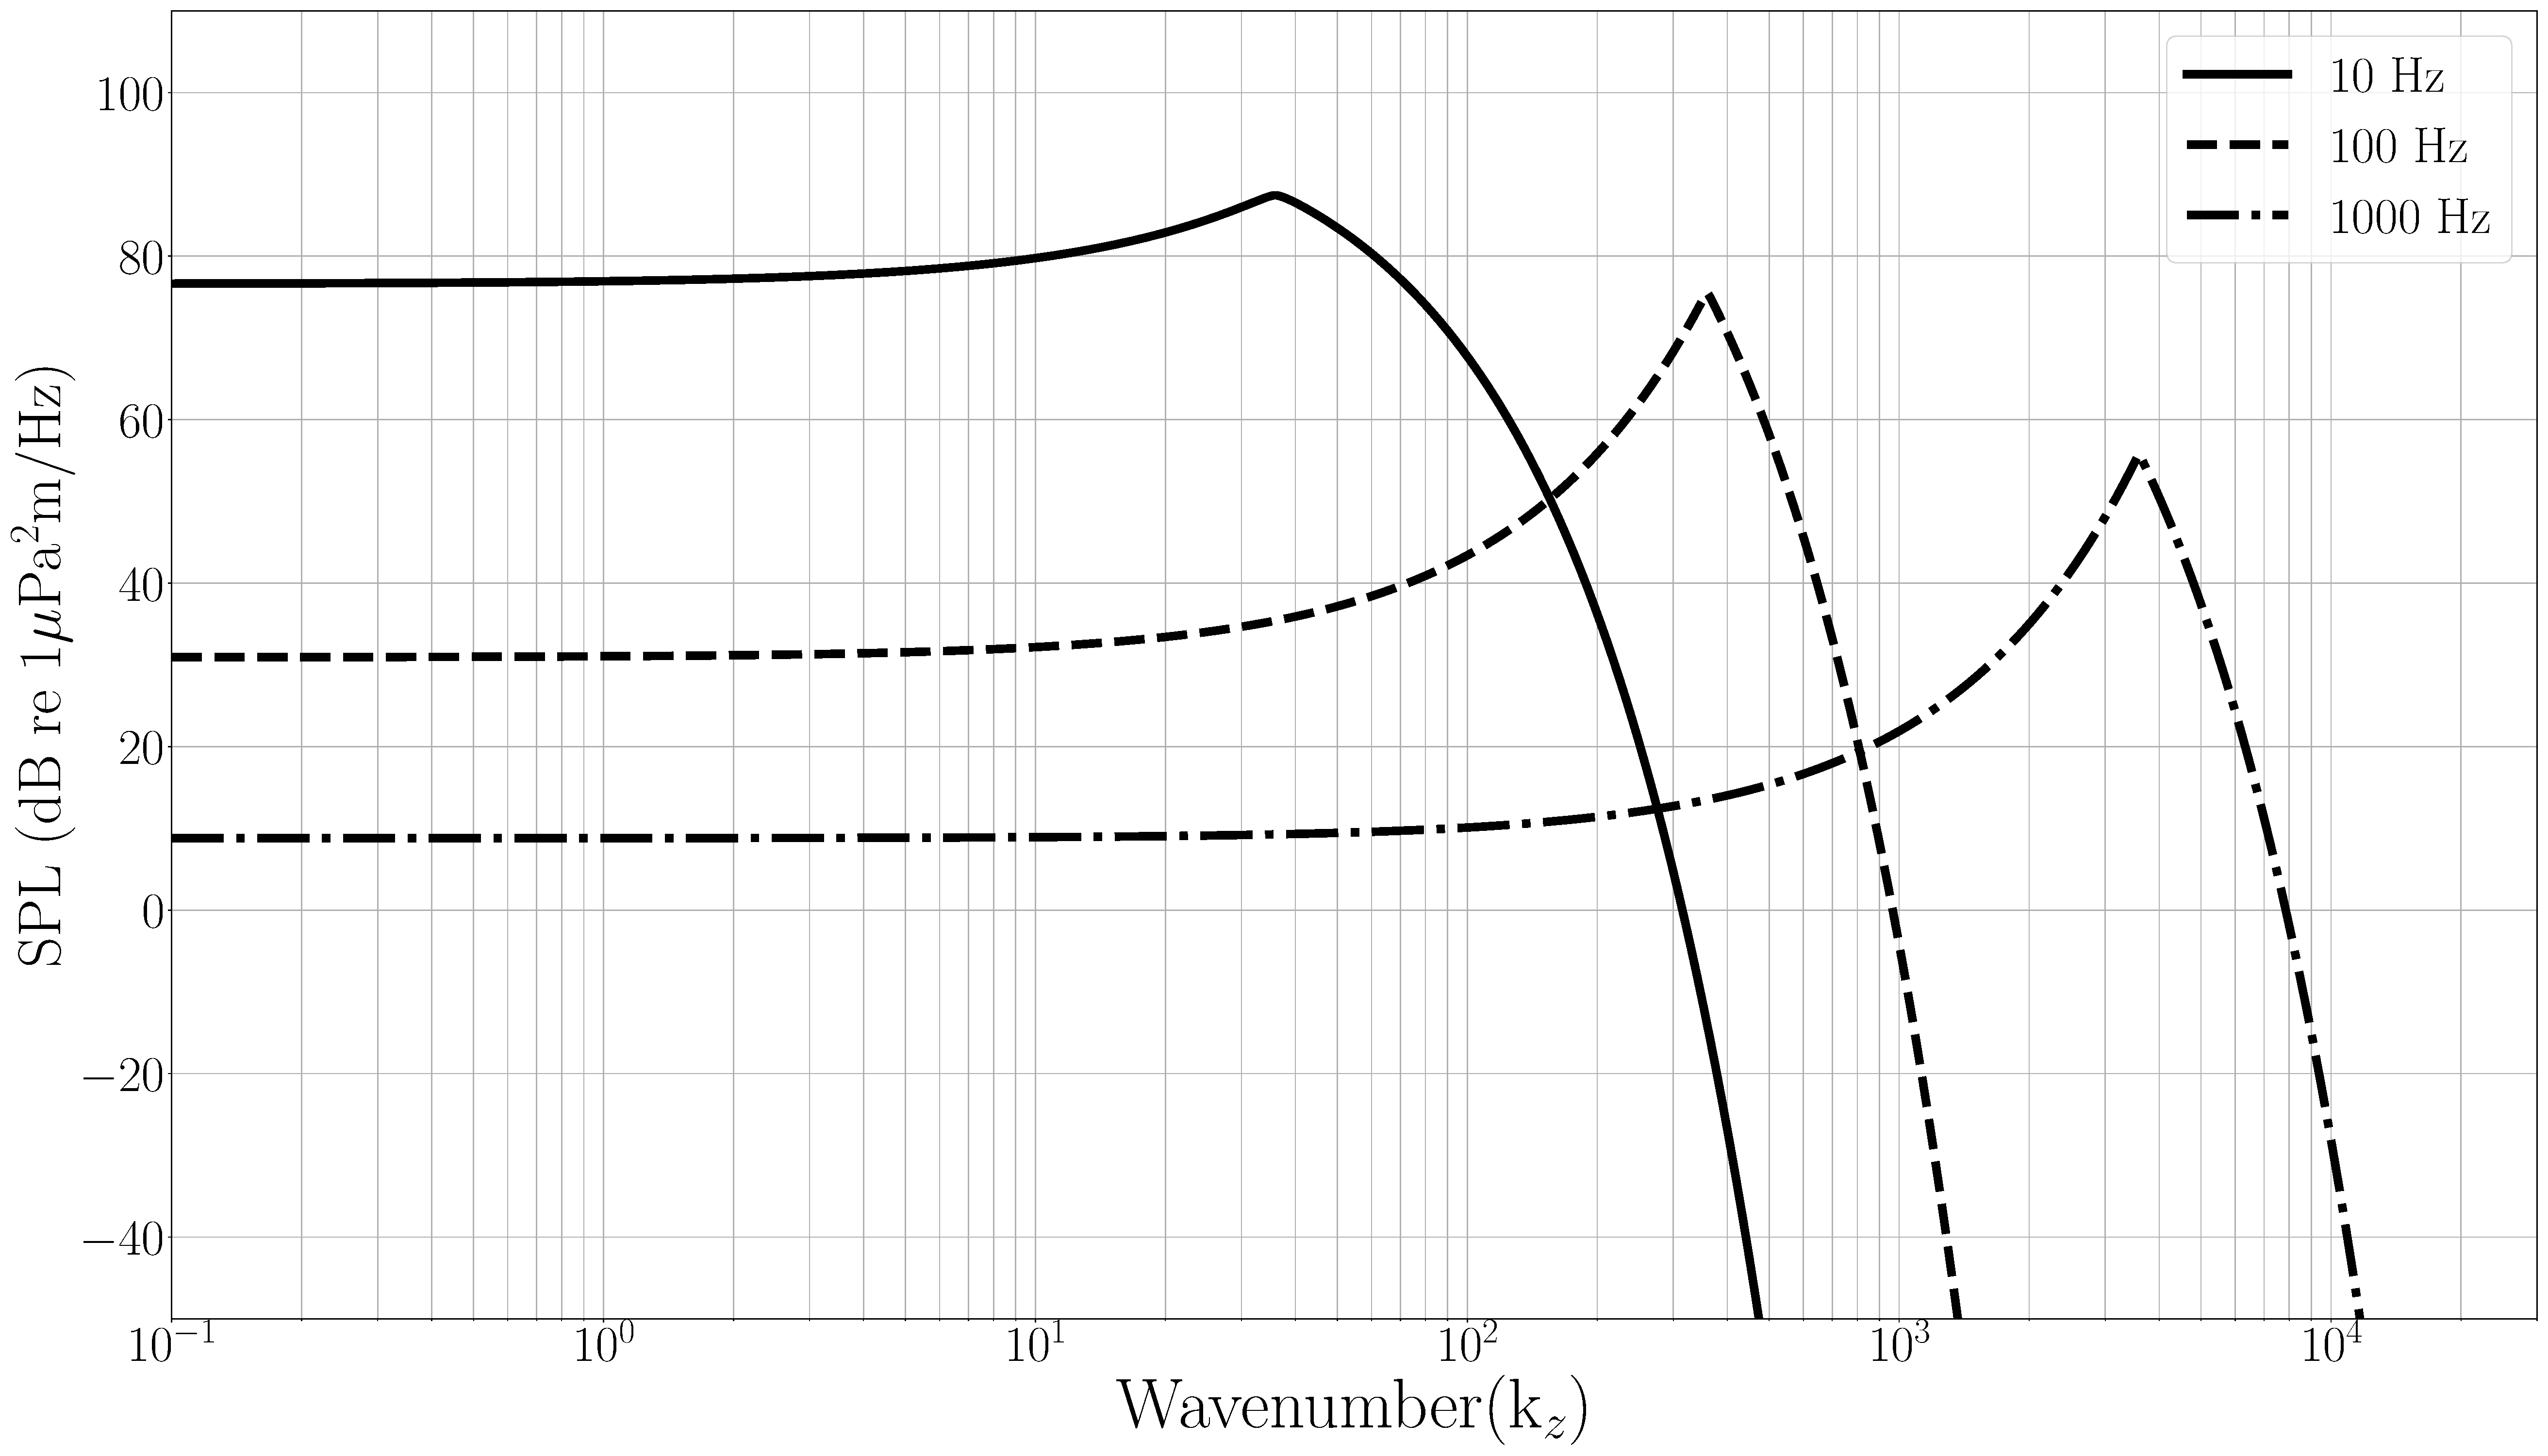
\includegraphics[width=3.1in]{figure/Comparison of turbulent pressure spectrum of Hybrid.pdf}
    \caption{The external turbulent pressure excitation at 5~knots over a tube of 40~mm diameter computed using the hybrid model~(Eq.~(\ref{hybrid model turbulent pressure})).}
    \label{Hybrid turbulent pressure spectrum}
\end{figure}


\subsection{On-axis acoustic pressure spectrum for external turbulent pressure excitation}
\label{Interior pressure}
This section presents on-axis flow noise spectrum when the elastic tube is excited by the external turbulent pressure field. The external turbulent pressure field (see Fig.~\ref{Hybrid turbulent pressure spectrum}) is computed using the present hybrid model (Eq.~(\ref{hybrid model turbulent pressure})). Further, the present 3D-VA model is used to compute the on-axis flow noise spectrum~(see Eqs.~\ref{on-axis flow noise spectrum} and \ref{SPL flow noise spectrum}). This flow noise spectrum is compared with that computed using the tube transfer function model~\cite{knight1996} (see Fig.~\ref{3d vs approx}) and the axisymmetric model~\cite{jineesh2013} (see Fig.~\ref{3d vs axi}). The elastic tube, inside fluid and hydrophone array parameters used for computation are given in Table.~\ref{tab:PresentVsJineesh}

%%%%%%%%%%%%%%%%%%%%%%%%%%%%%%%%%%%%%%%%%%%%%%%%%%%%%%%%%%%%%%%%%%%%%%
%%%%%%%%%%%%%%% begin table   %%%%%%%%%%%%%%%%%%%%%%%%%%
\begin{table}[t]
\caption{The elastic tube, interior fluid and the hydrophone array parameters used for estimation of flow noise inside the cylinder.}
\begin{center}
\label{tab:PresentVsJineesh}
\begin{tabular}{c l l}
& & \\ % put some space after the caption
 \hline
 Property & Values\\
 \hline
 Tube diameter (m)  & 0.04 \\
 \hline
 Tube thickness (m) & 0.005 \\
 \hline
 Tow speed/Flow velocity (knots) & 5 \\
 \hline
 Number of hydrophones & 50 \\
 \hline
 Length of hydrophone (m) & 0.05 \\
 \hline
 Hydrophone spacing (m) & 0.25 \\
 \hline
 Exterior fluid density (kg/m$^{3}$) & 1000 \\
 \hline
 Interior fluid density (kg/m$^{3}$) & 800 \\
 \hline
 Reference pressure ($\mu$ Pa) & 1  \\ [0.5ex]
\hline
\end{tabular}
\end{center}
\end{table}
%%%%%%%%%%%%%%%% end table %%%%%%%%%%%%%%%%%%% 
%%%%%%%%%%%%%%%%%%%%%%%%%%%%%%%%%%%%%%%%%%%%%%%%%%%%%%%%%%%%%%%%%%%%%%
It can be seen from Figs.~\ref{3d vs approx} and \ref{3d vs axi} that the on-axis acoustic pressure computed using the 3D-VA model follows the external turbulent pressure excitation given in Fig.~\ref{Hybrid turbulent pressure spectrum} - increasing upto and peaking at the convective wavenumber~($u_c = \omega/k_c$), and decreasing exponentially beyond. Thus, the flow noise inside the tube is dominated by the contribution from wavenumbers less than the convective wavenumber.

\begin{figure}[h]
    \centering
    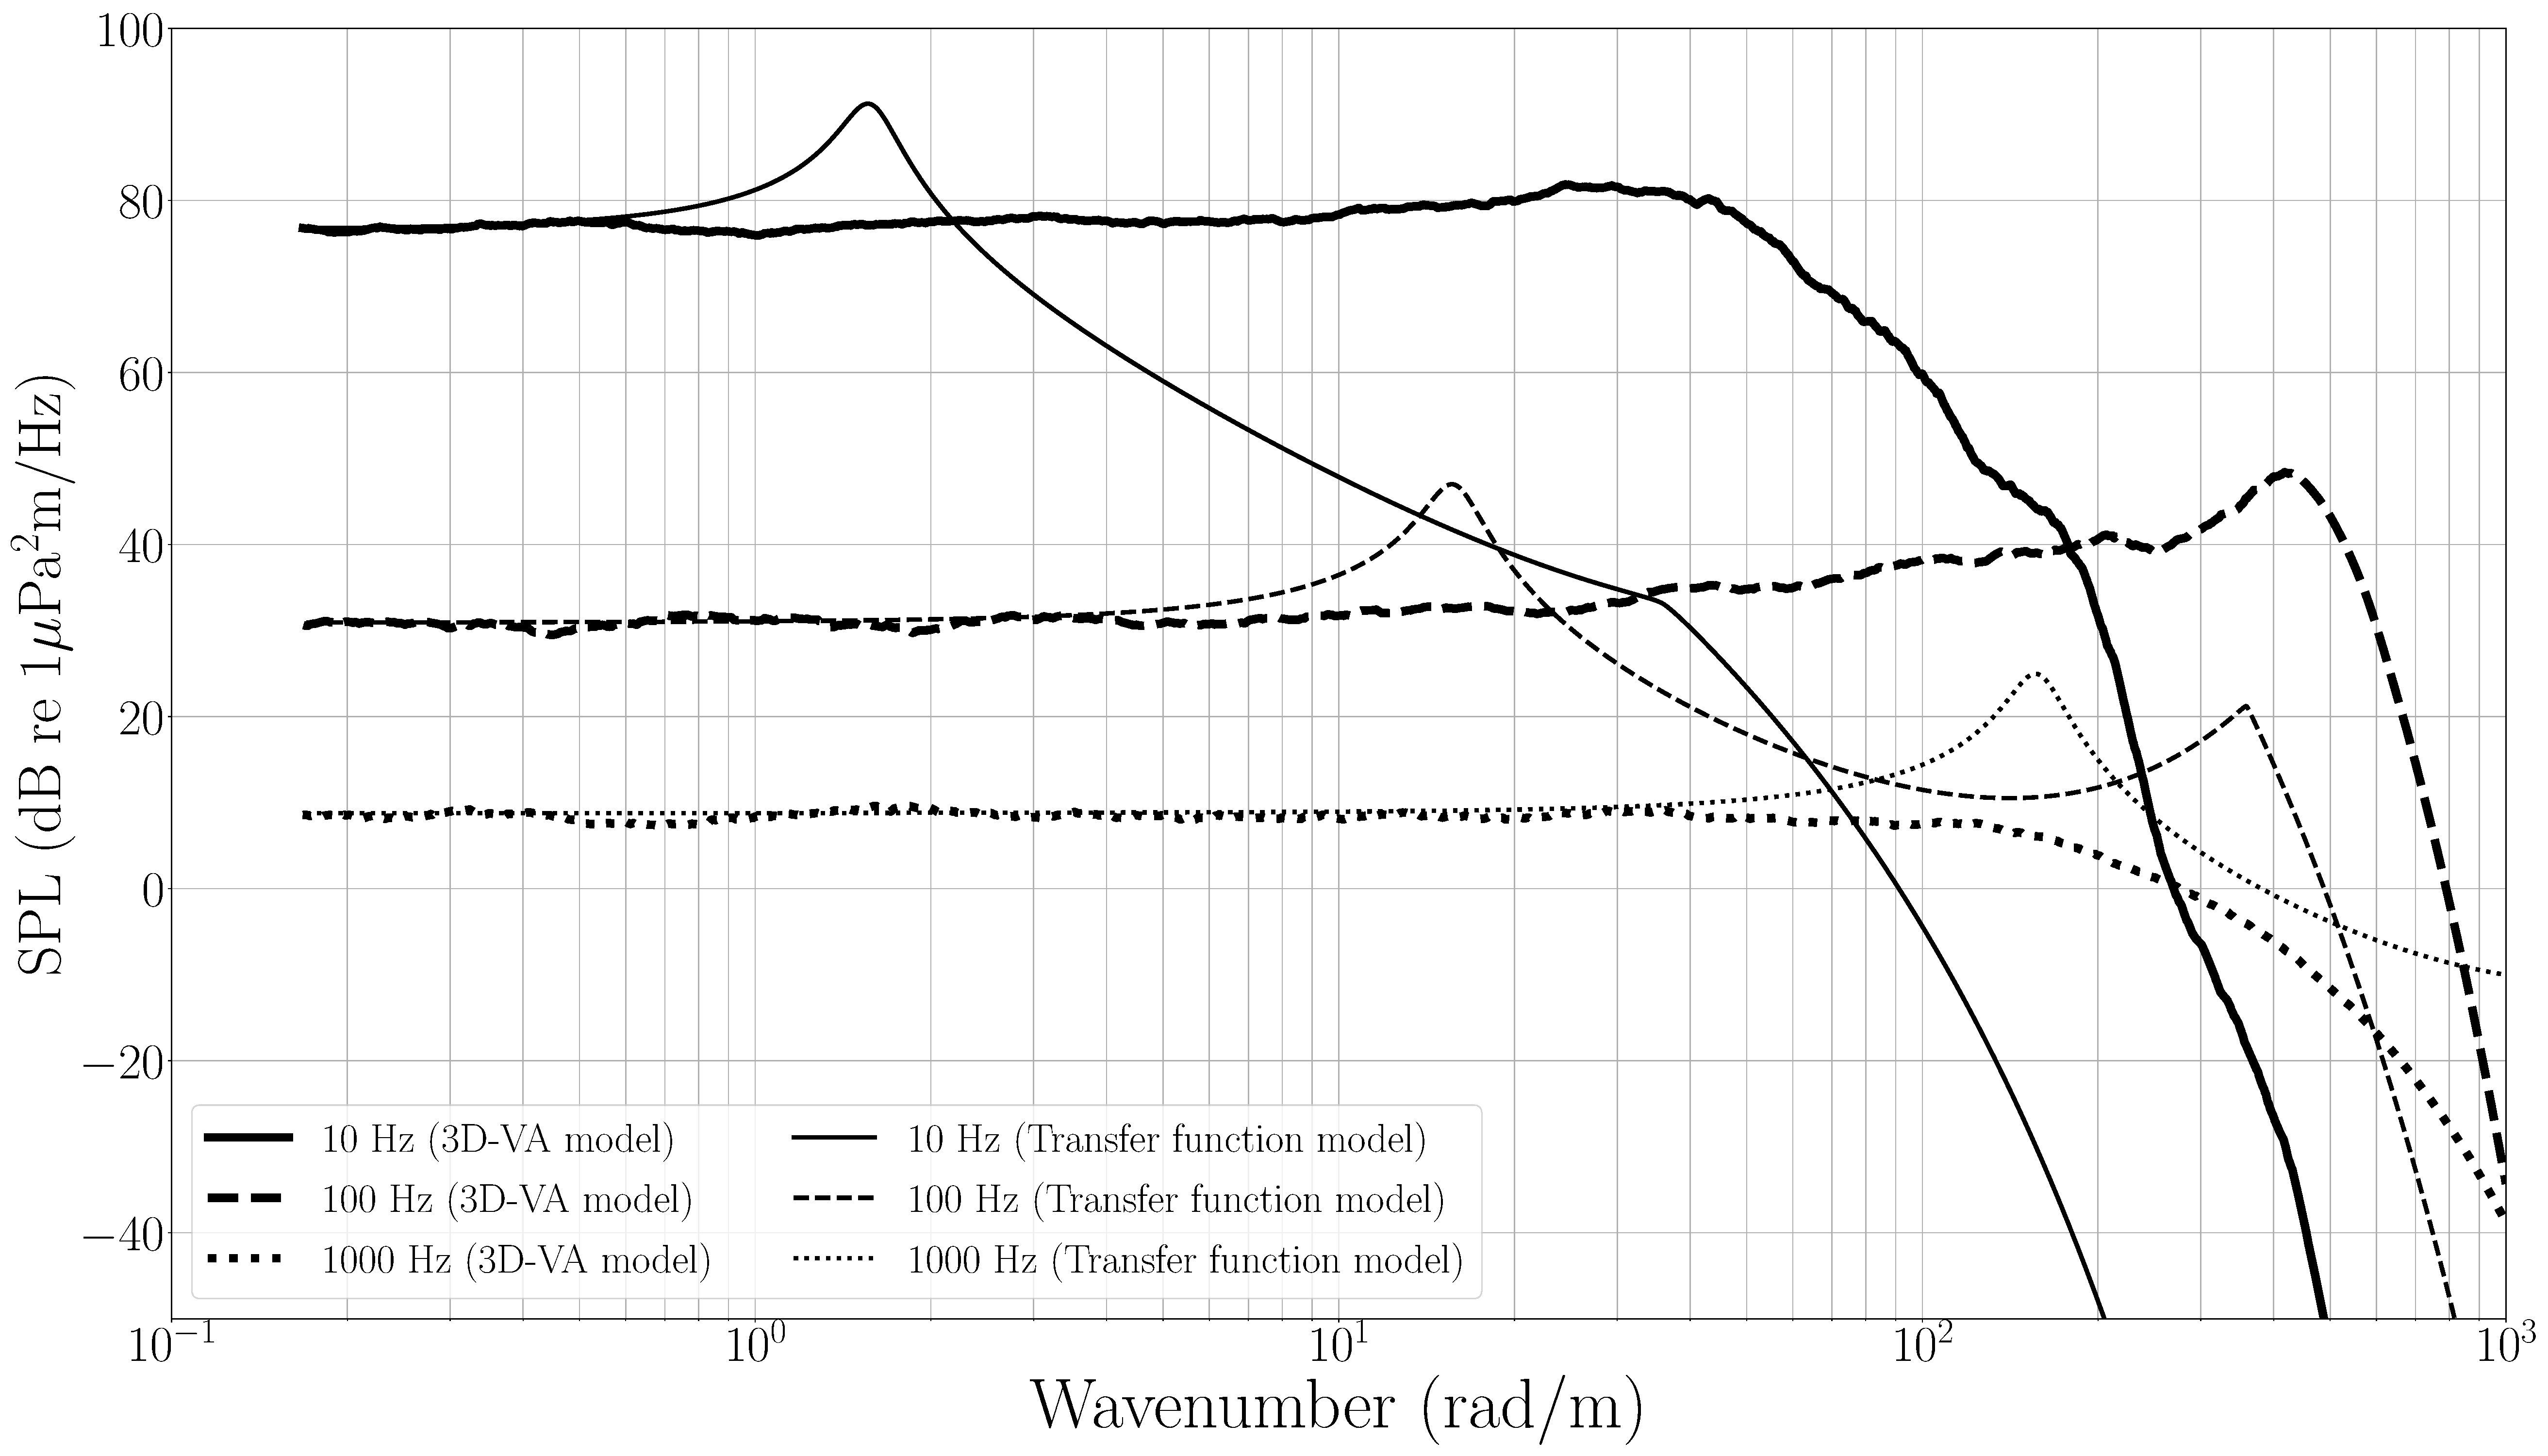
\includegraphics[width=3.1in]{figure/Inside pressure comparison 3d and approx.pdf}
    \caption{Comparison of on-axis flow noise spectrum due to a turbulent pressure excitation at 5~knots over an elastic tube of diameter 40~mm computed using the present 3D-VA model and tube transfer function model~\cite{knight1996}.} 
    \label{3d vs approx}
\end{figure}
\begin{figure}[h]
    \centering
    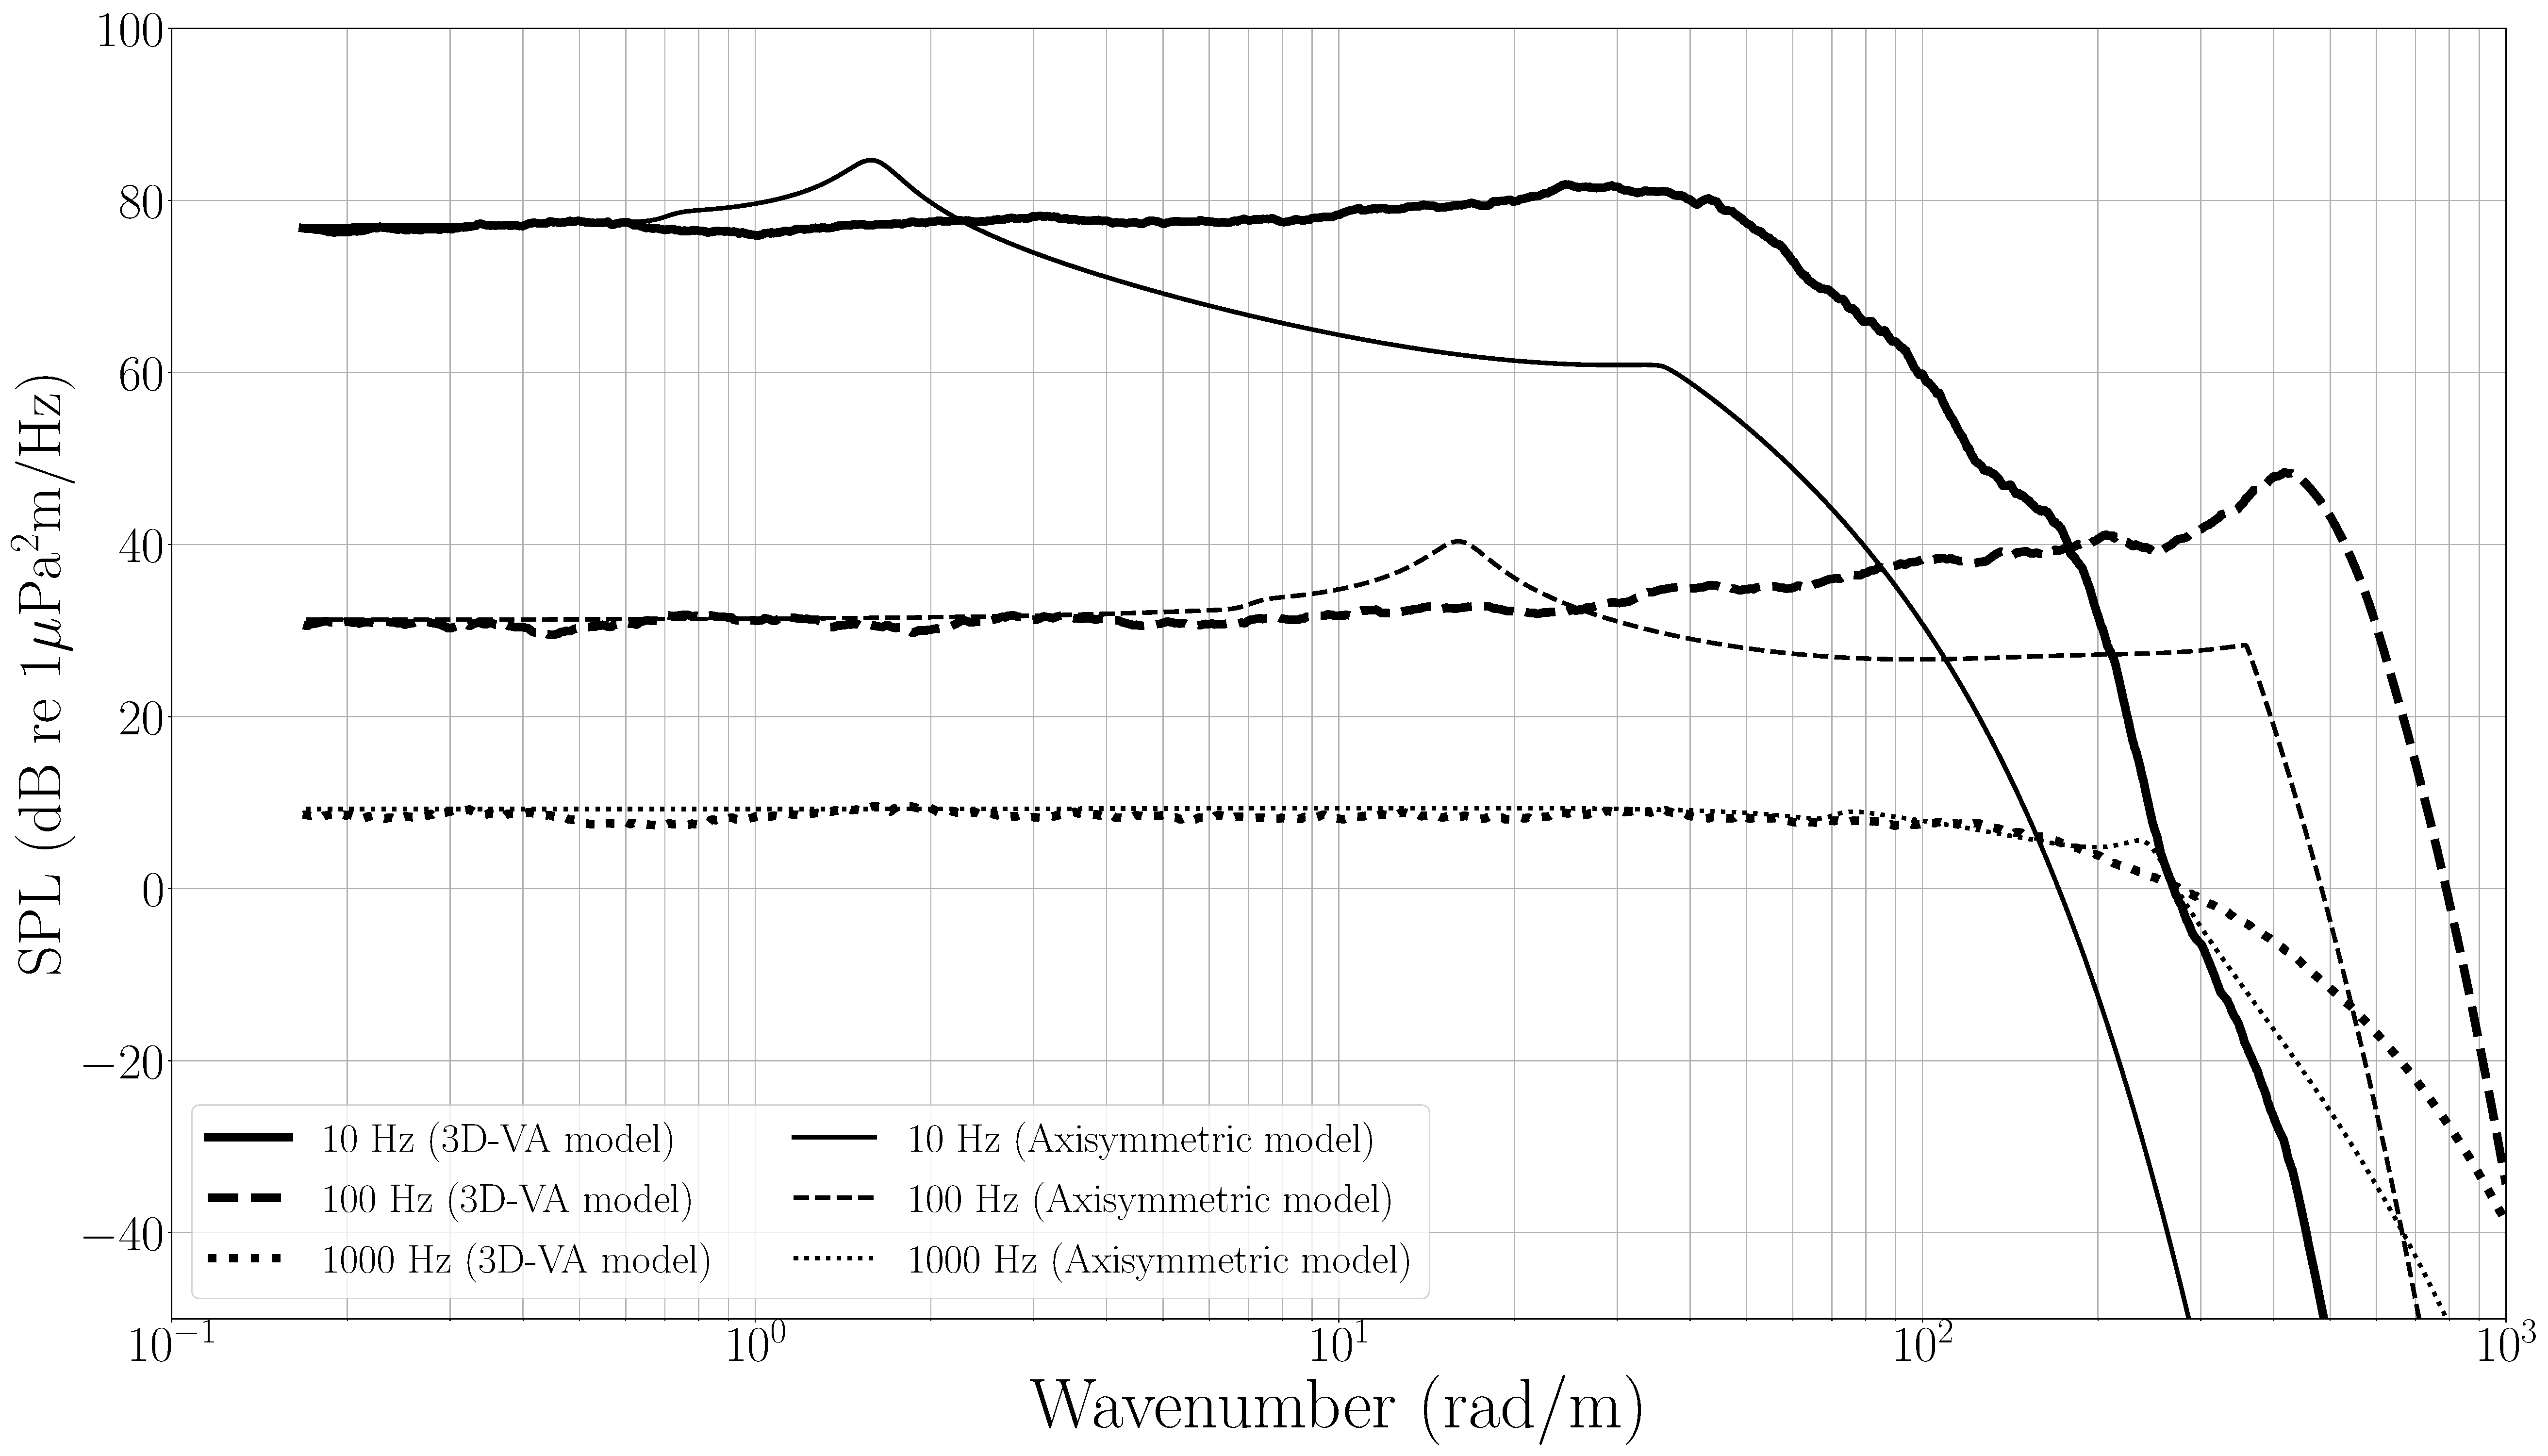
\includegraphics[width=3.1in]{figure/Inside pressure comparison 3d and axi.pdf}
    \caption{Comparison of on-axis flow noise spectrum due to a turbulent pressure excitation at 5~knots over an elastic tube of diameter 40~mm computed using the present 3D-VA model and axisymmetric model~\cite{jineesh2013}.}
    \label{3d vs axi}
\end{figure}

In the tube transfer function model (Fig.~\ref{3d vs approx}) and the axisymmetric model (Fig.~\ref{3d vs axi}) predictions, the peak occurs at a lower wavenumber than the convective wavenumber. For example, at 10~Hz, the peak occurs at $1.58$~rad/m in the tube transfer funtion model and at $1.56$~rad/m in the axisymmetric model. Note that the convective wavenumber at 10~Hz for 5~knots is $k_c = 35.93$~rad/m. This smaller wavenumber where the first peak occurs in the transfer function and the axisymmetric models corresponds to the breathing mode wavenumber, $k_b$, of the elastic tube given by~\cite{knight1996}
\begin{equation}\label{breathing wavenumber}
k_b^2 = 2\rho_0\omega^2R/Et.
\end{equation}
In Eq.~(\ref{breathing wavenumber}), $\rho_0$ is the density of the inside fluid, $R$ is the outer radius of the elastic tube, $E$ is the Young's modulus of the tube and $t$ is the thickness of the tube. The tube transfer function model and axisymmetric model consider only the breathing mode~($n=0$) variations while modelling the fluid-filled elastic tube. The present 3D-VA model considers both $n=0$~(breathing) and $n=1$~(first order) variations in the solid and fluid displacement fields. The absence of peaks at the breathing wavenumber in the present 3D-VA model indeed demonstrates a cumulative effect of including both $n=0$ and $n=1$ order terms in the fully-coupled vibroacoustic formulation. The same is the reason for the difference in flow noise spectrum between the 3D-VA model and the other models beyond the breathing wavenumber.


\subsection{On-axis flow noise for external turbulent pressure excitation}
\label{on-axis flow noise}

This section presents the flow noise as heard by the hydrophones placed inside the fluid-filled elastic tube. The flow noise is computed using Eqs.~(\ref{on axis flow noise equation}) and (\ref{spl on-axis flow noise}). Note that the flow noise at a given frequency can be obtained by integrating the corresponding flow noise spectrum~(Figs.~\ref{3d vs approx} and \ref{3d vs axi}) over the wavenumber. Fig.~\ref{3d vs knight vs jineesh} shows the variation in flow noise with frequency, computed using the present fully-coupled 3D-VA model. It also depicts the flow noise predicted by the transfer function and the axisymmetric models. Note that in all the cases, the external turbulent pressure excitation is given by Eq.~(\ref{hybrid model turbulent pressure})~(the hybrid model). The elastic tube, interior fluid and hydrophone parameters are given in Table.~\ref{tab:PresentVsJineesh}.



\begin{figure}[h]
    \centering
    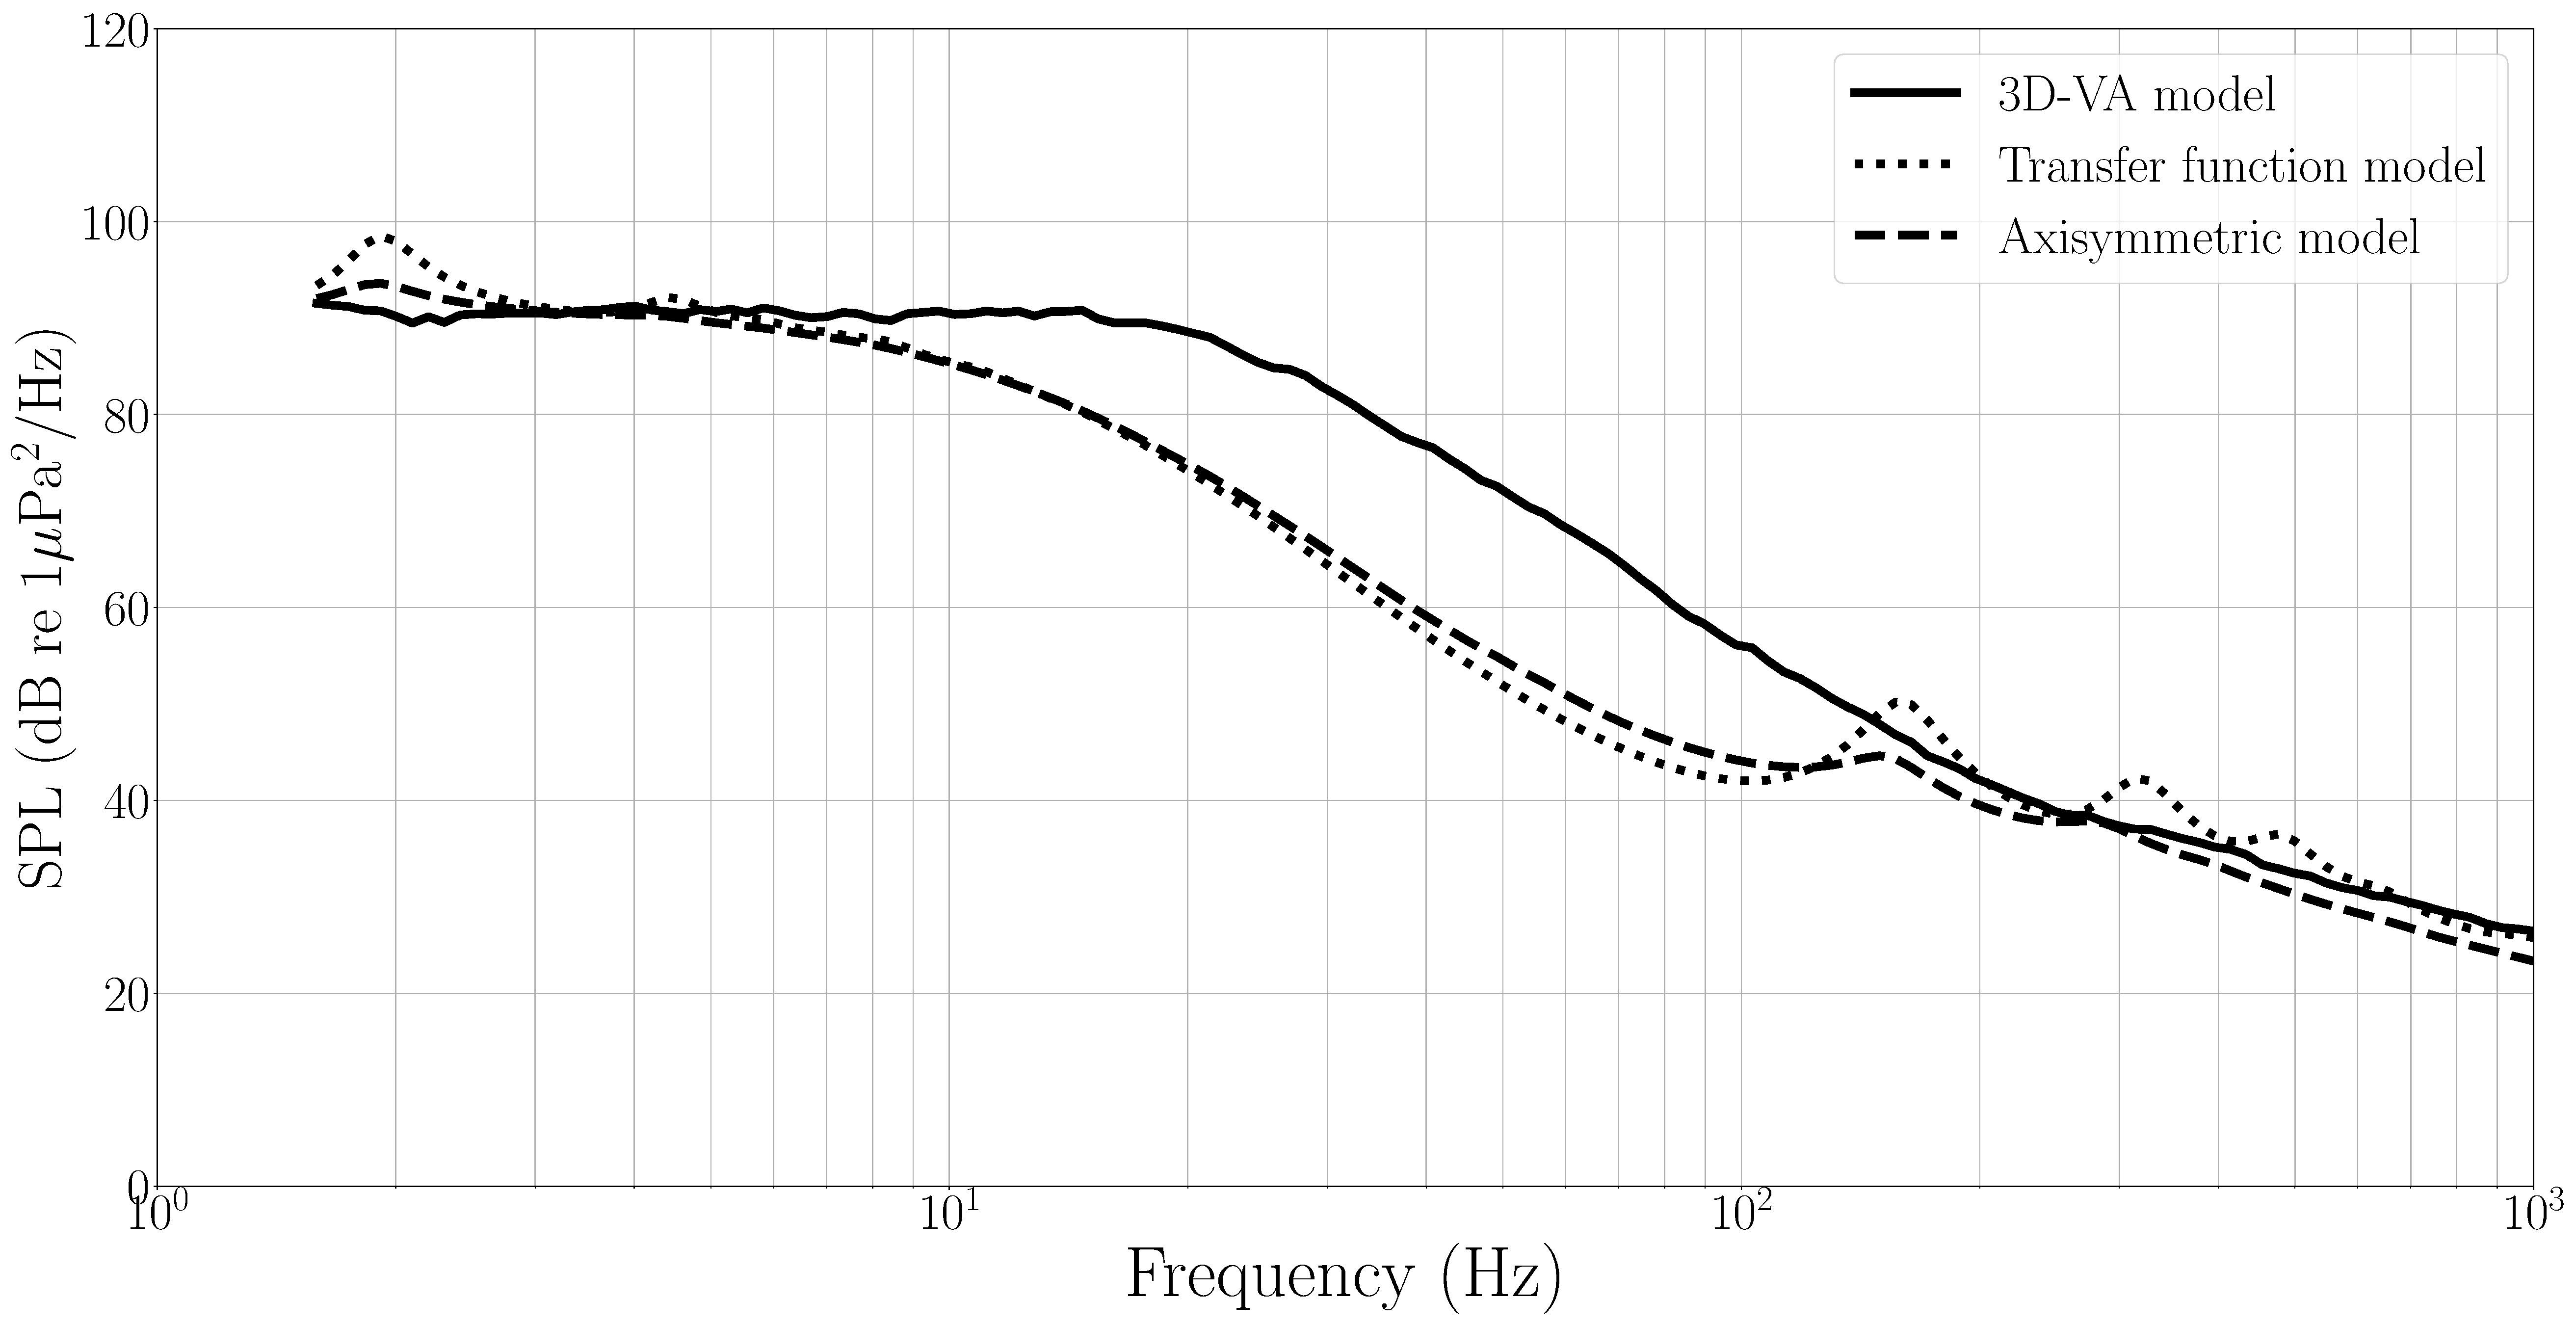
\includegraphics[width=3.1in]{figure/Flow noise comparison of 3D vs Knight and Jineesh.pdf}
    \caption{The on-axis flow noise for an elastic tube of diameter 40~mm at 5~knots due to the turbulent pressure excitation computed using the present 3D-VA model, the tube transfer function model~\cite{knight1996} and axisymmetruc model~\cite{jineesh2013}.} 
    \label{3d vs knight vs jineesh}
\end{figure}



 It can be seen from Fig.~\ref{3d vs knight vs jineesh} that the flow noise decreases with frequency. This decrease is attributed to the reduction in the external turbulent pressure excitation with frequency as shown in Fig.~\ref{Hybrid turbulent pressure spectrum}. As mentioned earlier, the 3D-VA model considers both $n=0$~(breathing) and $n=1$ variation in the acoustic pressure field. This results in a better flow noise prediction than the transfer function and axisymmetric models, where only the $n=0$ or the breathing wavenumber is considered. Note from Fig.~\ref{3d vs knight vs jineesh} that the transfer function and the axisymmetric models underpredicts the flow noise in the mid frequency range (10~Hz - 200~Hz).


\subsection{On-axis flow noise for different tube diameters and tow speeds}
\label{parametric study}

In this section, the on-axis flow noise~(Eqs.~(\ref{on axis flow noise equation}) and (\ref{spl on-axis flow noise})) is computed for different elastic tube diameters and at different tow speeds. Fig.~\ref{flow noise diff dia 3d} shows the comparison of on-axis flow noise estimated for different elastic tube diameters at 5~knots and  Fig.~\ref{flow noise diff speed 3d} shows the variation in the flow noise for a tube of 40~mm diameter at different tow speeds. The variation in flow noise is attributed to the changes in external turbulent pressure excitation with tube diameters and tow speeds as shown in Fig.~\ref{non dimensional plot of hybrid model}~(the non-dimensional plot). It was shown in Fig.~\ref{non dimensional plot of hybrid model} that the increase in diameter or decrease in tow speed result in reduction in the non-dimensional power spectral density. This leads to a decrease in the on-axis flow noise inside the fluid-filled elastic tube with increasing tube diameter~(Fig.~\ref{flow noise diff dia 3d})/decreasing tow speeds~(Fig.~\ref{flow noise diff speed 3d}).

\begin{figure}[h]
    \centering
    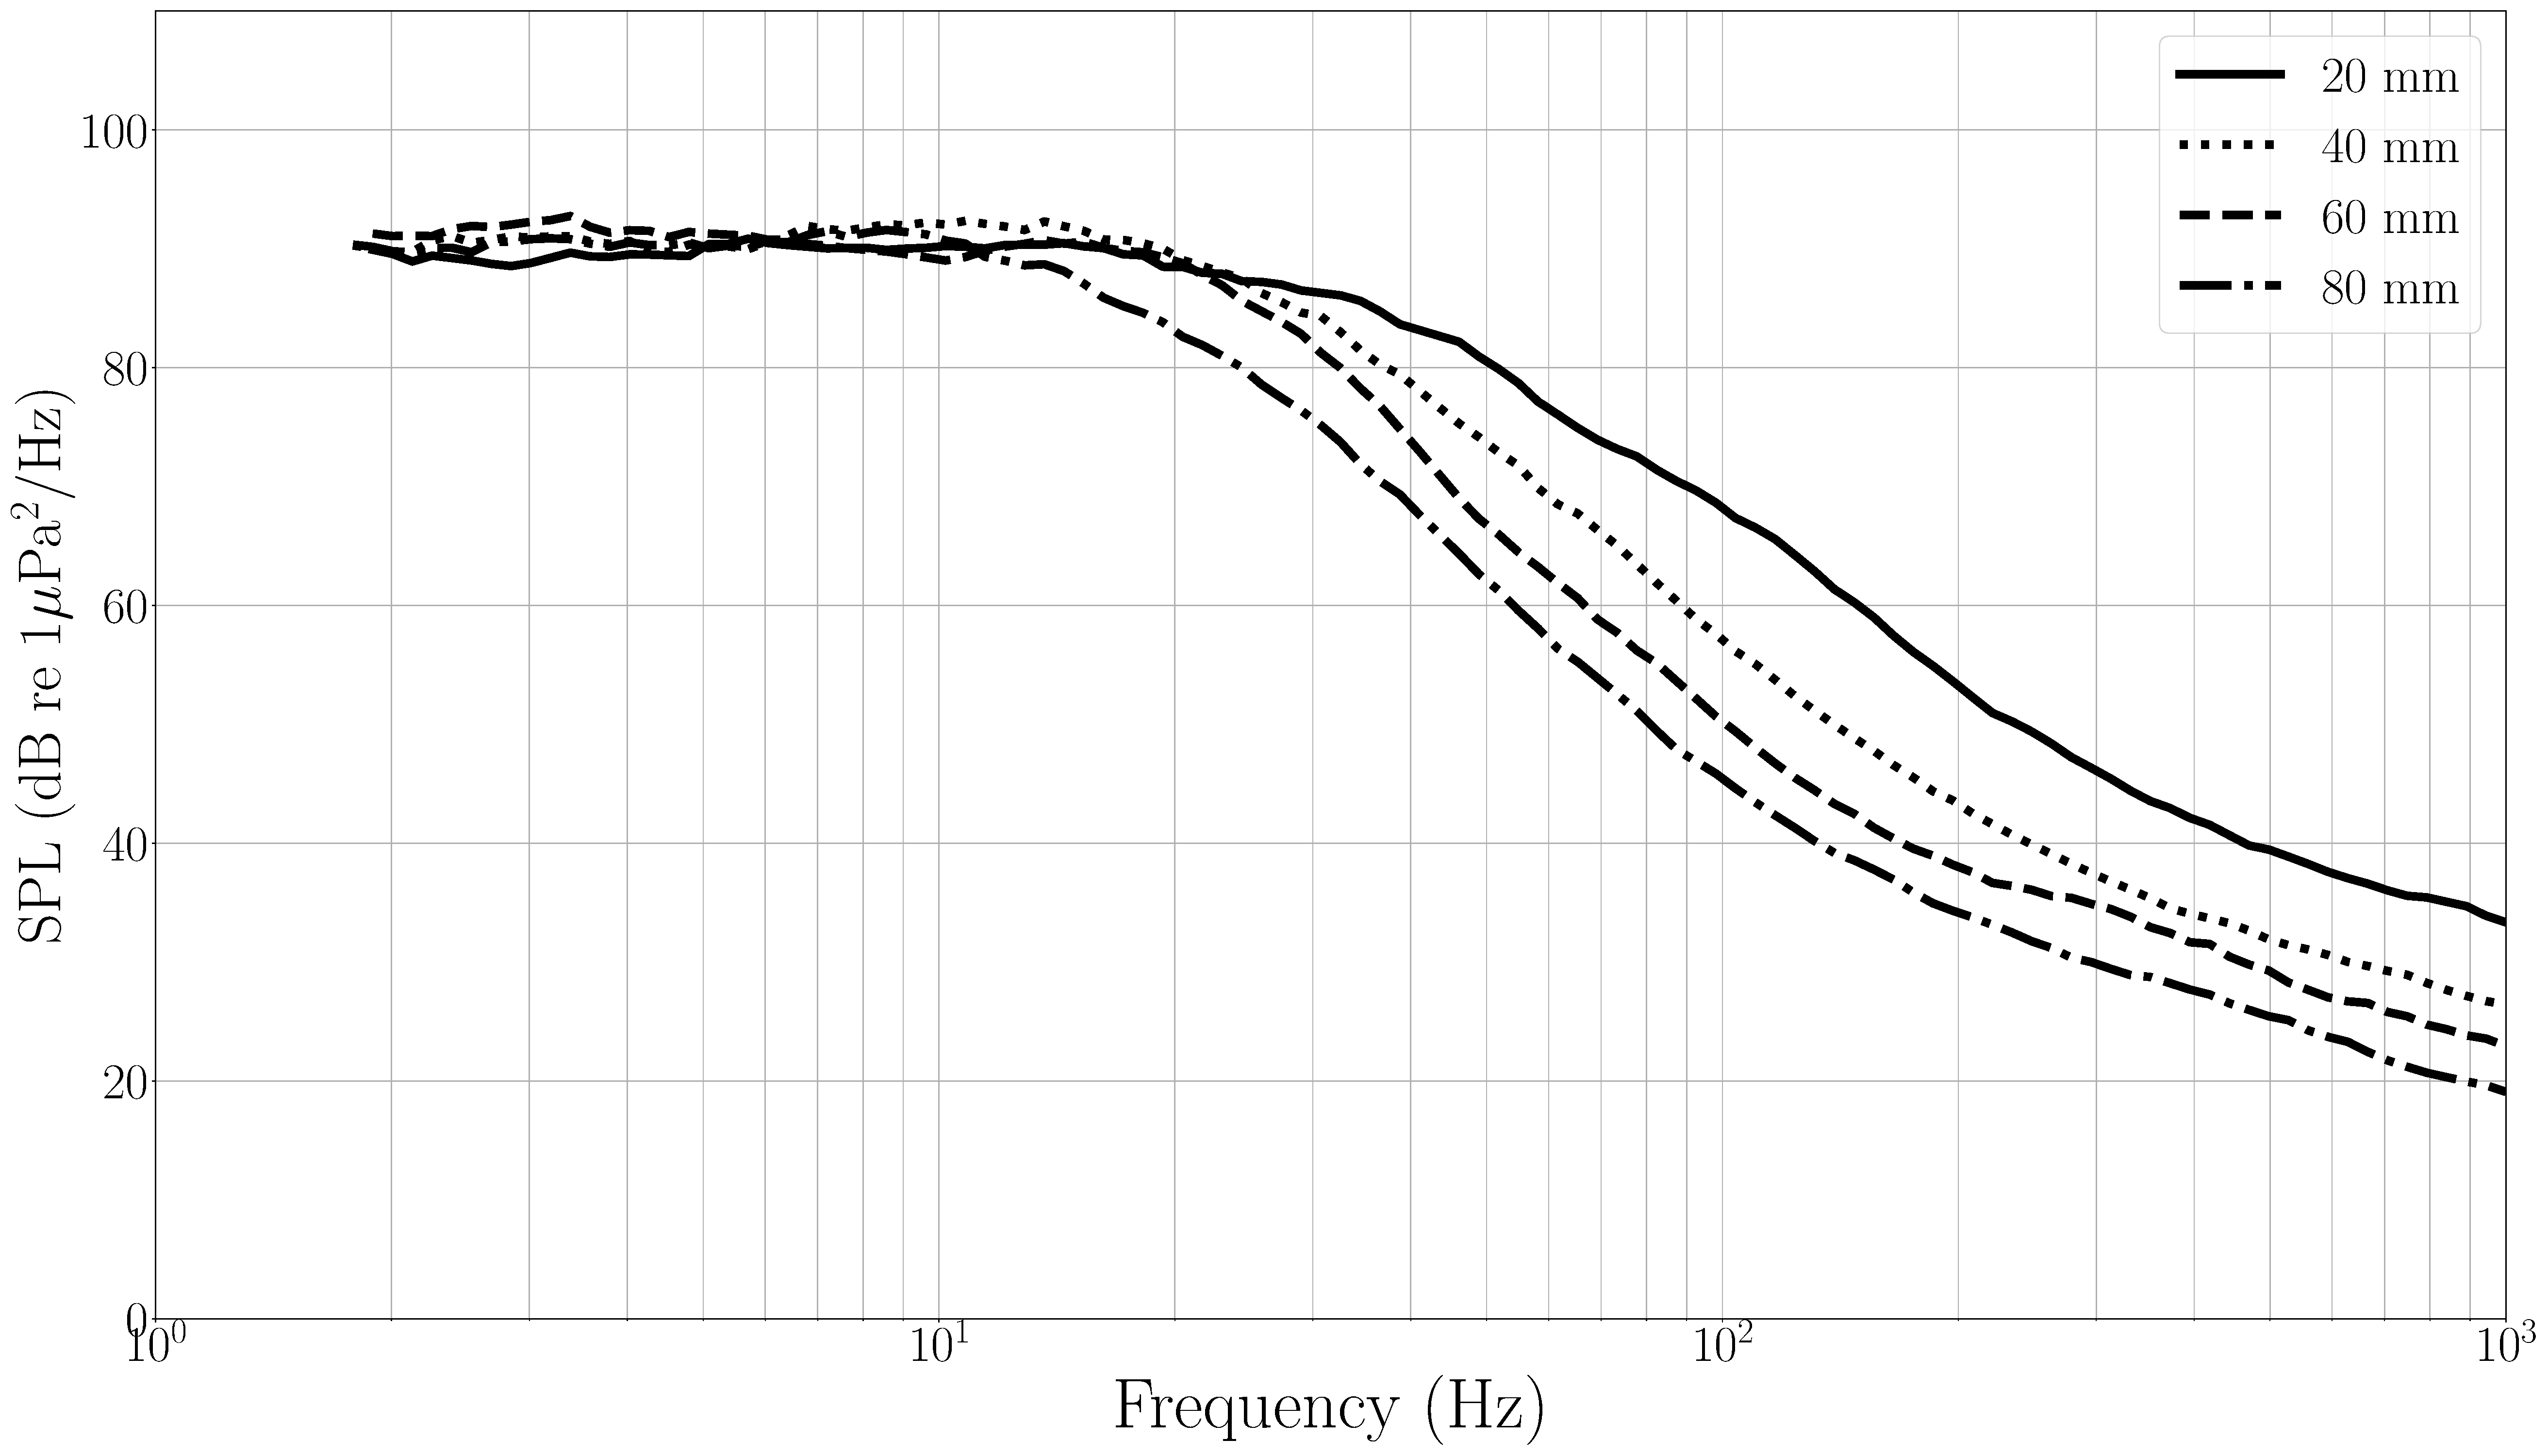
\includegraphics[width=3.1in]{figure/Comparison_of_flow_noise_3D_different_dia.pdf}
    \caption{Comparison of on-axis flow noise estimated using 3D-VA model, due to a turbulent pressure excitation at 5~knots over an elastic tube for different diameters.}
    \label{flow noise diff dia 3d}
\end{figure}

\begin{figure}[h]
    \centering
    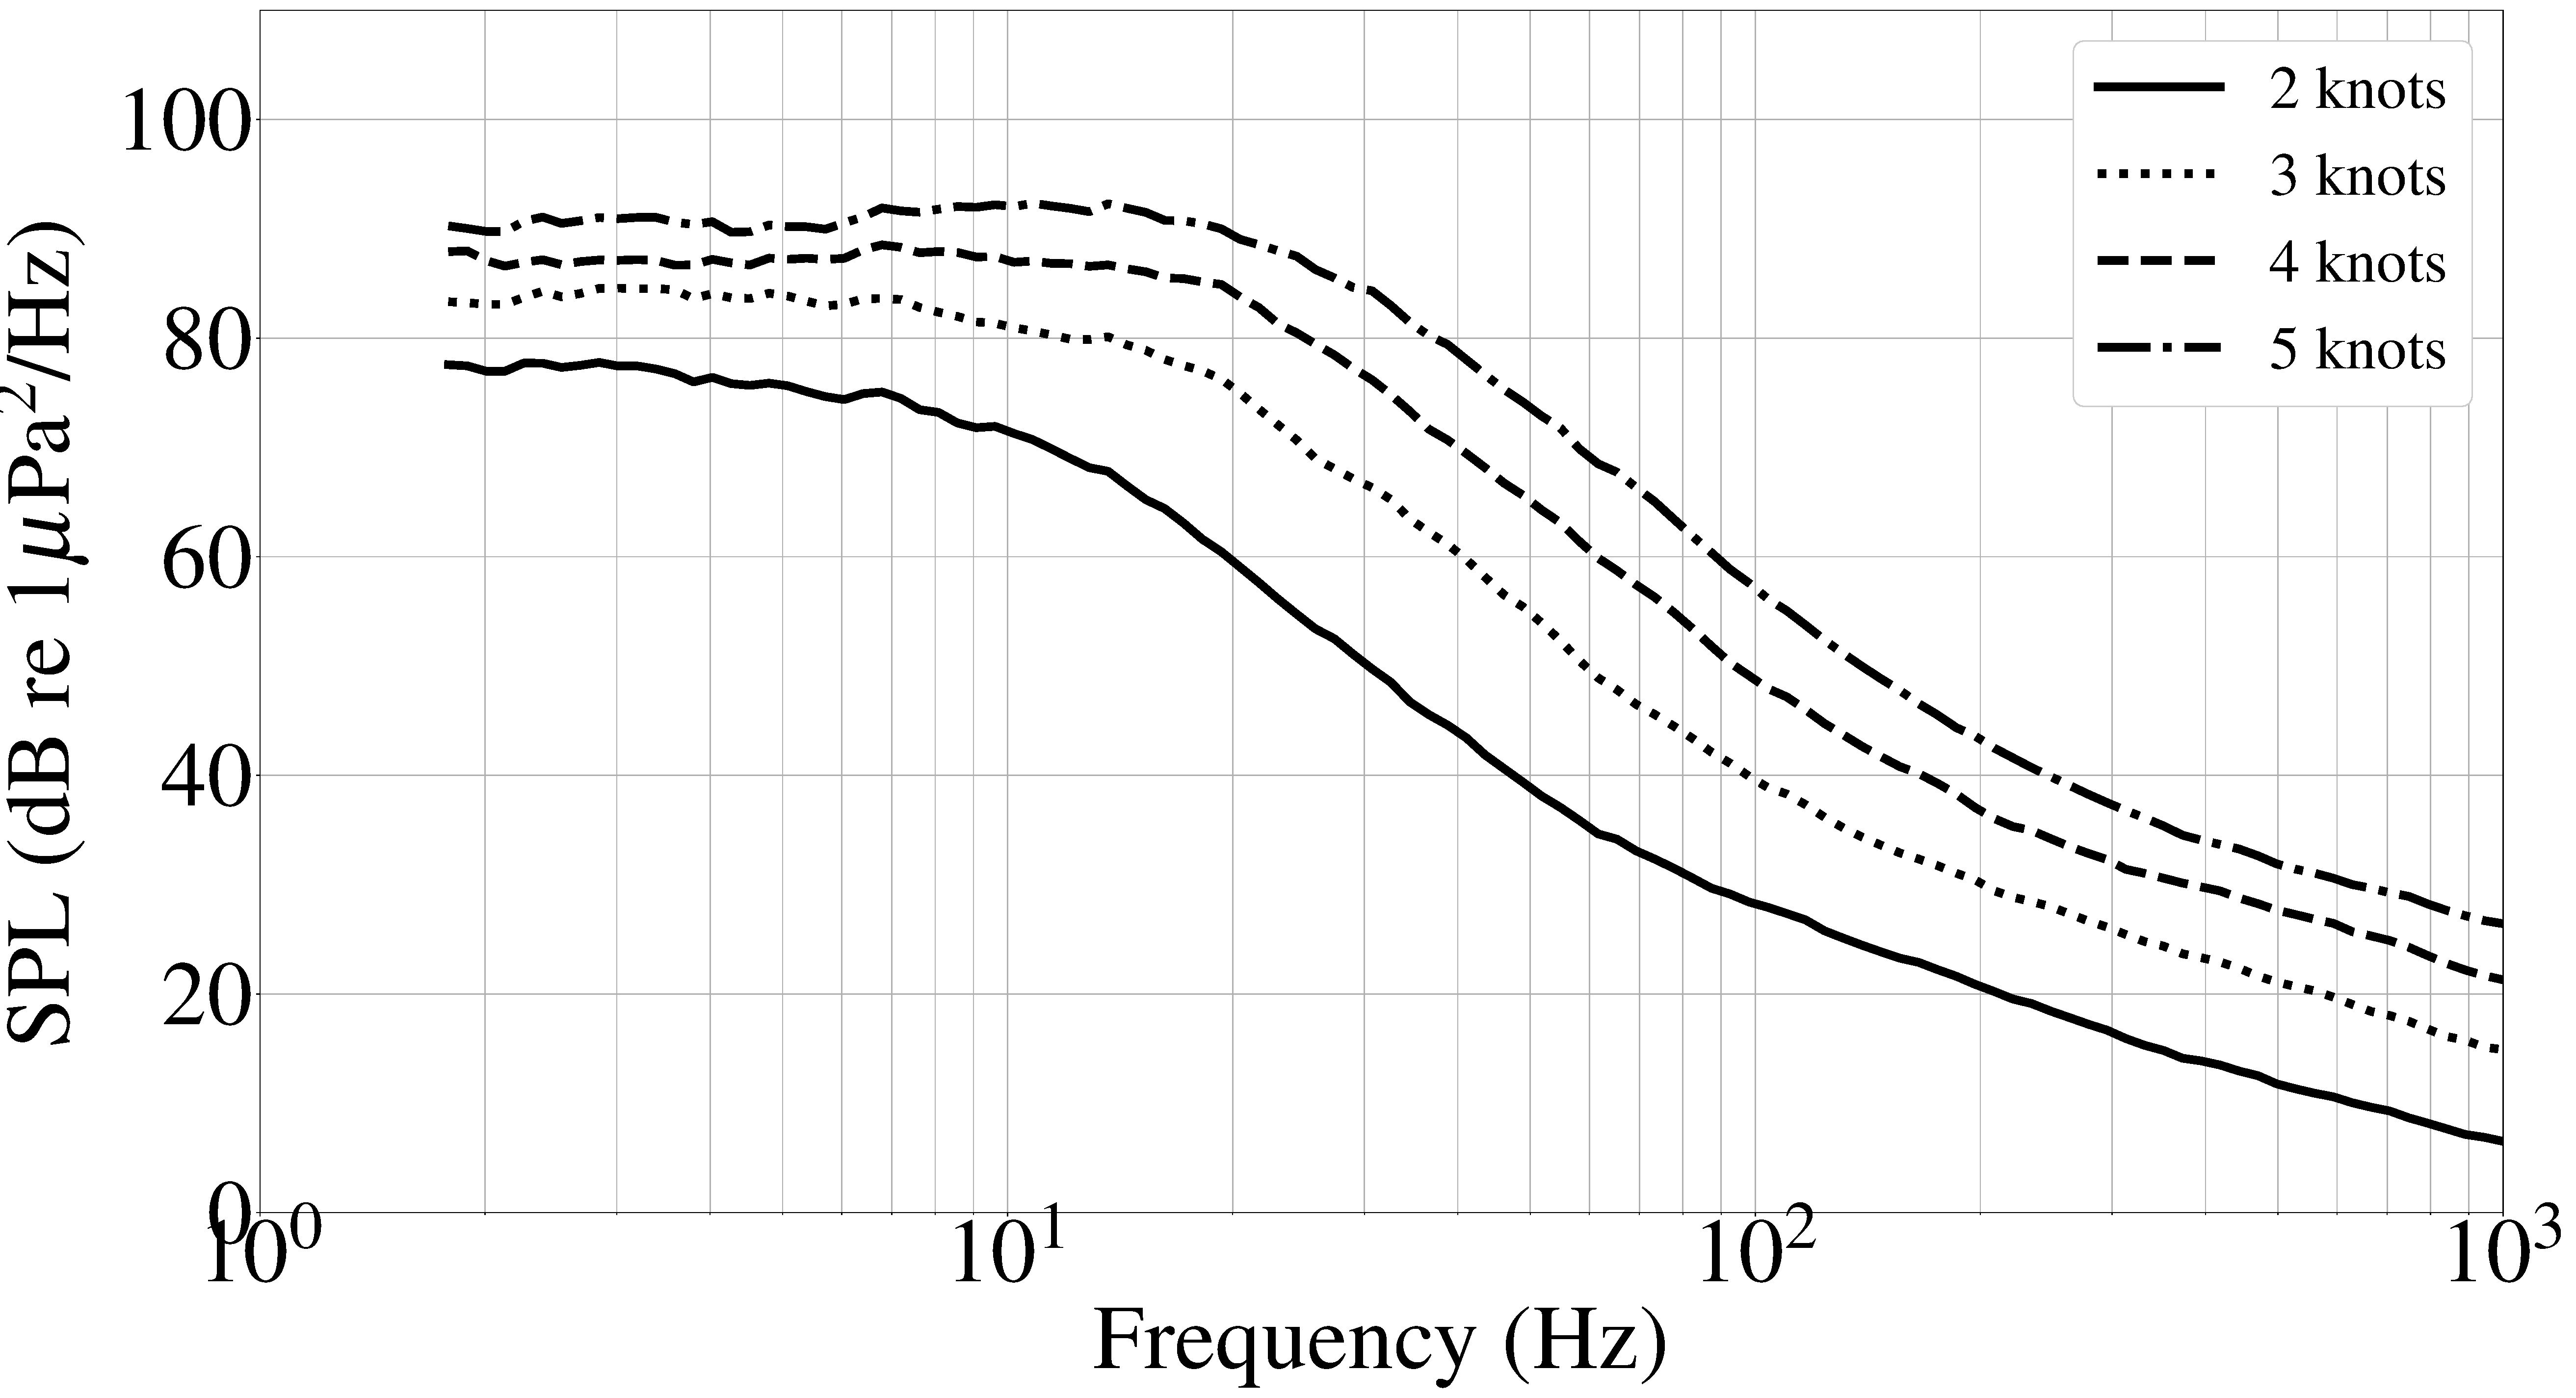
\includegraphics[width=3.1in]{figure/Comparison_of_flow_noise_3D_Different_speed.pdf}
    \caption{Comparison of on-axis flow noise estimated using 3D-VA model, due to a turbulent pressure excitation over an elastic tube of 40~mm diameter at different tow speeds.}
    \label{flow noise diff speed 3d}
\end{figure}


%%%%%%%%%%%%%%%%%%%%%%%%%%%%%%%%%%%%%%%%%%%%%%%%%%%%%%%%%%%%%%%%%%%%%%
%%%%%%%%%%%%%%%%%%%%%%%%%%%%%%%%%%%%%%%%%%%%%%%%%%%%%%%%%%%%%%%%%%%%%%
\section{Conclusions}
A new semi-empirical (hybrid) model is developed for estimating the wavenumber-frequency spectrum of turbulent pressure for an axial flow past a solid cylinder. The hybrid model is derived using insights from different turbulent pressure semi-empirical models (Chase~\cite{Chase1981} and Abdelkader Frendi et al.~\cite{frendi2020}) and the experimental results of Unnikrishnan et al.~\cite{Unni2011}. The hybrid model predictions are found to be superior to the existing semi-empirical models and compares reasonably well with available experimental results. 


A fully coupled three-dimensional vibroacoustic model~(3D-VA model) is developed for computing the pressure field inside the fluid-filled elastic tube due to external turbulent pressure excitations. In this 3D-VA model, the structure (elastic tube) is modelled using the Navier-Lame equilibrium equations and the fluid inside the tube is modelled using acoustic wave equation. The developed 3D-VA model is first tested for an exterior harmonic pressure excitation having a known azimuthal variation. It is found that the interior pressure field follows the same azimuthal variation as that of the external excitation.

Next, the 3D-VA model is used in conjunction with the hybrid model of turbulent pressure spectrum to find the on-axis flow noise. The results are then compared with the on-axis flow noise estimated using the existing transfer function model~\cite{knight1996} and the previous axisymmetric vibroacoustic model. Transfer function model and the axisymmetric model considers only the breathing mode~($n=0$) of the elastic tube but the 3D-VA model considers both $n=0$~(breathing) and $n=1$~(first order) variations in modelling the elastic tube and fluid inside the tube. Consequently, the two other models underpredict the flow noise compared to the 3D-VA model.

The on-axis flow noise is then estimated for different elastic tube diameters and at different tow speeds. At low frequencies, an increase in the tube diameter causes negligible variation in flow noise but at higher frequencies, the flow noise decreases with increase in the tube diameter. On increasing the tow speed, the flow noise is found to increase at all frequencies.


%%%%%%%%%%%%%%%%%%%%%%%%%%%%%%%%%%%%%%%%%%%%%%%%%%%%%%%%%%%%%%%%%%%%%%
\begin{acknowledgment}
This research was supported by the Defence Research and Development Organisation, India. The authors express their sincere gratitude to Dr.~Ganesh Natarajan and Dr.~Pramod Kuntikana of the Indian Institute of Technology Palakkad for their invaluable support and guidance throughout this research. Special thanks also go to Dr.~T.~Santhanakrishnan, Mr.~Sameer Abdul Azeez, Mr.~Jineesh George, Mr.~Samuel Theophilus, and Mr.~Anshath Hussain of the Naval Physical \& Oceanographic Laboratory for their invaluable feedback and assistance with this project. We extend our gratitude to Prof.~A.~Seshadri Sekhar, Director of the Indian Institute of Technology Palakkad and Dr.~Duvvuri Seshagiri, OS and Director of the Naval Physical \& Oceanographic Laboratory, for their support in enabling this collaborative research.
\end{acknowledgment}

%%%%%%%%%%%%%%%%%%%%%%%%%%%%%%%%%%%%%%%%%%%%%%%%%%%%%%%%%%%%%%%%%%%%%%
% The bibliography is stored in an external database file
% in the BibTeX format (file_name.bib).  The bibliography is
% created by the following command and it will appear in this
% position in the document. You may, of course, create your
% own bibliography by using thebibliography environment as in
%
% \begin{thebibliography}{12}
% ...
% \bibitem{itemreference} D. E. Knudsen.
% {\em 1966 World Bnus Almanac.}
% {Permafrost Press, Novosibirsk.}
% ...
% \end{thebibliography}

% Here's where you specify the bibliography style file.
% The full file name for the bibliography style file 
% used for an ASME paper is asmems4.bst.
\bibliographystyle{asmems4}

% Here's where you specify the bibliography database file.
% The full file name of the bibliography database for this
% article is asme2e.bib. The name for your database is up
% to you.
\bibliography{asme2e}

% %%%%%%%%%%%%%%%%%%%%%%%%%%%%%%%%%%%%%%%%%%%%%%%%%%%%%%%%%%%%%%%%%%%%%%
% \appendix       %%% starting appendix
% \section*{Appendix A: Stress components}\label{stress components appendix}
% In this section, the closed form of the stress equations (see section~\ref{stress components 3d}) are discussed. The normal stress equation is given by Eq.~(\ref{sigma rr 3d}). On taking fourier transform from $z-t$ domain to $k_z-\omega$ domain using Eq.~(\ref{Forward fourier transform}),
% \begin{multline}
    % \Hat{\tau}_{rr}(r,\theta,k_z,\omega) = \left(\lambda+2\mu\right)\frac{\partial \Hat{W_{e}}}{\partial r}\\ + \frac{\lambda}{r}\left(\Hat{W_{e}} + \frac{\partial \Hat{\Theta_e}}{\partial \theta} \right) - j \lambda k_z \Hat{U_e}.
% \end{multline}
    % On substituting the displacement components Eq.~(\ref{Axial displacement 3d}), Eq.~(\ref{Radial displacement 3d}) and Eq.~(\ref{Azimuthal displacement 3d}) and simplifying, the closed form of normal stress is given by
    % \begin{multline}\label{normal stress r,r 3d appendix}
        % \Hat{\tau}_{rr}(r,\theta,k_z,\omega) =\\ \Bigg\{-j\lambda k_z[J_0(r\beta_1)+J_1(r\beta_1)\cos(\theta)] +\\ \chi_1 \bigg[\frac{2\mu[J_1(r\beta_1)-J_0(r\beta_1)\cos(\theta)]}{r}\\ + \frac{4\mu J_1(r\beta_1)\cos(\theta)}{r^2 \beta_1} - (\lambda+2\mu)[J_0(r\beta_1)+\\ J_1(r\beta_1)\cos(\theta)]\beta_1 \bigg]\Bigg\}\Hat{P}_1\\ + \Bigg\{\frac{1}{r^2\beta_1}\sin(\theta)\bigg[-2r\mu \beta_1 \chi_1 J_0(r\beta_1)\\ + J_1(r\beta_1)\{4\mu \chi_1-r^2\beta_1[j\lambda k_z + (\lambda+2\mu)\beta_1 \chi_1]\}\bigg]\Bigg\}\Hat{P}_2\\ + \Bigg\{-j\lambda k_z[Y_0(r\beta_1)+Y_1(r\beta_1)\cos(\theta)]\\ + \frac{\chi_1}{r^2\beta_1}\bigg[-r\beta_1 Y_0(r\beta_1)[2\mu\cos(\theta)+r\beta_1(\lambda+2\mu)]\\ + Y_1(r\beta_1)\{4\mu\cos(\theta)\\ + r\beta_1[2\mu - r\beta_1(\lambda+2\mu)\cos(\theta)]\}\bigg]\Bigg\}\Hat{Q}_1\\ + \Bigg\{\frac{1}{r^2\beta_1}\sin(\theta)\bigg[-2r\mu \beta_1 \chi_1 Y_0(r\beta_1)\\ + Y_1(r\beta_1)\{4\mu \chi_1-r^2\beta_1[j\lambda k_z + (\lambda+2\mu)\beta_1 \chi_1]\}\bigg]\Bigg\}\Hat{Q}_2\\ + \Bigg\{-j\lambda k_z[J_0(r\beta_2)+J_1(r\beta_2)\cos(\theta)]\\ + \chi_2 \bigg[\frac{2\mu[J_1(r\beta_2)-2J_0(r\beta_2)\cos(\theta)]}{r}\\ + \frac{8\mu J_1(r\beta_2)\cos(\theta)}{r^2 \beta_2} - (\lambda+2\mu)\\ [J_0(r\beta_2)+J_1(r\beta_2)\cos(\theta)]\beta_2 \bigg]\Bigg\}\Hat{R}_1\\ +  \Bigg\{-j\lambda k_z[Y_0(r\beta_2)+Y_1(r\beta_2)\cos(\theta)]\\ + \frac{\chi_2}{r^2\beta_2}\bigg[-r\beta_2 Y_0(r\beta_2)[4\mu\cos(\theta)+r\beta_2(\lambda+2\mu)]\\ + Y_1(r\beta_2)\{8\mu\cos(\theta) + r\beta_2[2\mu - r\beta_2(\lambda+2\mu)\cos(\theta)]\}\bigg]\Bigg\}\Hat{R}_2\\ + \Bigg\{\frac{2\mu\cos(\theta)}{r^2}\bigg[-2J_1(r\beta_2) + r\beta_2J_0(r\beta_2)\bigg]\Bigg\}\Hat{S}_1\\ + \Bigg\{\frac{2\mu\cos(\theta)}{r^2}\bigg[-2Y_1(r\beta_2) + r\beta_2Y_0(r\beta_2)\bigg]\Bigg\}\Hat{S}_2\\ + \Bigg\{\frac{2\mu\sin(\theta)}{r^2}\bigg[-2J_1(r\beta_2) + r\beta_2J_0(r\beta_2)\bigg]\Bigg\}\Hat{T}_1\\ + \Bigg\{\frac{2\mu\sin(\theta)}{r^2}\bigg[-2Y_1(r\beta_2) + r\beta_2Y_0(r\beta_2)\bigg]\Bigg\}\Hat{T}_2.
    % \end{multline}
% The shear stresses are given by Eq.~(\ref{tau rz 3d}), Eq.~(\ref{tau rtheta 3d}) and Eq.~(\ref{tau ztheta 3d}). These shear stresses are transformed to wavenumber-frequency domain and can be represented as
    % \begin{equation}
        % \Hat{\tau}_{rz}(r,\theta,k_z,\omega) = \mu\left(-jk_z \Hat{W}_e + \frac{\partial \Hat{U}_e}{\partial r}\right),
    % \end{equation}
    % \begin{equation}
        % \Hat{\tau}_{r\theta}(r,\theta,k_z,\omega) = \mu\left(\frac{1}{r}\frac{\partial \Hat{W}_{e}}{\partial \theta} + \frac{\partial \Hat{\Theta}_{e}}{\partial r}-\frac{\Hat{\Theta}_e}{r}\right),
    % \end{equation}
    % and
    % \begin{equation}
        % \Hat{\tau}_{z\theta}(r,\theta,k_z,\omega) = \mu\left(-j k_z \Hat{\Theta}_{e} + \frac{1}{r}\frac{\partial \Hat{U}_{e}}{\partial \theta}\right)
    % \end{equation}
    % The displacement components are substituted in above equation and simplified as 
    % \begin{multline}\label{shear stress r,z appendix}
        % \Hat{\tau}_{rz}(r,\theta,k_z,\omega) =\\ \Bigg\{\frac{\mu}{r\beta_1}\{r\beta_1 J_0(r\beta_1)\cos(\theta) - J_1(r\beta_1)[\cos(\theta) + r\beta_1]\}\\ (\beta_1 - jk_z\chi_1)\Bigg\}\Hat{P}_1 + \Bigg\{\frac{\mu\sin(\theta)}{r\beta_1}[-J_1(r\beta_1)\\ + r\beta_1 J_0(r\beta_1)](\beta_1-jk_z\chi_1)\Bigg\}\Hat{P}_2\\ + \Bigg\{\frac{\mu}{r\beta_1}\{r\beta_1 Y_0(r\beta_1)\cos(\theta)\\ - Y_1(r\beta_1)[\cos(\theta) + r\beta_1]\}(\beta_1 - jk_z\chi_1)\Bigg\}\Hat{Q}_1\\ + \Bigg\{\frac{\mu\sin(\theta)}{r\beta_1}[-Y_1(r\beta_1) + r\beta_1 Y_0(r\beta_1)](\beta_1-jk_z\chi_1)\Bigg\}\Hat{Q}_2\\ + \Bigg\{\mu J_0(r\beta_2)\cos(\theta)(\beta_2 - jk_z\chi_2)\\ + \frac{\mu J_1(r\beta_2)}{r\beta_2}\{-\beta_2[\cos(\theta) + r\beta_2]\\ + jk_z[2\cos(\theta) + r\beta_2]\chi_2\}\Bigg\}\Hat{R}_1\\ + \Bigg\{\mu Y_0(r\beta_2)\cos(\theta)(\beta_2 - jk_z\chi_2)\\ + \frac{\mu Y_1(r\beta_2)}{r\beta_2}\{-\beta_2[\cos(\theta) + r\beta_2]\\ + jk_z[2\cos(\theta) + r\beta_2]\chi_2\}\Bigg\}\Hat{R}_2\\ + \Bigg\{\frac{-j\mu k_z}{r}J_1(r\beta_2)\cos(\theta)\Bigg\}\Hat{S}_1\\ + \Bigg\{\frac{-j\mu k_z}{r}Y_1(r\beta_2)\cos(\theta)\Bigg\}\Hat{S}_2\\ + \Bigg\{\frac{-j\mu k_z}{r}J_1(r\beta_2)\sin(\theta)\Bigg\}\Hat{T}_1\\ + \Bigg\{\frac{-j\mu k_z}{r}Y_1(r\beta_2)\sin(\theta)\Bigg\}\Hat{T}_2,
    % \end{multline}
    % \begin{multline}\label{shear stress r,theta appendix}
        % \Hat{\tau}_{r\theta}(r,\theta,k_z,\omega) =\\ \Bigg\{\frac{2}{r}\mu J_2(r\beta_1)\sin(\theta)\chi_1\Bigg\}\Hat{P}_1\\ + \Bigg\{\frac{-2}{r}\mu J_2(r\beta_1)\cos(\theta)\chi_1\Bigg\}\Hat{P}_2\\ + \Bigg\{\frac{2}{r}\mu Y_2(r\beta_1)\sin(\theta)\chi_1\Bigg\}\Hat{Q}_1\\ + \Bigg\{\frac{-2}{r}\mu Y_2(r\beta_1)\cos(\theta)\chi_1\Bigg\}\Hat{Q}_2\\ + \Bigg\{\frac{\mu\sin(\theta)\chi_2}{r^2\beta_2}[-4r\beta_2 J_0(r\beta_2) + J_1(r\beta_2)(8-r^2\beta_2^2)]\Bigg\}\Hat{R}_1\\ + \Bigg\{\frac{\mu\sin(\theta)\chi_2}{r^2\beta_2}[-4r\beta_2 Y_0(r\beta_2) + Y_1(r\beta_2)(8-r^2\beta_2^2)]\Bigg\}\Hat{R}_2\\ + \Bigg\{\frac{\mu\sin(\theta)}{r^2}[2r\beta_2 J_0(r\beta_2) + J_1(r\beta_2)(-4+r^2\beta_2^2)]\Bigg\}\Hat{S}_1\\ + \Bigg\{\frac{\mu\sin(\theta)}{r^2}[2r\beta_2 Y_0(r\beta_2) + Y_1(r\beta_2)(-4+r^2\beta_2^2)]\Bigg\}\Hat{S}_2\\ + \Bigg\{\frac{1}{r^2}\bigg[-\mu r\beta_2 J_0(r\beta_2)(2\cos(\theta) + r\beta_2)\\ + \mu J_1(r\beta_2)\{4\cos(\theta) + r\beta_2[2-r\beta_2\cos(\theta)]\}\bigg]\Bigg\}\Hat{T}_1\\ + \Bigg\{\frac{1}{r^2}\bigg[-\mu r\beta_2 Y_0(r\beta_2)(2\cos(\theta) + r\beta_2)\\ + \mu Y_1(r\beta_2)\{4\cos(\theta) + r\beta_2[2-r\beta_2\cos(\theta)]\}\bigg]\Bigg\}\Hat{T}_2
    % \end{multline}
    % and
    % \begin{multline}\label{shear stress z,theta appendix}
        % \Hat{\tau}_{z\theta}(r,\theta,k_z,\omega) =\\ \Bigg\{\frac{-\mu}{r\beta_1}J_1(r\beta_1)\sin(\theta)(\beta_1 - jk_z\chi_1)\Bigg\}\Hat{P}_1\\ +  \Bigg\{\frac{\mu}{r\beta_1}J_1(r\beta_1) \cos(\theta)(\beta_1 - jk_z\chi_1)\Bigg\}\Hat{P}_2\\ + \Bigg\{\frac{-\mu}{r\beta_1}Y_1(r\beta_1)\sin(\theta)(\beta_1 - jk_z\chi_1)\Bigg\}\Hat{Q}_1\\ + \Bigg\{\frac{\mu}{r\beta_1}Y_1(r\beta_1)\cos(\theta)(\beta_1 - jk_z\chi_1)\Bigg\}\Hat{Q}_2\\ + \Bigg\{\frac{\mu\sin(\theta)}{r}[-J_1(r\beta_2) + j r k_z \chi_2 J_2(r\beta_2)]\Bigg\}\Hat{R}_1\\ + \Bigg\{\frac{\mu\sin(\theta)}{r}[-Y_1(r\beta_2) + j r k_z \chi_2 Y_2(r\beta_2)]\Bigg\}\Hat{R}_2\\ + \Bigg\{\frac{\mu\sin(\theta)}{r}jk_z[-J_1(r\beta_2) + r\beta_2 J_0(r\beta_2)]\Bigg\}\Hat{S}_1\\ +  \Bigg\{\frac{\mu\sin(\theta)}{r}jk_z[-Y_1(r\beta_2) + r\beta_2 Y_0(r\beta_2)]\Bigg\}\Hat{S}_2\\ + \Bigg\{\frac{j\mu k_z}{r}\{-r\beta_2 J_0(r\beta_2)\cos(\theta)\\ + J_1(r\beta_2)[\cos(\theta) + r\beta_2)]\}\Bigg\}\Hat{T}_1\\ + \Bigg\{\frac{j\mu k_z}{r}\{-r\beta_2 Y_0(r\beta_2)\cos(\theta)\\ + Y_1(r\beta_2)[\cos(\theta) + r\beta_2)]\}\Bigg\}\Hat{T}_2.
    % \end{multline}
% From section~\ref{governing equation for 3d cylinder} and section~\ref{inside fluid modelling}, there are ten independent unknown variables which have to be solved to find the pressure inside the elastic tube. The closed form expressions of boundary conditions required for solving the unknown variables are discussed in \ref{boundary condition 3d appendix}. 

% %%%%%%%%%%%%%%%%%%%%%%%%%%%%%%%%%%%%%%%%%%%%%%%%%%%%%%%%%%%%%%%%%%%%%%
% \section*{Appendix B: Head of Second Appendix}
% \subsection*{Subsection head in appendix}
% The equation counter is not reset in an appendix and the numbers will
% follow one continual sequence from the beginning of the article to the very end as shown in the following example.
% \begin{equation}
% a = b + c.
% \end{equation}

\end{document}
